% Maastricht University Thesis Template
%
% Developed for my Master Thesis at Maastricht University.
% Based on Eugenio Senes's template at the University of Torino.
%
% By Joeri Hermans (joeri@joerihermans.com)
%
% Released under an MIT license. Share, modify and enjoy, but quote the author!

% Uncomment this line if we want a book with one-sided pages.
% \documentclass[10pt, a4paper, oneside]{book}
\documentclass[10pt, a4paper]{book}

% Define the packages.
% Packages are mostly based on the NIPS (Neural Information Processing Systems) requirements.
\usepackage[T1]{fontenc}              % Use 8-bit T1 fonts
\usepackage[backend=bibtex]{biblatex} % Citing
\usepackage[english]{babel}           % Set English as main language
\usepackage[intoc, english]{nomencl}  % Nomenclature
\usepackage[utf8]{inputenc}           % Allow utf-8 input
\usepackage{algorithmicx}             % Algorithms (pseudoecode)
\usepackage{amsfonts}                 % Blackboard math symbols
\usepackage{amsmath}                  % AMS Math
\usepackage{amssymb}                  % AMS Symbols
\usepackage{appendix}                 % Appendix
\usepackage{booktabs}                 % Professional-quality tables
\usepackage{caption}                  % Captions
\usepackage{csquotes}                 % Context sensitive quotation facilities
\usepackage{float}                    % Float control
\usepackage{geometry}                 % Easily define margins
\usepackage{graphicx}                 % Graphic materials (e.g., images)
\usepackage{hyperref}                 % Hyperlinks
\usepackage{microtype}                % Microtypography
\usepackage{rotating}                 % Allow page rotation (e.g., for large table)
\usepackage{tikz}                     % Drawings
\usepackage{url}                      % Simple URL typesetting

% Define page structure using Geometry.
% For printing, set right to 35mm
\geometry{a4paper, portrait, left=35mm, right=20mm, top=35mm, bottom=30mm}

% Define the core properties of your thesis.
\title{On Scalable Deep Learning and Parallelizing Gradient Descent}  % Title of the thesis
\author{Joeri R.~Hermans}                                             % Author name
\date{\today}                                                         % Publishing date
\def \university{Maastricht University}                               % University name
\def \universitycity{Maastricht}                                      % University city
\def \universitycountry{The Netherlands}                              % University country
\def \faculty{Faculty of Humanities and Sciences}                     % Faculty
\def \department{Department of Data Science \& Knowledge Engineering} % Department name

% Load the macros.
% Macro definitions for the Maastricht University Thesis Template.
%
% Developed for my Master Thesis at Maastricht University.
% Based on Eugenio Senes's template at the University of Torino.
%
% By Joeri Hermans (joeri@joerihermans.com)
%
% Released under an MIT license. Share, modify and enjoy, but quote the author!

\makeatletter

\newcommand{\makethesistitle}{
  % Draw the title.
  \begin{center}
    {\large \bf \textsc{\@title}}
  \end{center}
  % Draw the author.
  \center \small \@author
}

\newcommand{\makeinstitution}{
  \begin{center}
    \small
        {\university}\\
        {\faculty}\\
        {\department}\\
        {\universitycity, \universitycountry}
  \end{center}
}

\makeatother


% Use nice Tikz arrows.
\usetikzlibrary{arrows}
\usetikzlibrary{shapes.misc}
\usetikzlibrary{positioning}
\usetikzlibrary{decorations.pathreplacing}
\tikzset{>=latex}

% Add the bibliography database.
\addbibresource{bibliography.bib}

% Build the Nomenclature package.
\makenomenclature

\makeindex
\begin{document}

% Load the nomenclature.
% Maastricht University Thesis Template
%
% Developed for my Master Thesis at Maastricht University.
% Based on Eugenio Senes's template at the University of Torino.
%
% By Joeri Hermans (joeri@joerihermans.com)
%
% Released under an MIT license. Share, modify and enjoy, but quote the author!

% Define abbreviations.
\nomenclature{$\lambda$}{Communication period, or frequency of commits to the parameter server.}
\nomenclature{$\tilde{\theta}_t$}{Center variable, or central parametrization maintained by the parameter server.}
\nomenclature{$n$}{Number of parallel workers.}
\nomenclature{$\triangleq$}{Is defined as}
\nomenclature{$\tau$}{Staleness}
\nomenclature{$m$}{Mini-batch size}
\nomenclature{$J(\theta)$}{Loss with respect to parameterization $\theta$.}
\nomenclature{$\mathcal{L}(\theta~;~\textbf{x}~;~\textbf{y})$}{Loss function with respect to parametrization $\theta$, input $\textbf{x}$, and expected output $\textbf{y}$.}
\nomenclature{$\theta^k_t$}{Parametrization of worker $k$ at time $t$.}
\nomenclature{$\eta$}{Static learning rate}
\nomenclature{$\eta_t$}{Learning rate with respect to time $t$.}
\nomenclature{ADAG}{Asynchronous Distributed Adaptive Gradients}
\nomenclature{ASGD}{Asynchronous Stochastic Gradient Descent}
\nomenclature{CERN}{European Organization for Nuclear Research}
\nomenclature{CMS}{Compact Muon Solenoid}
\nomenclature{GD}{Gradient Descent}
\nomenclature{HEP}{High Energy Physics}
\nomenclature{EASGD}{Elastic Averaging Stochastic Gradient Descent}
\nomenclature{HL-LHC}{High Luminosity Large Hadron Collider}
\nomenclature{LHC}{Large Hadron Collider}
\nomenclature{MNIST}{Mixed National Institute of Standards and Technology database}
\nomenclature{PS}{Parameter Server}
\nomenclature{SGD}{Stochastic Gradient Descent}
\nomenclature{SE}{Statistical Efficiency}
\nomenclature{HE}{Hardware Efficiency}
\nomenclature{TE}{Temporal Efficiency}


% Start front matter.
\frontmatter
\let\cleardoublepage\clearpage
% Maastricht University Cover Page.
%
% Developed for my Master Thesis at Maastricht University.
% Based on Eugenio Senes's template at the University of Torino.
%
% By Joeri Hermans (joeri@joerihermans.com)
%
% Released under an MIT license. Share, modify and enjoy, but quote the author!

\makeatletter
\begin{titlepage}

  \vspace*{2cm}
  \center \Large Master Thesis
  \center \line(1,0){200}
  \vspace{0.1cm}
  \makethesistitle
  \vspace{0.1cm}
  \center \line(1,0){200}
  \vspace{0.3cm}
  \center \small Master Thesis \id
  \vspace{2cm}
  \begin{center}
    \small
    Thesis submitted in partial fulfillment of the requirements\\ for the degree of Master of Science of Artificial Intelligence
  \end{center}
  \vspace{.5cm}
  \begin{center}
        \small \textbf{Thesis Committee:}\\
        \committee
  \end{center}
  \vspace{.5cm}
  \makeinstitution
  \vspace{.5cm}
  \center \small \@date

\end{titlepage}
\makeatother

%% Maastricht University Dedication to / quote page
%
% Developed for my Master Thesis at Maastricht University.
% Based on Eugenio Senes's template at the University of Torino.
%
% By Joeri Hermans (joeri@joerihermans.com)
%
% Released under an MIT license. Share, modify and enjoy, but quote the author!

\newpage
\thispagestyle{empty}
\setcounter{page}{1}
\vspace*{6cm}
\begin{flushright}
The amazing quote\\
that I chose as inspiration\\
for this work\\
\vspace{4mm}
Author, \textit{Title}\\
\end{flushright}

% Maastricht University Preface
%
% Developed for my Master Thesis at Maastricht University.
% Based on Eugenio Senes's template at the University of Torino.
%
% By Joeri Hermans (joeri@joerihermans.com)
%
% Released under an MIT license. Share, modify and enjoy, but quote the author!

\newpage
\chapter*{Preface}
\addcontentsline{toc}{chapter}{Preface}

This thesis is submitted as a final requirement for the Master of Science degree at the Department of Data Science \& Knowledge Engineering of Maastricht University, The Netherlands. The subject of study originally started as a pilot project with Jean-Roch Vlimant, Maurizio Pierini, and Federico Presutti of the EP-UCM group (CMS experiment) at CERN. In order to handle the increased data rates of LHC Run 3 and High Luminosity LHC, the CMS experiment is considering to construct a new architecture for the High Level Trigger based on Deep Neural Networks. However, they would like to significantly decrease the training time of the models as well. This would allow them to tune the neural networks more frequently. As a result, we started to experiment with various state of the art distributed optimization algorithms. Which resulted in the achievements and insights presented in this thesis.\\

I would like to express my gratitude to several people. First and foremost, I would like to thank my promotors, Gerasimos Spanakis, and Rico M\"ockel for their expertise and suggestions during my research, which drastically improved the quality of this thesis. Furthermore, I would also like to thank my friends, colleagues and scientists at CERN for their support, feedback, and exchange of ideas during my stay there. It was a very motivating and inspiring time in my life. Especially the support and experience of my CERN supervisors, Zbigniew Baranowski, and Luca Canali, was proven to be invaluable on multiple occasions. I would also like to thank them for giving me the personal freedom to conduct my own research. Finally, I would like to thank my parents and grandparents who always supported me, and who gave me the chance to explore the world in this unique way.

\vspace{1cm}
\begin{flushright}
Joeri~R.~Hermans\\
Geneva, Switzerland 2016 - 2017
\end{flushright}

% Thesis abstract
%
% Developed for my Master Thesis at Maastricht University.
% Based on Eugenio Senes's template at the University of Torino.
%
% By Joeri Hermans (joeri@joerihermans.com)
%
% Released under an MIT license. Share, modify and enjoy, but quote the author!

\newpage
\chapter*{Abstract}
\addcontentsline{toc}{chapter}{Abstract}

Abstract here.

% Thesis summary.
%
% Developed for my Master Thesis at Maastricht University.
% Based on Eugenio Senes's template at the University of Torino.
%
% By Joeri Hermans (joeri@joerihermans.com)
%
% Released under an MIT license. Share, modify and enjoy, but quote the author!

\newpage
\chapter*{Summary}
\addcontentsline{toc}{chapter}{Summary}

Summary here.

\tableofcontents
\printnomenclature[3cm]

% Start main matter.
\mainmatter
% Introduction chapter.
%
% Developed for my Master Thesis at Maastricht University.
% Based on Eugenio Senes's template at the University of Torino.
%
% By Joeri Hermans (joeri@joerihermans.com)
%
% Released under an MIT license. Share, modify and enjoy, but quote the author!

\chapter{Introduction}
\label{chapter:introduction}

In this chapter we introduce the main concept, and problems surrounding the parallization of gradient descent. We familliarize the reader with the topic and some notation by providing some context why someone would like to apply said technique. Furthermore, in Section~\ref{sec:problem_statement}, we summarize the problem statement and provide several research questions which will guide the research in this work. Finally, we conclude this chapter in Section~\ref{sec:thesis_outline} with a brief outline of the thesis.

\section{Motivation}
\label{sec:motivation}

In recent years it has been shown that being able to train large and deep neural networks result in state-of-the-art performance~\cite{wu2016google, dean2012large}, especially regarding unsupervised feature learning and image recognition. However, consider the required time, and cost of the infrastructure that would be required in order to train a large model in a reasonable amount of time. Furthermore, it is not only the training time and cost of the infrastructure which need to be taken into consideration, but also the volume of the data. The amount of information that will be gathered will be an increasing important factor in the next few years. Not only with respect to big technology companies and government organizations, but also scientific surveys with limited budgets. These scientific surveys will generate more experimental data than ever~\cite{hllhcdesignreport, ivezic2008lsst}, and will have to process and analyze that data. To solve the problem of increased computational workloads and budget freezes, the High Energy Physics (HEP) community is exploring and researching machine learning approaches to fit physics problems~\cite{bian2016recent, de2017learning, louppe2016learning} with the intention to improve detection quality, or reduce computational constraints.\\

However, the sheer size of these datasets severly impacts the training time of the models. In order to resolve this issue, one could sample some representative subset of the data to reduce the training time. The disadvantage of this approach is that some instances, i.e., data points, might not appear in the final training set. This is especially a problem in Deep Learning, where models usually benifit from having access to a lot of training data due to the high dimensionality of the parametrization~\cite{dean2012large}. To resolve this issue, Dean et al.~\cite{dean2012large} introduce two new paradigms to decrease the training time of a large model. The two paradigms, \emph{Model Parallelism}, briefly discussed in Section~\ref{sec:intro_model_parallelism}, and \emph{Data Parallelism}, discussed in Section~\ref{sec:intro_data_parallelism}, are inherently different ways of decreasing the training time of a model.\\

The first paradigm, \emph{Model Parallelism}, is intuitively the most straightforward paradigm since it deals with the parallelization of the computations within a \emph{single} model, i.e., how to parallelize the computations of a single model over multiple machines, or multiple processes. The second paradigm, which will be the main focus of this thesis, is \emph{Data Parallelism}. As stated above, the main concept of data parallelism will be discussed in detail in Section~\ref{sec:intro_data_parallelism}. However, for completion, think of Data Parallelism as a technique to \emph{parallelize gradient descent}. This is done by allocating $n$ processes over possibly $n$ different machines, and splitting the training set into $n$ \emph{partitions}, or \emph{data shards}. For further convenience, we will call such a process a \emph{worker}. In the next step, we assign a single distinct partition to a worker. Meaning, the worker will not be able to fetch training data from other partitions since those have been assigned to different workers. However, in certain data parallel settings, it is benificial to actually consume data from other partitions, once a worker has finished its partition. Finally, the goal of these workers is to work together, and optimize the parameters of a central model.\\

A lot of different distributed optimization schemes have been suggested in recent years~\cite{zhang2015deep, dean2012large, hadjis2016omnivore}. Most of the recent contributions try to push the limits of asynchronous data parallelism, discussed in Section~\ref{sec:asynchronous_data_parallelism}, by simply \emph{annealing} the gradients with respect to some hyperparameter to improve the convergence when the number of workers increases. This suggests that there is an intrinsic limit to asynchronous data parallelism, as suggested by~\cite{implicitmomentum}. As a result, why don't we simply reduce the number of parallel workers if we reduce the impact of the gradient updates by means of annealing anyway? The approach of reducing the number of parallel workers in such a situation has been suggested by~\cite{hadjis2016omnivore}, where they perform a \emph{grid-search} of the training hyperparamers (this includes the number of workers) in order to provide the optimal hyperparameters within a training epoch. However, the disadvantage of this technique is that after every epoch, or a specific number of iterations, a grid-search of the hyperparameters has to be performed in order to obtain the optimal configuration of the hyperparameters to ensure convergence.\\

This brings us to the main motivation behind this work. We intent to obtain a better understanding of \emph{asynchronous} Data Parallism by building upon previous work, and combine it with novel insights to construct a new distributed optimization scheme without introducing new hyperparameters, or relying on grid-searches to optimize the configuration of existing hyperparameters.

\section{Model Parallelism}
\label{sec:intro_model_parallelism}

In \emph{model parallelism}, a single model is distributed over multiple machines~\cite{dean2012large}. The performance benefits of distributing a deep network across multiple machines mainly depends on the structure of the model. Models with a large number of parameters typically benefit from access to more CPU cores and memory, up to the point where communication costs, i.e., propagation of weight updates and synchronization mechanisms, dominate~\cite{dean2012large}.\\

Let us start with a simple example in order to illustrate this concept more clearly. Imagine having a perceptron, as depicted in Figure~\ref{fig:introduction_model_parallelism_perceptron}. In order to parallelize this efficiently, we can view a neural network as a dependency graph, where the goal is to minimize the number of synchronization mechanisms, assuming we have unlimited resources. Furthermore, a synchronization mechanism is only required when a node has more than 1 \emph{variable} dependency. A variable dependency is a dependency which can change in time. For example, a bias would be a \emph{static} dependency, because the value of a bias remains constant over time. In the case for the perceptron shown in Figure~\ref{fig:introduction_model_parallelism_perceptron}, the parallelization is quite straightforward. The only synchronization mechanism which should be implemented resides in output neuron since $y \triangleq \sigma(\sum_i w_ix_i$) where $\sigma$ is the activation function of the output neuron.

\begin{figure}[H]
  \centering
  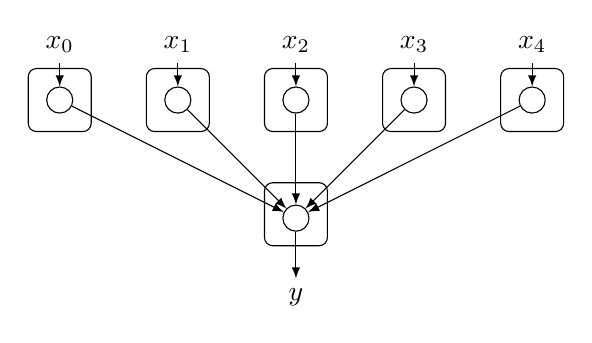
\begin{tikzpicture}

    % Draw inputs.
    \node (i_0) at (-3, 0.7) {$x_0$};
    \node (i_1) at (-1.5, 0.7) {$x_1$};
    \node (i_2) at (0, 0.7) {$x_2$};
    \node (i_3) at (1.5, 0.7) {$x_3$};
    \node (i_4) at (3, 0.7) {$x_4$};


    % Draw the input neurons.
    \node[circle, minimum size=0.2cm, thin, draw=black] (1) at (-3,0) {};
    \node[circle, minimum size=0.2cm, thin, draw=black] (2) at (-1.5,0) {};
    \node[circle, minimum size=0.2cm, thin, draw=black] (3) at (0,0) {};
    \node[circle, minimum size=0.2cm, thin, draw=black] (4) at (1.5,0) {};
    \node[circle, minimum size=0.2cm, thin, draw=black] (5) at (3,0) {};

    % Draw the output neuron.
    \node[circle, minimum size=0.2cm, thin, draw=black] (6) at (0, -1.5) {};

    % Draw output.
    \node (y) at (0, -2.5) {$y$};

    % Draw the lines.
    % X -> Input.
    \draw[->] (i_0) -- (1);
    \draw[->] (i_1) -- (2);
    \draw[->] (i_2) -- (3);
    \draw[->] (i_3) -- (4);
    \draw[->] (i_4) -- (5);
    % Input -> Output.
    \draw[->] (1) -- (6);
    \draw[->] (2) -- (6);
    \draw[->] (3) -- (6);
    \draw[->] (4) -- (6);
    \draw[->] (5) -- (6);
    % Output.
    \draw[->] (6) -- (y);

    % Draw the nodes.
    \draw[rounded corners=3pt] (-3.4,0.4) rectangle ++(0.8,-0.8);
    \draw[rounded corners=3pt] (-1.9,0.4) rectangle ++(0.8,-0.8);
    \draw[rounded corners=3pt] (-0.4,0.4) rectangle ++(0.8,-0.8);
    \draw[rounded corners=3pt] (1.1,0.4) rectangle ++(0.8,-0.8);
    \draw[rounded corners=3pt] (2.6,0.4) rectangle ++(0.8,-0.8);
    \draw[rounded corners=3pt] (-0.4,-1.05) rectangle ++(0.8,-0.8);
  \end{tikzpicture}
  \caption{A perceptron partitioned using the \emph{model parallelism} paradigm. In this approach every input node is responsible for accepting the input $x_i$ from some source, and multiplying the input with the associated weight $w_i$. After the multiplication, the result is sent to the node which is responsible for computing $y$. Of course, this node requires a synchronization mechanism to ensure that the result is consistent. The synchronization mechanism does this by waiting for the results $y$ depends on.}
  \label{fig:introduction_model_parallelism_perceptron}
\end{figure}

\section{Data Parallelism}
\label{sec:intro_data_parallelism}

Data parallelism is an inherently different methodology of optimizing parameters. As stated above, it is a technique to \emph{parallelize gradient descent}, and thereby reducing the overal training time of a model. In essence, data parallelism achieves this by having $n$ workers optimizing a central model, and at the same time, processing $n$ different shards (partitions) of the dataset in parallel over multiple workers\footnote{As stated in Section~\ref{sec:motivation}, a worker is a process on a single machine. However, it is possible that multiple workers share the same machine. Nevertheless, one could construct the distribution mechanism (even manually) in such a way every worker will be placed on a different machine.}. The workers are coordinated in such a way that they optimize the parametrization of a central model, which we denote by $\tilde{\theta}_t$. The coordination mechanism of the workers can be implemented in many different ways. Nevertheless, a popular approach to coordinate workers in their task to optimize the central objective, is to employ a centralized \emph{Parameter Server} (PS). The sole responsibility of the parameter server is to aggregate model updates coming from the workers (\emph{worker commits}), and to handle parameter requests (\emph{worker pulls}). In general, there are several approaches towards data parallelism, where some of which do not require a parameter server. However, all approaches can be categorized into two main groups, i.e., \emph{Synchronous Data Parallelism}, and \emph{Asynchronous Data Parallelism}.\\

\emph{Synchronous Data Parallelism} can be usually identified by the presence of one or multiple locking mechanisms. As in Software Engineering, the purpose of these locking mechanisms is to preserve the consistancy of the state of a model. As an example, let us consider mini-batch parallelism in Figure~\ref{fig:minibatch_data_parallelism} for a moment. Despite it is trivial to implement locally, one could view mini-batch parallelism as an instance of synchronous data parallelism. First and foremost, mini-batch parallelism is a data parallel technique because we split the mini-batch into several partitions where every partition is consumed by its own worker to produce the sum of the gradients, or \emph{accumulated gradient}, as a result. Finally, mini-batch parallelism is synchronous in nature because in order to compute $\theta_{t+1}$, we need to obtain the averaged gradients $\frac{\sum_i \nabla_\theta \mathcal{L}(\theta_t~;~\textbf{x}_i~;~\textbf{y}_i)}{m}$, which is actually the sum of the accumulated gradients of all workers, divided by the number of training instances $m$ in the original mini-batch. As a result, the synchronization barrier is present right before the averaging of the accumulated gradients, since these are the intermediary results we have to wait for before applying a gradient update.

\begin{figure}[H]
  \centering
  % Define database shape.
  \def\database at (#1,#2){
    \draw (#1,#2) ellipse (0.5 and 0.15);
    \draw (#1 - 0.5, #2) -- (#1 - 0.5, #2 - 1);
    \draw (#1 + 0.5, #2) -- (#1 + 0.5, #2 - 1);
    \draw (#1 - 0.5, #2 - 1/3) arc (180:360:0.5 and 0.15);
    \draw (#1 - 0.5, #2 - 2/3) arc (180:360:0.5 and 0.15);
    \draw (#1 - 0.5, #2 - 1) arc (180:360:0.5 and 0.15);
  }
  \def\minibatch at (#1,#2){
    \draw[rounded corners=3pt, draw=black!20, fill=black!10] (#1 - 1.08, #2) rectangle (#1 + 1.08, #2 - 0.8);
    \draw[rounded corners=2pt, draw=blue!35, fill=blue!25, anchor=north] (#1 - 0.25, #2 - 0.4 + 0.25) rectangle (#1 + 0.25, #2 - 0.4 - 0.25);
    \draw[rounded corners=2pt, draw=blue!35, fill=blue!25, anchor=north] (#1 - 0.25 - 0.6, #2 - 0.4 + 0.25) rectangle (#1 + 0.25 - 0.6, #2 - 0.4 - 0.25);
    \draw[rounded corners=2pt, draw=blue!35, fill=blue!25, anchor=north] (#1 - 0.25 + 0.6, #2 - 0.4 + 0.25) rectangle (#1 + 0.25 + 0.6, #2 - 0.4 - 0.25);
    \draw[->] (#1, #2 - 0.9) -- (#1, #2 - 1.5);
  }
  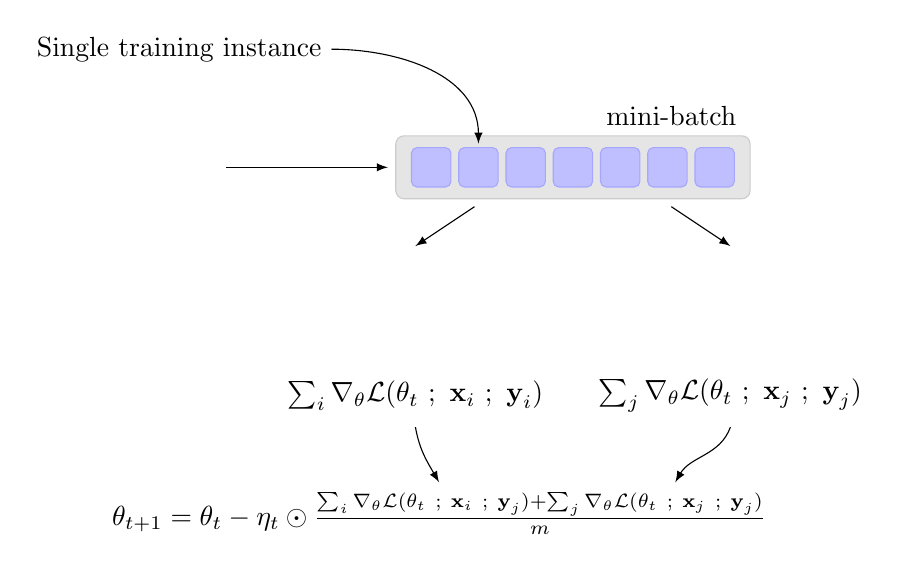
\begin{tikzpicture}
    % Draw the dataset.
    \database at (-5, 0.5);
    \draw[->] (-4.4, 0) -- (-2.35, 0);
    % Draw the minibatch container.
    \draw[rounded corners=3pt, draw=black!20, fill=black!10] (-2.25, 0.4) rectangle (2.25, -0.4);
    % Place the mini-batch label.
    \node at (1.25, 0.65) {mini-batch};
    % Draw the instances inside the minibatch.
    % Center
    \draw[rounded corners=2pt, draw=blue!35, fill=blue!25] (-0.25, 0.25) rectangle (0.25, -0.25);
    % Left
    \draw[rounded corners=2pt, draw=blue!35, fill=blue!25] (-0.25 - 0.6, 0.25) rectangle (0.25 - 0.6, -0.25);
    \draw[rounded corners=2pt, draw=blue!35, fill=blue!25, anchor=north] (-0.25 - 1.2, 0.25) rectangle (0.25 - 1.2, -0.25);
    \draw[rounded corners=2pt, draw=blue!35, fill=blue!25] (-0.25 - 1.8, 0.25) rectangle (0.25 - 1.8, -0.25);
    % Right
    \draw[rounded corners=2pt, draw=blue!35, fill=blue!25] (-0.25 + 0.6, 0.25) rectangle (0.25 + 0.6, -0.25);
    \draw[rounded corners=2pt, draw=blue!35, fill=blue!25] (-0.25 + 1.2, 0.25) rectangle (0.25 + 1.2, -0.25);
    \draw[rounded corners=2pt, draw=blue!35, fill=blue!25] (-0.25 + 1.8, 0.25) rectangle (0.25 + 1.8, -0.25);
    % Draw the training instance description.
    \node at (-5, 1.5) (description) {Single training instance};
    \draw (description) edge[out=0, in=90, ->] (-1.2, 0.3);
    % Draw lines to parallel computation.
    \draw[->] (-1.25, -0.5) -- (-2, -1);
    \draw[->] (1.25, -0.5) -- (2, -1);
    % Draw the minibatches.
    \minibatch at (-2, -1.1);
    \node at (-2, -1.1 - 1.8) {$\sum_i \nabla_\theta \mathcal{L}(\theta_t~;~\textbf{x}_i~;~\textbf{y}_i)$};
    \minibatch at (2, -1.1);
    \node at (2, -1.1 - 1.8) {$\sum_j \nabla_\theta \mathcal{L}(\theta_t~;~\textbf{x}_j~;~\textbf{y}_j)$};
    % Add averaging.
    \draw (2, -3.3) edge[out=-110, in=60, ->] (1.3, -4);
    \draw (-2, -3.3) edge[out=-80, in=120, ->] (-1.7, -4);
    \node at (-1.7, -4.4) {$\theta_{t+1} = \theta_t - \eta_t \odot \frac{\sum_i \nabla_\theta \mathcal{L}(\theta_t~;~\textbf{x}_i~;~\textbf{y}_j) + \sum_j \nabla_\theta \mathcal{L}(\theta_t~;~\textbf{x}_j~;~\textbf{y}_j)}{m}$};
  \end{tikzpicture}
  \caption{Mini-batch parallelism could be viewed as an instance of synchronous data parallelism without a centralized parameter server. Given a mini-batch size of $m$, we split the mini-batch into several partitions, where a specific worker is responsible for the computation of its own partition. The synchronous nature of this approach lies within the aggregation of the computed gradients, i.e., the results of all workers need to be aggregated, and afterwards averaged in order to integrate the current gradient into the model.}
  \label{fig:minibatch_data_parallelism}
\end{figure}

However, consider what happens when the computational resources on your machine are constrained, or even fully utilized? That is, due to the limited amount of available CPU cores (or even GPU's) your parallization of the mini-batch computation doesn't scale very well on your machine. The most straightforward solution would be to purchase more performant hardware, but this is not always possible, not only from a financial perspective, but also from a physical one. An alternative approach would be to solve the problem like a distributed system. In order to make this particular approach work, we need a parameter server to coordinate the workers. Since this still is a synchronous approach, the locking mechanism in this particular case is the parameter server itself, since the parameter server will not be able to send the next parameterization $\theta_{t+1}$ of the model to the workers because the parameter server can only compute the $\theta_{t+1}$ once it received, and processed all accumulated gradients as shown in Figure~\ref{fig:distributed_mini_batch_parallelism}. Yet, if one or multiple machines encouter some unmodeled load, for example, because an other user is running a CPU intensive program, then the synchronization mechanism might actually be a serious bottleneck, because during that time the reserved resources on other machines are not being utilized. This effect becomes even more prominent when the infrastructure is \emph{non-homogeneous}, i.e., multiple machines with different hardware in the same computing cluster cause the workers to be out-of-sync (on top of the unmodeled system behaviour), which in turn results in more waits enforced by the parameter server as it acts as a locking mechanism in synchronous data parallelism.

\begin{figure}[H]
  \centering
  % Define database shape.
  \def\database at (#1,#2){
    \draw (#1,#2) ellipse (0.5 and 0.15);
    \draw (#1 - 0.5, #2) -- (#1 - 0.5, #2 - 1);
    \draw (#1 + 0.5, #2) -- (#1 + 0.5, #2 - 1);
    \draw (#1 - 0.5, #2 - 1/3) arc (180:360:0.5 and 0.15);
    \draw (#1 - 0.5, #2 - 2/3) arc (180:360:0.5 and 0.15);
    \draw (#1 - 0.5, #2 - 1) arc (180:360:0.5 and 0.15);
  }
  % Define datashard shape.
  \def\datashard at (#1,#2){
    \draw (#1,#2) ellipse (0.5 and 0.15);
    \draw (#1 - 0.5, #2) -- (#1 - 0.5, #2 - 1/3);
    \draw (#1 + 0.5, #2) -- (#1 + 0.5, #2 - 1/3);
    \draw (#1 - 0.5, #2 - 1/3) arc (180:360:0.5 and 0.15);
  }
  \def\minibatch at (#1,#2){
    \draw[rounded corners=3pt, draw=black!20, fill=black!10] (#1 - 0.7, #2) rectangle (#1 + 0.7, #2 - 0.8);
    \draw[rounded corners=2pt, draw=blue!35, fill=blue!25, anchor=north] (#1 - 0.55, #2 + 0.25 - 0.4) rectangle (#1 - 0.05, #2 - 0.25 - 0.4);
    \draw[rounded corners=2pt, draw=blue!35, fill=blue!25, anchor=north] (#1 + 0.05, #2 + 0.25 - 0.4) rectangle (#1 + 0.55, #2 - 0.25 - 0.4);
  }
  % Define the neural network shape.
  \def\neuralnet at (#1,#2){
    % Draw node bounding box.
    \draw[rounded corners=3pt] (#1 - 0.7,#2 + 0.5) rectangle ++(1.4,-0.95);
    % Draw fully connected lines.
    \draw[gray] (#1 + 0.25,#2) -- (#1 - 0.375, #2 + 0.25);
    \draw[gray] (#1 + 0.25,#2) -- (#1 - 0.125, #2 + 0.25);
    \draw[gray] (#1 + 0.25,#2) -- (#1 + 0.125, #2 + 0.25);
    \draw[gray] (#1 + 0.25,#2) -- (#1 + 0.375, #2 + 0.25);
    \draw[gray] (#1 + 0.5,#2) -- (#1 - 0.375, #2 + 0.25);
    \draw[gray] (#1 + 0.5,#2) -- (#1 - 0.125, #2 + 0.25);
    \draw[gray] (#1 + 0.5,#2) -- (#1 + 0.125, #2 + 0.25);
    \draw[gray] (#1 + 0.5,#2) -- (#1 + 0.375, #2 + 0.25);
    \draw[gray] (#1,#2) -- (#1 - 0.375, #2 + 0.25);
    \draw[gray] (#1,#2) -- (#1 - 0.125, #2 + 0.25);
    \draw[gray] (#1,#2) -- (#1 + 0.125, #2 + 0.25);
    \draw[gray] (#1,#2) -- (#1 + 0.375, #2 + 0.25);
    \draw[gray] (#1 - 0.25,#2) -- (#1 - 0.375, #2 + 0.25);
    \draw[gray] (#1 - 0.25,#2) -- (#1 - 0.125, #2 + 0.25);
    \draw[gray] (#1 - 0.25,#2) -- (#1 + 0.125, #2 + 0.25);
    \draw[gray] (#1 - 0.25,#2) -- (#1 + 0.375, #2 + 0.25);
    \draw[gray] (#1 - 0.5,#2) -- (#1 - 0.375, #2 + 0.25);
    \draw[gray] (#1 - 0.5,#2) -- (#1 - 0.125, #2 + 0.25);
    \draw[gray] (#1 - 0.5,#2) -- (#1 + 0.125, #2 + 0.25);
    \draw[gray] (#1 - 0.5,#2) -- (#1 + 0.375, #2 + 0.25);
    \draw[gray] (#1 + 0.25,#2) -- (#1 + 0.125, #2 - 0.25);
    \draw[gray] (#1 + 0.25,#2) -- (#1 - 0.125, #2 - 0.25);
    \draw[gray] (#1 + 0.5,#2) -- (#1 + 0.125, #2 - 0.25);
    \draw[gray] (#1 + 0.5,#2) -- (#1 - 0.125, #2 - 0.25);
    \draw[gray] (#1,#2) -- (#1 + 0.125, #2 - 0.25);
    \draw[gray] (#1,#2) -- (#1 - 0.125, #2 - 0.25);
    \draw[gray] (#1 - 0.25,#2) -- (#1 + 0.125, #2 - 0.25);
    \draw[gray] (#1 - 0.25,#2) -- (#1 - 0.125, #2 - 0.25);
    \draw[gray] (#1 - 0.5,#2) -- (#1 + 0.125, #2 - 0.25);
    \draw[gray] (#1 - 0.5,#2) -- (#1 - 0.125, #2 - 0.25);
    % Define input layer.
    \draw[fill=white] (#1 - 0.375,#2 + 0.25) circle (1pt);
    \draw[fill=white] (#1 - 0.125,#2 + 0.25) circle (1pt);
    \draw[fill=white] (#1 + 0.125,#2 + 0.25) circle (1pt);
    \draw[fill=white] (#1 + 0.375,#2 + 0.25) circle (1pt);
    % Define hidden layer.
    \draw[fill=white] (#1 - 0.5,#2) circle (1pt);
    \draw[fill=white] (#1 - 0.25,#2) circle (1pt);
    \draw[fill=white] (#1,#2) circle (1pt);
    \draw[fill=white] (#1 + 0.25,#2) circle (1pt);
    \draw[fill=white] (#1 + 0.5,#2) circle (1pt);
    % Define output layer.
    \draw[fill=white] (#1 - 0.125,#2 - 0.25) circle (1pt);
    \draw[fill=white] (#1 + 0.125,#2 - 0.25) circle (1pt);
  }
  \def\neuralnetclean at (#1,#2){
    \draw[gray] (#1 + 0.25,#2) -- (#1 - 0.375, #2 + 0.25);
    \draw[gray] (#1 + 0.25,#2) -- (#1 - 0.125, #2 + 0.25);
    \draw[gray] (#1 + 0.25,#2) -- (#1 + 0.125, #2 + 0.25);
    \draw[gray] (#1 + 0.25,#2) -- (#1 + 0.375, #2 + 0.25);
    \draw[gray] (#1 + 0.5,#2) -- (#1 - 0.375, #2 + 0.25);
    \draw[gray] (#1 + 0.5,#2) -- (#1 - 0.125, #2 + 0.25);
    \draw[gray] (#1 + 0.5,#2) -- (#1 + 0.125, #2 + 0.25);
    \draw[gray] (#1 + 0.5,#2) -- (#1 + 0.375, #2 + 0.25);
    \draw[gray] (#1,#2) -- (#1 - 0.375, #2 + 0.25);
    \draw[gray] (#1,#2) -- (#1 - 0.125, #2 + 0.25);
    \draw[gray] (#1,#2) -- (#1 + 0.125, #2 + 0.25);
    \draw[gray] (#1,#2) -- (#1 + 0.375, #2 + 0.25);
    \draw[gray] (#1 - 0.25,#2) -- (#1 - 0.375, #2 + 0.25);
    \draw[gray] (#1 - 0.25,#2) -- (#1 - 0.125, #2 + 0.25);
    \draw[gray] (#1 - 0.25,#2) -- (#1 + 0.125, #2 + 0.25);
    \draw[gray] (#1 - 0.25,#2) -- (#1 + 0.375, #2 + 0.25);
    \draw[gray] (#1 - 0.5,#2) -- (#1 - 0.375, #2 + 0.25);
    \draw[gray] (#1 - 0.5,#2) -- (#1 - 0.125, #2 + 0.25);
    \draw[gray] (#1 - 0.5,#2) -- (#1 + 0.125, #2 + 0.25);
    \draw[gray] (#1 - 0.5,#2) -- (#1 + 0.375, #2 + 0.25);
    \draw[gray] (#1 + 0.25,#2) -- (#1 + 0.125, #2 - 0.25);
    \draw[gray] (#1 + 0.25,#2) -- (#1 - 0.125, #2 - 0.25);
    \draw[gray] (#1 + 0.5,#2) -- (#1 + 0.125, #2 - 0.25);
    \draw[gray] (#1 + 0.5,#2) -- (#1 - 0.125, #2 - 0.25);
    \draw[gray] (#1,#2) -- (#1 + 0.125, #2 - 0.25);
    \draw[gray] (#1,#2) -- (#1 - 0.125, #2 - 0.25);
    \draw[gray] (#1 - 0.25,#2) -- (#1 + 0.125, #2 - 0.25);
    \draw[gray] (#1 - 0.25,#2) -- (#1 - 0.125, #2 - 0.25);
    \draw[gray] (#1 - 0.5,#2) -- (#1 + 0.125, #2 - 0.25);
v    \draw[gray] (#1 - 0.5,#2) -- (#1 - 0.125, #2 - 0.25);
    % Define input layer.
    \draw[fill=white] (#1 - 0.375,#2 + 0.25) circle (1pt);
    \draw[fill=white] (#1 - 0.125,#2 + 0.25) circle (1pt);
    \draw[fill=white] (#1 + 0.125,#2 + 0.25) circle (1pt);
    \draw[fill=white] (#1 + 0.375,#2 + 0.25) circle (1pt);
    % Define hidden layer.
    \draw[fill=white] (#1 - 0.5,#2) circle (1pt);
    \draw[fill=white] (#1 - 0.25,#2) circle (1pt);
    \draw[fill=white] (#1,#2) circle (1pt);
    \draw[fill=white] (#1 + 0.25,#2) circle (1pt);
    \draw[fill=white] (#1 + 0.5,#2) circle (1pt);
    % Define output layer.
    \draw[fill=white] (#1 - 0.125,#2 - 0.25) circle (1pt);
    \draw[fill=white] (#1 + 0.125,#2 - 0.25) circle (1pt);
  }
  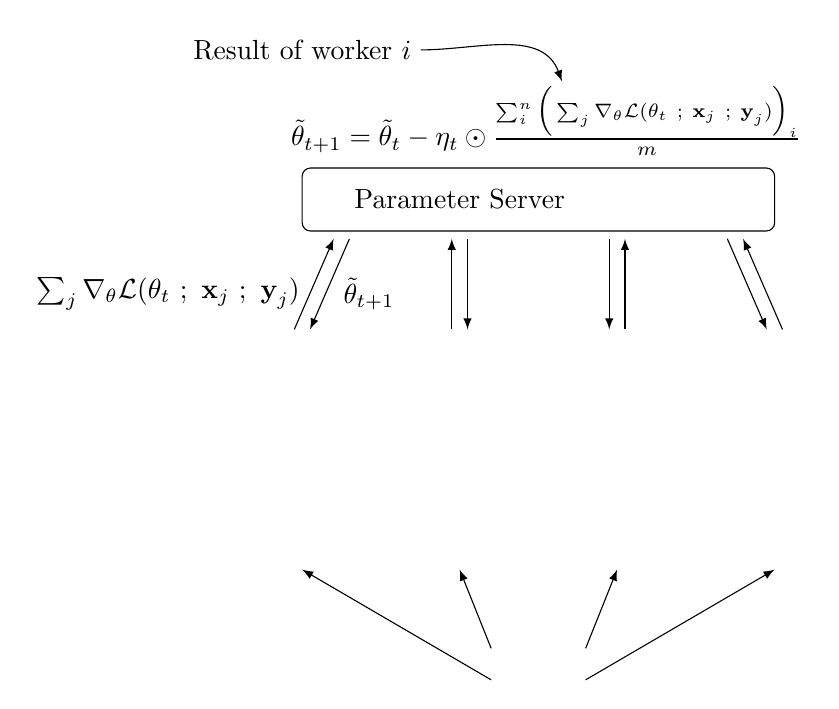
\begin{tikzpicture}
    \database at (0,-1);
    \draw[->] (-0.6,-1.5) -- (-3, -0.1);
    \draw[->] (-0.6,-1.1) -- (-1, -0.1);
    \draw[->] (0.6,-1.1) -- (1, -0.1);
    \draw[->] (0.6,-1.5) -- (3, -0.1);
    \datashard at (-3,0.6);
    \datashard at (-1,0.6);
    \datashard at (1,0.6);
    \datashard at (3,0.6);
    \minibatch at (-3, 1.7);
    \minibatch at (-1, 1.7);
    \minibatch at (1, 1.7);
    \minibatch at (3, 1.7);
    \neuralnet at (3,2.35);
    \neuralnet at (1,2.35);
    \neuralnet at (-1,2.35);
    \neuralnet at (-3,2.35);
    % Draw the parameter server.
    \draw[rounded corners=3pt] (-3, 5) rectangle ++(6,-0.8);
    \node (pslabel) at (-1, 4.6) {Parameter Server};
    \node (psequation) at (0.1, 5.6) {$\tilde{\theta}_{t+1} = \tilde{\theta}_t - \eta_t \odot \frac{\sum_i^n \Big( \sum_j \nabla_\theta \mathcal{L}(\theta_t~;~\textbf{x}_j~;~\textbf{y}_j) \Big)_i}{m}$};
    \node (description) at (-3, 6.5) {Result of worker $i$};
    \draw (description) edge[out=0, in=110, ->] (0.3, 6.1);
    % Draw the lines.
    \neuralnetclean at (1.8, 4.6);
    \draw[->] (-3.1, 2.95) -- (-2.6, 4.1);
    \draw[<-] (-2.9, 2.95) -- (-2.4, 4.1);
    \draw[->] (-1.1, 2.95) -- (-1.1, 4.1);
    \draw[<-] (-0.9, 2.95) -- (-0.9, 4.1);
    \draw[->] (1.1, 2.95) -- (1.1, 4.1);
    \draw[<-] (0.9, 2.95) -- (0.9, 4.1);
    \draw[->] (3.1, 2.95) -- (2.6, 4.1);
    \draw[<-] (2.9, 2.95) -- (2.4, 4.1);
    % Draw the labels.
    \node (commit) at (-2.15, 3.4) {$\tilde{\theta}_{t+1}$};
    \node (pull) at (-4.7, 3.4) {$\sum_j \nabla_\theta \mathcal{L}(\theta_t~;~\textbf{x}_j~;~\textbf{y}_j)$};
    % More labels.
  \end{tikzpicture}
  \caption{Distributed mini-batch data parallelism with $n$ parallel workers, with a total mini-batch size of $m$. At the start, the data is split into $n$ partitions, and all workers get a copy of the central model with parameterization $\tilde{\theta}_0$. When the training starts, every worker $i$ computes the accumulated gradient $\sum_j \nabla_\theta \mathcal{L}(\theta_t~;~\textbf{x}_j~;~\textbf{y}_j)$ based on its part of the mini-batch, which is then \emph{commited} (send) to the parameter server. After the parameter server receives all accumulated gradients, it averages them, and then applies the batched gradient to the model in order to produce $\tilde{\theta}_{t+1}$. After the new parametrization is available, the workers will be able to \emph{pull} (download) $\tilde{\theta}_{t+1}$, and repeat the procedure described above.}
  \label{fig:distributed_mini_batch_parallelism}
\end{figure}

This of course begs the question, \emph{can we eliminate the need for a locking mechanism to prevent unnecessary waits of the workers}? There are some significant initial counter-arguments against removing the synchronization barrier. The most profound issue by removing the synchronization barrier, and thus obtaining \emph{Asynchronous Data Parallelism}, is that the parameter server will incorperate gradients using a simple queuing model (FIFO) based on older parameterizations of the central variable, as shown in Figure~\ref{fig:intro_asyn_data_parallelism}.

\begin{figure}[H]
  \centering
  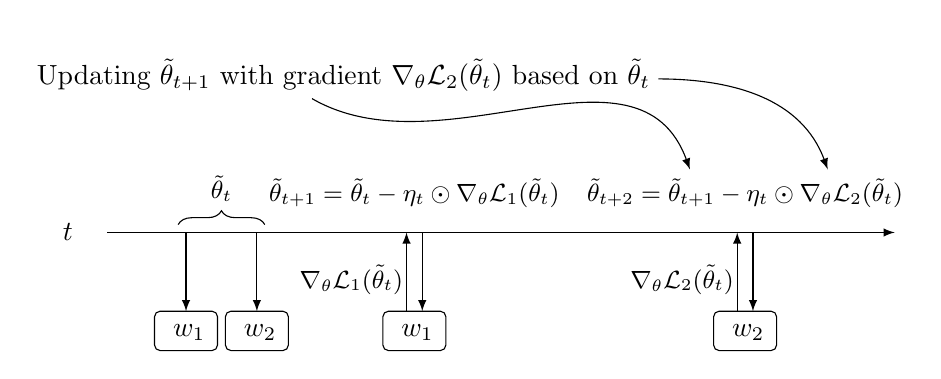
\begin{tikzpicture}
    % Draw the timeline.
    \node at (-5.5, 0) {$t$};
    \draw[->] (-5, 0) -- (5, 0);

    % Draw the first pull of the workers.
    \draw[->] (-4, 0) -- (-4, -1);
    \draw[->] (-3.1, 0) -- (-3.1, -1);
    \draw[rounded corners=2pt] (-4.4, -1) rectangle (-3.6, -1.5) node[pos=.55] {$w_1$};
    \draw[rounded corners=2pt] (-3.5, -1) rectangle (-2.7, -1.5) node[pos=.55] {$w_2$};
    % Draw initial pull decoration.
    \draw [decorate,decoration={brace,amplitude=5pt}]
    (-4.1, 0.1) -- (-3, 0.1) node [black,midway,yshift=13pt] {\small $\tilde{\theta}_t$};

    % Draw first commit and pull.
    \draw[->] (-1, 0) --(-1, -1);
    \draw[<-] (-1.2, 0) -- (-1.2, -1);
    \node at (-1.9, -0.6) {\small $\nabla_\theta \mathcal{L}_1(\tilde{\theta}_t)$};
    \draw[rounded corners=2pt] (-1.1 - 0.4, -1) rectangle (-1.1 + 0.4, -1.5) node[pos=.55] {$w_1$};
    \node at (-1.1, 0.5) {\small $\tilde{\theta}_{t+1} = \tilde{\theta}_t - \eta_t \odot \nabla_\theta \mathcal{L}_1(\tilde{\theta}_t)$};

    % Draw second commit and pull.
    \draw[<-] (3, 0) --(3, -1);
    \draw[->] (3.2, 0) -- (3.2, -1);
    \node at (2.3, -0.6) {\small $\nabla_\theta \mathcal{L}_2(\tilde{\theta}_t)$};
    \draw[rounded corners=2pt] (3.1 - 0.4, -1) rectangle (3.1 + 0.4, -1.5) node[pos=.55] {$w_2$};
    \node at (3.1, 0.5) {\small $\tilde{\theta}_{t+2} = \tilde{\theta}_{t+1} - \eta_t \odot \nabla_\theta \mathcal{L}_2(\tilde{\theta}_t)$};

    % Write description.
    \node at (-2, 2) {Updating $\tilde{\theta}_{t+1}$ with gradient $\nabla_\theta \mathcal{L}_2(\tilde{\theta}_t)$ based on $\tilde{\theta}_t$};
    \draw (-2.4, 1.7) edge[out=-30, in=110, ->] (2.4, 0.8);
    \draw (2, 1.95) edge[out=0, in=110, ->] (4.15, 0.8);
  \end{tikzpicture}
  \caption{In Asynchronous Data Parallelism workers compute and commit gradients to the parameter server asynchronously. This has as a side-effect that some workers are computing, and thus committing, gradients based on old values. These gradients are called \emph{stale gradients} in literature. In this particular example there are 2 workers $w_1$, and $w_2$. At the start optimization process, the pull the most recent parameterization from the parameter server $\tilde{\theta}_t$. Now all workers start computing the gradients asynchronously based on the pulled parametrization. However, since the parameter server incorperates gradients into the center variable asynchronously as a simple queuing (FIFO) model, other workers will update the center variable with gradients based on an older value, as shown in the figure above. Finally, assuming that the computing cluster is homogeneous, we can derive from this figure that the expected staleness of a gradient update is $\mathbf{E}[\tau] = (n - 1)$.}
  \label{fig:intro_asyn_data_parallelism}
\end{figure}

However, experiments have shown that removing the synchronization barrier actually allows models to converge~\cite{dean2012large, zhang2015deep, hadjis2016omnivore}, even when most workers update the central variable using a gradient based on an outdated parameterization of the central variable. An other issue, which only has been formalized recently, is \emph{Implicit Momentum} or \emph{Asynchrony Induced Momentum}~\cite{implicitmomentum}. The main reasoning behind implicit momentum, which will be discussed in detail in Section~\ref{sec:implicit_momentum}, is based on a very simple but powerful idea. The idea states that \emph{memory arizes from asynchrony}. Intuitively, this implies that ``memory'' of previous gradients is preserved due to \emph{stale gradient} updates. This can be observed directly from Figure~\ref{fig:intro_asyn_data_parallelism}, where the update of $w_2$ is actually updating the central variable with a gradient identical to $\nabla_\theta \mathcal{L}_1(\tilde{\theta}_t)$ if we assume that both workers computed the gradient based on the same input data. This is a clear indication that asynchronous data parallelism is \emph{implicitly} (because of the asynchronous nature of the approach) adding \emph{momentum} which is proportional to the number of workers, since adding more workers actually \emph{adds} more ``memory'' about previous parameterizations. The authors formalize this by probabilistically estimating the expected change between $\tilde{\theta}_{t+1}$ and $\tilde{\theta}_t$. Using some additional additional assumptions, such as the expected staleness $\mathbf{E}[\tau] = (n - 1)$, and geometrically distributed staleness, the authors are able to formalize the expected update in an asynchronous setting between update $t$ and $t + 1$, which is shown in Equation~\ref{eq:implicit_momentum}.\\

\begin{equation}
  \label{eq:implicit_momentum}
  \mathbf{E}[\tilde{\theta}_{t+1} - \tilde{\theta}_t] = \Bigg( 1 - \frac{1}{n} \Bigg) \mathbf{E}[\tilde{\theta}_t - \tilde{\theta}_{t-1}] - \frac{\eta}{n} \mathbf{E} \nabla_\theta \mathcal{L}(\tilde{\theta}_t~;~\textbf{x}~;~\textbf{y})
\end{equation}

Using Equation~\ref{eq:implicit_momentum}, we can immediatly derrive the term which describes the implicit momentum induced by asynchrony, which is $\big(1 - \frac{1}{n}\big)$. This result actually suggests that there is a limit to asynchronous optimization: since every problem has some optimal momentum term, which implies that there is an optimal number of asynchronous workers for a specific problem. In order to push the limits of asynchronous optimization, the authors propose various techniques to reduce the abundant amount of implicit momentum. One approach is to apply a \emph{grid-search} to find the optimal hyperparameterization for a given epoch, this also includes the number of workers. Despite that this technique finds the optimal hyperparameterization for a given epoch, the disadvantage is that after every fixed number of iterations, a grid-search of the hyperparameters has to be performed to ensure (optimal) convergence. This is actually in accordance with training in non-data parallel settings, where one starts with a smaller momentum hyperparameter because the gradients at the start will be relatively large compared to the gradients near an optimum, where usually one benifits from a larger momentum hyperparameter. From this intuition we can actually deduce that when the gradient updates are large compared to the gradients close to an optimum, an optimizer does not benifit from high parallelism because the workers are committing a gradient which was based on a parametrization which is ``far'' from the current central variable, thus obtaining implicit momentum. Furthermore, one could eliminate the need for the gridsearch by constructing a distributed optimization scheme which is based on the following idea: \emph{workers only contribute efficiently to the central objective when they commit gradients which are based on variables close to the central variable}. This implies that when there is a high amount of parallelism, only the gradient updates which are based on variables close to the \emph{current} central variable should matter. This intuition is strengthened in Figure~\ref{fig:async_momentum}.

\begin{figure}[H]
  \centering
  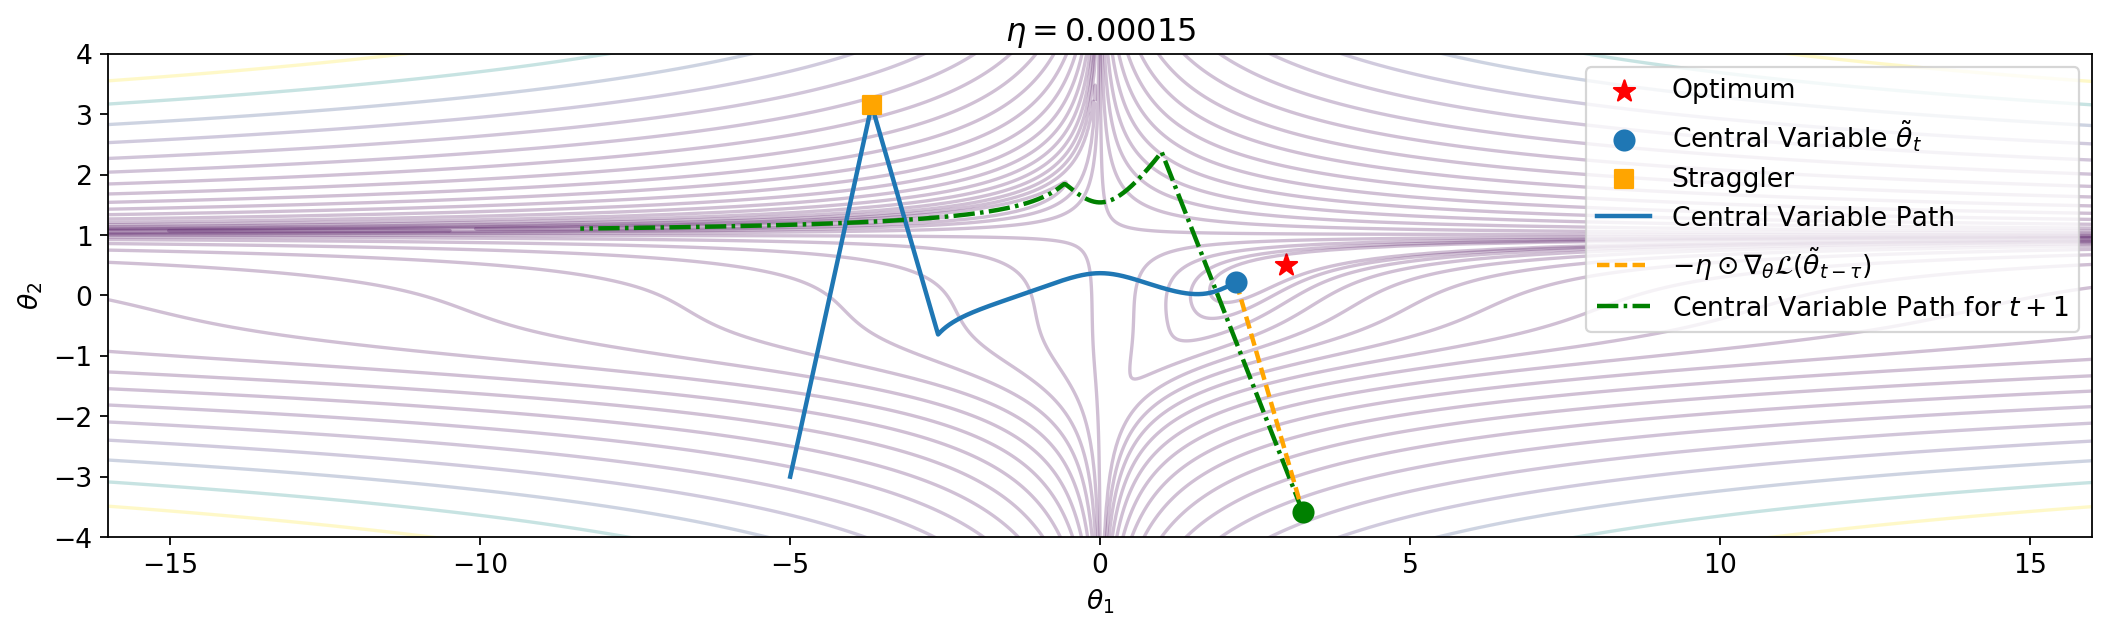
\includegraphics[width=\textwidth]{resources/images/async_straggler}
  \caption{TODO}
  \label{fig:async_momentum}
\end{figure}

One could of course argue, why not use a smaller number of workers since you are annealing the gradients which are based on non-local variables anyway, thus wasting computational resources on those machines? This is certainly a valid argument. However, let us first consider the hyperparameter grid-search approach suggested by~\cite{implicitmomentum}. As mentioned above, despite the fact that the grid-search technique will find the optimal hyperparameters for the current parameterization, it doesn't mean that these hyperparameters are still optimal during the duration of the training process. Furthermore, to actually obtain the optimal hyperparameters, some certain amount of time needs to be spent in order to find them. This is actually quite problematic, since time is an important factor in data parallel approaches because it is actually the factor we wish to reduce. In our approach, which will be discussed extensively in Chapter~\ref{chapter:asynchronous_distributed_adaptive_gradients}, this is not the case since the gradients will be annealed dynamically based on the curvature of the error space and current parametrization of the central variable, i.e., there is no need for a hyperparameter grid-search.\\

In order to formalize the main concept of data parallelism, let us assume we have a dataset $D$, which contains our training data, and that we are able to distribute dataset $D$ over $n$ different workers $\mathcal{W} = \{w_1, \ldots, w_n\}$. Where every worker $w_i \in \mathcal{W}$ holds a copy of the central model, thus, a copy of the parameterization of the central model $\tilde{\theta}_0$. Furthermore, we denote the parametrization of a particular worker $k$ at time $t$ by $\theta_t^k$. Of course, if a worker wants to contribute to the optimization of the central model, the worker needs to be able to relay update information and retrieve the most recent parameterization of the central model. This is done by instantiating a parameter server, where workers will be able to \emph{commit} their updates, and \emph{pull} the most recent parameterization of the central model. The parameterization of the central model is called the \emph{central variable}, which we denote by $\tilde{\theta}_t$. In the final preperation step, before the actual training starts, $\mathcal{D}$ will be split into roughly $n$ equally sized partitions $\mathcal{P} = \{p_1, \ldots, p_n\}$, where $\left\vert{p_i}\right\vert \approx \frac{1}{\left\vert{\mathcal{D}}\right\vert}$, and where $p_i$ will be assigned to the corresponding worker $w_i$.\\

\begin{figure}[H]
  \centering
  % Define database shape.
  \def\database at (#1,#2){
    \draw (#1,#2) ellipse (0.5 and 0.15);
    \draw (#1 - 0.5, #2) -- (#1 - 0.5, #2 - 1);
    \draw (#1 + 0.5, #2) -- (#1 + 0.5, #2 - 1);
    \draw (#1 - 0.5, #2 - 1/3) arc (180:360:0.5 and 0.15);
    \draw (#1 - 0.5, #2 - 2/3) arc (180:360:0.5 and 0.15);
    \draw (#1 - 0.5, #2 - 1) arc (180:360:0.5 and 0.15);
  }
  % Define datashard shape.
  \def\datashard at (#1,#2){
    \draw (#1,#2) ellipse (0.5 and 0.15);
    \draw (#1 - 0.5, #2) -- (#1 - 0.5, #2 - 1/3);
    \draw (#1 + 0.5, #2) -- (#1 + 0.5, #2 - 1/3);
    \draw (#1 - 0.5, #2 - 1/3) arc (180:360:0.5 and 0.15);
  }
  % Define the neural network shape.
  \def\neuralnet at (#1,#2){
    % Draw node bounding box.
    \draw[rounded corners=3pt] (#1 - 0.7,#2 + 0.5) rectangle ++(1.4,-0.95);
    % Draw fully connected lines.
    \draw[gray] (#1 + 0.25,#2) -- (#1 - 0.375, #2 + 0.25);
    \draw[gray] (#1 + 0.25,#2) -- (#1 - 0.125, #2 + 0.25);
    \draw[gray] (#1 + 0.25,#2) -- (#1 + 0.125, #2 + 0.25);
    \draw[gray] (#1 + 0.25,#2) -- (#1 + 0.375, #2 + 0.25);
    \draw[gray] (#1 + 0.5,#2) -- (#1 - 0.375, #2 + 0.25);
    \draw[gray] (#1 + 0.5,#2) -- (#1 - 0.125, #2 + 0.25);
    \draw[gray] (#1 + 0.5,#2) -- (#1 + 0.125, #2 + 0.25);
    \draw[gray] (#1 + 0.5,#2) -- (#1 + 0.375, #2 + 0.25);
    \draw[gray] (#1,#2) -- (#1 - 0.375, #2 + 0.25);
    \draw[gray] (#1,#2) -- (#1 - 0.125, #2 + 0.25);
    \draw[gray] (#1,#2) -- (#1 + 0.125, #2 + 0.25);
    \draw[gray] (#1,#2) -- (#1 + 0.375, #2 + 0.25);
    \draw[gray] (#1 - 0.25,#2) -- (#1 - 0.375, #2 + 0.25);
    \draw[gray] (#1 - 0.25,#2) -- (#1 - 0.125, #2 + 0.25);
    \draw[gray] (#1 - 0.25,#2) -- (#1 + 0.125, #2 + 0.25);
    \draw[gray] (#1 - 0.25,#2) -- (#1 + 0.375, #2 + 0.25);
    \draw[gray] (#1 - 0.5,#2) -- (#1 - 0.375, #2 + 0.25);
    \draw[gray] (#1 - 0.5,#2) -- (#1 - 0.125, #2 + 0.25);
    \draw[gray] (#1 - 0.5,#2) -- (#1 + 0.125, #2 + 0.25);
    \draw[gray] (#1 - 0.5,#2) -- (#1 + 0.375, #2 + 0.25);
    \draw[gray] (#1 + 0.25,#2) -- (#1 + 0.125, #2 - 0.25);
    \draw[gray] (#1 + 0.25,#2) -- (#1 - 0.125, #2 - 0.25);
    \draw[gray] (#1 + 0.5,#2) -- (#1 + 0.125, #2 - 0.25);
    \draw[gray] (#1 + 0.5,#2) -- (#1 - 0.125, #2 - 0.25);
    \draw[gray] (#1,#2) -- (#1 + 0.125, #2 - 0.25);
    \draw[gray] (#1,#2) -- (#1 - 0.125, #2 - 0.25);
    \draw[gray] (#1 - 0.25,#2) -- (#1 + 0.125, #2 - 0.25);
    \draw[gray] (#1 - 0.25,#2) -- (#1 - 0.125, #2 - 0.25);
    \draw[gray] (#1 - 0.5,#2) -- (#1 + 0.125, #2 - 0.25);
    \draw[gray] (#1 - 0.5,#2) -- (#1 - 0.125, #2 - 0.25);
    % Define input layer.
    \draw[fill=white] (#1 - 0.375,#2 + 0.25) circle (1pt);
    \draw[fill=white] (#1 - 0.125,#2 + 0.25) circle (1pt);
    \draw[fill=white] (#1 + 0.125,#2 + 0.25) circle (1pt);
    \draw[fill=white] (#1 + 0.375,#2 + 0.25) circle (1pt);
    % Define hidden layer.
    \draw[fill=white] (#1 - 0.5,#2) circle (1pt);
    \draw[fill=white] (#1 - 0.25,#2) circle (1pt);
    \draw[fill=white] (#1,#2) circle (1pt);
    \draw[fill=white] (#1 + 0.25,#2) circle (1pt);
    \draw[fill=white] (#1 + 0.5,#2) circle (1pt);
    % Define output layer.
    \draw[fill=white] (#1 - 0.125,#2 - 0.25) circle (1pt);
    \draw[fill=white] (#1 + 0.125,#2 - 0.25) circle (1pt);
  }
  \def\neuralnetclean at (#1,#2){
    \draw[gray] (#1 + 0.25,#2) -- (#1 - 0.375, #2 + 0.25);
    \draw[gray] (#1 + 0.25,#2) -- (#1 - 0.125, #2 + 0.25);
    \draw[gray] (#1 + 0.25,#2) -- (#1 + 0.125, #2 + 0.25);
    \draw[gray] (#1 + 0.25,#2) -- (#1 + 0.375, #2 + 0.25);
    \draw[gray] (#1 + 0.5,#2) -- (#1 - 0.375, #2 + 0.25);
    \draw[gray] (#1 + 0.5,#2) -- (#1 - 0.125, #2 + 0.25);
    \draw[gray] (#1 + 0.5,#2) -- (#1 + 0.125, #2 + 0.25);
    \draw[gray] (#1 + 0.5,#2) -- (#1 + 0.375, #2 + 0.25);
    \draw[gray] (#1,#2) -- (#1 - 0.375, #2 + 0.25);
    \draw[gray] (#1,#2) -- (#1 - 0.125, #2 + 0.25);
    \draw[gray] (#1,#2) -- (#1 + 0.125, #2 + 0.25);
    \draw[gray] (#1,#2) -- (#1 + 0.375, #2 + 0.25);
    \draw[gray] (#1 - 0.25,#2) -- (#1 - 0.375, #2 + 0.25);
    \draw[gray] (#1 - 0.25,#2) -- (#1 - 0.125, #2 + 0.25);
    \draw[gray] (#1 - 0.25,#2) -- (#1 + 0.125, #2 + 0.25);
    \draw[gray] (#1 - 0.25,#2) -- (#1 + 0.375, #2 + 0.25);
    \draw[gray] (#1 - 0.5,#2) -- (#1 - 0.375, #2 + 0.25);
    \draw[gray] (#1 - 0.5,#2) -- (#1 - 0.125, #2 + 0.25);
    \draw[gray] (#1 - 0.5,#2) -- (#1 + 0.125, #2 + 0.25);
    \draw[gray] (#1 - 0.5,#2) -- (#1 + 0.375, #2 + 0.25);
    \draw[gray] (#1 + 0.25,#2) -- (#1 + 0.125, #2 - 0.25);
    \draw[gray] (#1 + 0.25,#2) -- (#1 - 0.125, #2 - 0.25);
    \draw[gray] (#1 + 0.5,#2) -- (#1 + 0.125, #2 - 0.25);
    \draw[gray] (#1 + 0.5,#2) -- (#1 - 0.125, #2 - 0.25);
    \draw[gray] (#1,#2) -- (#1 + 0.125, #2 - 0.25);
    \draw[gray] (#1,#2) -- (#1 - 0.125, #2 - 0.25);
    \draw[gray] (#1 - 0.25,#2) -- (#1 + 0.125, #2 - 0.25);
    \draw[gray] (#1 - 0.25,#2) -- (#1 - 0.125, #2 - 0.25);
    \draw[gray] (#1 - 0.5,#2) -- (#1 + 0.125, #2 - 0.25);
v    \draw[gray] (#1 - 0.5,#2) -- (#1 - 0.125, #2 - 0.25);
    % Define input layer.
    \draw[fill=white] (#1 - 0.375,#2 + 0.25) circle (1pt);
    \draw[fill=white] (#1 - 0.125,#2 + 0.25) circle (1pt);
    \draw[fill=white] (#1 + 0.125,#2 + 0.25) circle (1pt);
    \draw[fill=white] (#1 + 0.375,#2 + 0.25) circle (1pt);
    % Define hidden layer.
    \draw[fill=white] (#1 - 0.5,#2) circle (1pt);
    \draw[fill=white] (#1 - 0.25,#2) circle (1pt);
    \draw[fill=white] (#1,#2) circle (1pt);
    \draw[fill=white] (#1 + 0.25,#2) circle (1pt);
    \draw[fill=white] (#1 + 0.5,#2) circle (1pt);
    % Define output layer.
    \draw[fill=white] (#1 - 0.125,#2 - 0.25) circle (1pt);
    \draw[fill=white] (#1 + 0.125,#2 - 0.25) circle (1pt);
  }
  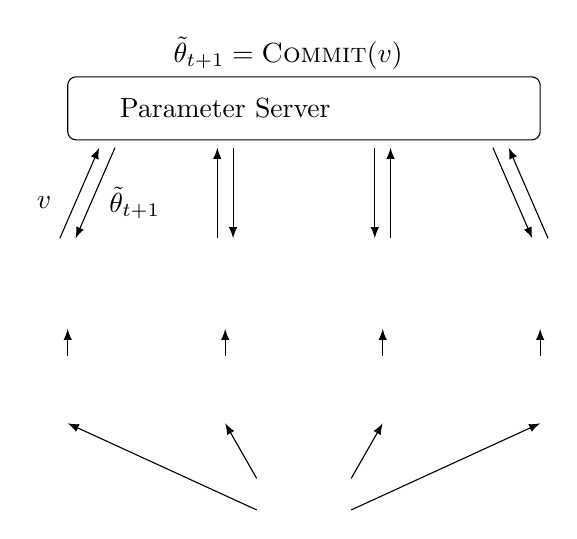
\begin{tikzpicture}
    \database at (0,0);
    \draw[->] (-0.6,-0.5) -- (-3, 0.6);
    \draw[->] (-0.6,-0.1) -- (-1, 0.6);
    \draw[->] (0.6,-0.1) -- (1, 0.6);
    \draw[->] (0.6,-0.5) -- (3, 0.6);
    \datashard at (-3,1.2)
    \datashard at (-1,1.2);
    \datashard at (1,1.2);
    \datashard at (3,1.2);
    \draw[->] (-3, 1.45) -- (-3, 1.8);
    \draw[->] (-1, 1.45) -- (-1, 1.8);
    \draw[->] (1, 1.45) -- (1, 1.8);
    \draw[->] (3, 1.45) -- (3, 1.8);
    \neuralnet at (3,2.35);
    \neuralnet at (1,2.35);
    \neuralnet at (-1,2.35);
    \neuralnet at (-3,2.35);
    % Draw the parameter server.
    \draw[rounded corners=3pt] (-3, 5) rectangle ++(6,-0.8);
    \node (pslabel) at (-1, 4.6) {Parameter Server};
    \node (psequation) at (-0.2, 5.3) {$\tilde{\theta}_{t+1} = \textsc{Commit}(v)$};
    % Draw the lines.
    \neuralnetclean at (1.8, 4.6);
    \draw[->] (-3.1, 2.95) -- (-2.6, 4.1);
    \draw[<-] (-2.9, 2.95) -- (-2.4, 4.1);
    \draw[->] (-1.1, 2.95) -- (-1.1, 4.1);
    \draw[<-] (-0.9, 2.95) -- (-0.9, 4.1);
    \draw[->] (1.1, 2.95) -- (1.1, 4.1);
    \draw[<-] (0.9, 2.95) -- (0.9, 4.1);
    \draw[->] (3.1, 2.95) -- (2.6, 4.1);
    \draw[<-] (2.9, 2.95) -- (2.4, 4.1);
    % Draw the labels.
    \node (commit) at (-2.15, 3.4) {$\tilde{\theta}_{t+1}$};
    \node (pull) at (-3.3, 3.4) {$v$};
    % More labels.
  \end{tikzpicture}
  \caption{Schematic representation of a data parallel approach. In this methodology we spawn $n$ workers (not necessarily on different machines), and assign a data shard (partition) of the dataset to every worker. Using this data shard, a worker $i$ will iterate through all mini-batches to produce a gradient, $\nabla_\theta \mathcal{L}_i(x)$, for every mini-batch $x$. Next, $\nabla_\theta \mathcal{L}_i(x)$ is send to the parameter server, which will incorperate the gradient using an~\textsc{update} mechanism.}
  \label{fig:introduction_data_parallelism_schematic}
\end{figure}

In general, all data parallel approaches share a similar training procedure, i.e., every worker computes some variable which is communicated with the parameter server to update the central model. In most cases, this variable represents some change $\Delta\theta$ which needs to be applied to the central variable $\tilde{\theta}_t$. However, some approaches such as~\cite{zhang2015deep}, actually require that the complete worker parametrization $\theta^k_t$ is sent to the parameter server. To simplify this specific optimizer detail in this chapter, we denote the variable that is sent to the parameter server by $v$.

% Define the general data parallel worker algorithm.
\begin{algorithm}[H]
  \caption{Describes the general optimization procedure of a worker in a data parallel setting. The worker will be identified with a certain index $k$, the other parameter $p_k \in \mathcal{P}$, is the data partition which has been assigned to worker $k$.}
  \label{algo:data_parallelism_worker}
  \begin{algorithmic}[1]
    \Procedure{Worker}{$k$, $p_k$}
    \State $\theta^k_0 \gets \Call{Pull}{ }$
    \State $t \gets 0$
    \While{$\textbf{not}$ converged}
    \State $\textbf{m} \gets \Call{FetchNextMiniBatch}{p_k}$
    \State $\theta^k_{t + 1} \gets \theta^k_t - \eta_t \odot \nabla_\theta \mathcal{L}(\theta^k_t~;~\textbf{m})$ \Comment{Optimization step, could be \cite{kingma2014adam}, or other optimizer.}
    \State $v \gets \Call{PrepareCommit}{ }$
    \State $\Call{Commit}{v}$
    \State $\theta^k_t \gets \Call{Pull}{ }$
    \State $t \gets t + 1$
    \EndWhile
    \EndProcedure
  \end{algorithmic}
\end{algorithm}

% Define the general commit update mechanism.
\begin{algorithm}[H]
  \caption{Intialization and variable handling procedures of a parameter server. Before the distributed optimization starts, the \textsc{IntializeParameterServer} procedure is called to initialize the local parameters, given the parametrization $\theta$ of the specified model. We would like to note that $t$ maintained by the parameter server, is different from the $t$ variable specified in Algorithm~\ref{algo:data_parallelism_worker}.}
  \label{algo:data_parallelism_parameter_server}
  \begin{algorithmic}[1]
    \Procedure{IntializeParameterServer}{$\theta$}
    \State $\tilde{\theta}_0 \gets \theta$
    \State $t \gets 0$
    \EndProcedure
    \State
    \Procedure{Commit}{$v$}
    \State $\tilde{\theta}_{t + 1} \gets \Call{ApplyCommit}{v}$
    \State $t \gets t + 1$
    \EndProcedure
    \State
    \Procedure{Pull}{ }
    \State \Return $\tilde{\theta}_t$
    \EndProcedure
  \end{algorithmic}
\end{algorithm}

\section{Problem Statement}
\label{sec:problem_statement}

TODO

\section{Thesis Outline}
\label{sec:thesis_outline}

TODO

% Chapter on Optimizers.
%
% Developed for my Master Thesis at Maastricht University.
% Based on Eugenio Senes's template at the University of Torino.
%
% By Joeri Hermans (joeri@joerihermans.com)
%
% Released under an MIT license. Share, modify and enjoy, but quote the author!

\chapter{Optimization Algorithms}
\label{chapter:optimization_algorithms}

% Chapter on Distributed Deep Learning.
%
% Developed for my Master Thesis at Maastricht University.
% Based on Eugenio Senes's template at the University of Torino.
%
% By Joeri Hermans (joeri@joerihermans.com)
%
% Released under an MIT license. Share, modify and enjoy, but quote the author!

\chapter{Distributed Deep Learning}
\label{chapter:distributed_deep_learning}

In this chapter, we introduce several concepts and techniques related to Distributed Deep Learning on which this works builts upon. We start in Section~\ref{sec:ddl_introduction} with a recap of all methods and techniques we have discussed in Chapter~\ref{chapter:introduction}. Afterwards, we continue with a discussion of synchronous followed by an examination of asynchronous optimization methods such as \textsc{downpour} and closely related extensions. Furthermore, we address several issues such as \emph{asynchrony induced momentum} which are related to asynchronous optimization. We also consider several approaches which provide a possible solution to these issues.

\section{Introduction}
\label{sec:ddl_introduction}

For all practical applications, Stochastic Gradient Descent (\textsc{sgd}) and derrivatives are the best tools from the numerical optimization toolbox for neural networks. However, applying \textsc{sgd} in its pure form, that is, updating the parameters after evaluating a training sample, is a computationally intensive process. An initial approach for speeding up \textsc{sgd} in terms of convergence with respect to training time was to compute the gradients of several samples, a \emph{mini-batch}, and average them. This approach has several advantages, the first being that a larger mini-batch will result in less noisy updates, as more ``evidence'' of the surrounding error space will provide a better gradient update. The second advantage being the increased computational parallelism, since all sub-gradients (gradients of the training samples in the mini-batch) are based upon the same parametrization of the model. As a result, the parallelization of the gradient computation is quite straightforward. For instance, for every training sample in a mini-batch, one could allocate a thread, a process, or even a different machine (see Figure~\ref{fig:distributed_mini_batch_parallelism}) to compute the gradients in parallel. However, a blocking mechanism is required in order to sum all gradients, average them, and finally update the parametrization of the model. This process is depicted in Figure~\ref{fig:minibatch_data_parallelism}. As discussed in Chapter~\ref{chapter:introduction}, mini-batch parallelism is an instance of \emph{synchronous data parallelism}. Although many synchronous optimization schemes share a similar structure, we discuss other instances of synchronous data parallelism in particular in Section~\ref{sec:synchronous_data_parallelism} since these optimization schemes incorperate gradients and worker parameterizations into the central variable differently compared to mini-batch parallelism.\\

Nevertheless, a significant, but albeit technical issue in synchronous optimization is when a single or multiple workers are slowed down for some reason, e.g., due to high CPU load, or bandwidth consumption, other workers will have to wait before they can continue with step $t + 1$. As a result, the allocated resources are not fully utilized. This particular issue is known in literature as the \emph{straggler} problem. However, this problem can be mitigated with by using a \emph{homogeneous} hardware configuration. For instance, when one would employ 2 different GPU's running at different clock speeds, a \emph{heteregenous} hardware configuration, then the CPU will always have to wait for a particulur GPU since it runs at a lower clock speed causing the complete training procedure to be slowed down\footnote{A chain is only as strong as its weakest link.}. Furthermore, we could argue that there is a limit to synchronous data parallelism because simply \emph{adding more workers to the problem implicitly increases the size of the mini-batch}. As a result, when applying synchronous data parallelism, one is not parallelizing gradient descent in a typical sense, but rather parallelizing the computations within a step. Of course, one could even increase the parallelism within synchronous data parallelism even further by applying model parallelism as dicussed briefly in Section~\ref{sec:intro_model_parallelism}. Nevertheless, while such an implementation is definitly possible, it might be more cost-aware from an economical perspective to just let the model train for a longer period of the compared to actually implementing the training procedure described above. Furthermore, even with if one would implement said training method, there is still a limit to the amount parallelism due to the structure of the computation graph, and communication cost between devices which have to be taken into account. This of course begs the question if it is actually possible to push the limits of asynchrony, and thereby reducing the training time even further. Or from a different perspective, is there a more trivial method besides implementing the above training procedure to reduce the training time.\\

Several approaches~\cite{dean2012large, ho2013more, cipar2013solving, recht2011hogwild, zhang2015deep, louppe2010zealous, jiang2017heterogeneity} have been suggested over the past years which accomplish exactly this. All these methods are instances of \emph{asynchronous data parallelism}, discussed in Section~\ref{sec:intro_data_parallelism}. In contrast to synchronous data parallelism, asynchronous methods can be identified by the \emph{absence} of a blocking mechanism which is present in synchronous data parallelism. Despite the fact that this method resolves the waiting time induced by stragglers, it introduces a closely related but persistent issue. More formally, the \emph{staleness} issue is due to the fact that all $n$ workers update the central variable in an asynchronous fashion. Meaning, from the moment a worker $k$ is done computing an update $\Delta\theta^k$ based upon parameterization of the central variable $\tilde{\theta}_{t}$, it will commit $\Delta\theta^k$ to the parameter server, and afterwards continue with the next mini-batch. Because of this behaviour, it is possible that a number of central variable updates $\tau$ occurred during the time worker $k$ was computing $\Delta\theta^k$. As a result, instead of obtaining $\tilde{\theta}_{t+1}$ by applying $\Delta\theta^k$, worker $k$ is actually applying $\Delta\theta^k$ to $\tilde{\theta}_{t+\tau}$. Which is not ideal, since $\Delta\theta^k$ is based on parametrization $\tilde{\theta}_t$. From~\cite{implicitmomentum} we know that increasing the number of workers actually increases the amount of staleness $\tau$ since $\mathbf{E}[\tau] = (n - 1)$ under a \emph{homogeneous} hardware configuration and a simple queuing model\footnote{With a simple queuing model we intent that updates $\Delta\theta^k$ are incorperated into the central variable in a queuing fashion.}. This result is validated empirically in one of our experiments, shown in Figure~\ref{fig:staleness_distribution}.\\

A side-effect of updating the central variable with stale updates in an asynchronous fashion, is that stale updates carry information about previous states of the central variable. Which is to be expected since worker updates are based on older parameterizations of the central variable. Using this intuition, the authors in~\cite{implicitmomentum} show formally that in a regular asynchronous \textsc{sgd} setting, like \textsc{downpour}, stale updates behave like \emph{momentum}. Furthermore, their formalization can even describe the amount of \emph{implicit momentum}, described in Equation~\ref{eq:implicit_momentum}, which is present in an asynchronous optimization procedure. Furthermore, when applying (Nesterov) momentum in a traditional optimization setting, i.e., sequential parameter updates, one needs to specify the amount of momentum. This is usually denoted by a hyperparameter $\mu$. However, we would like to note that in an asynchronous setting, the hyperparameter $\mu_s$ from Equation~\ref{eq:implicit_momentum}, is not explicitly defined in the optimizer, but arises from the number of asynchronous workers. As a result, Equation~\ref{eq:implicit_momentum} is merely descriptive.

\begin{equation}
  \label{eq:implicit_momentum}
  \mu_s = \Bigg(1 - \frac{1}{n}\Bigg)
\end{equation}

In a previous paragraph we said that there is a limit to mini-batch parallelism, since adding more workers to the problem implicitly increases the size of a mini-batch. However, we observe in Figure~\ref{fig:staleness_distribution} in accordance with~\cite{implicitmomentum}, that there might be a limit to asynchronous optimization as well. However, the authors in~\cite{implicitmomentum} assume that gradients coming from the workers are not adaptive\footnote{Meaning, they are not modified with respect to some (hyper)parameter.}, as can be detucted from their proof. The question begs, can we push asynchronous optimization even further? We answer this question in Chapter~\ref{chapter:accumulated_gradient_normalization}, and Chapter~\ref{chapter:asynchronous_distributed_adaptive_gradients}, by introducing new techniques using a better, and more intuitive understanding of parameter staleness.

\begin{figure}
  \centering
  \begin{subfigure}{.45\textwidth}
    \centering
    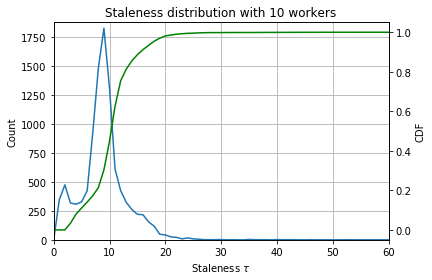
\includegraphics[width=\linewidth]{resources/images/staleness_10}
    \caption{$n = 10$}
    \label{fig:staleness_distribution_10}
  \end{subfigure}
  \begin{subfigure}{.45\textwidth}
     \centering
     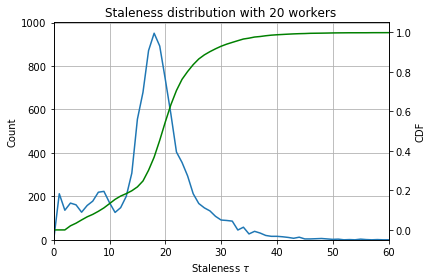
\includegraphics[width=\linewidth]{resources/images/staleness_20}
     \caption{$n = 20$}
    \label{fig:staleness_distribution_20}
  \end{subfigure}
  \begin{subfigure}{.45\textwidth}
     \centering
     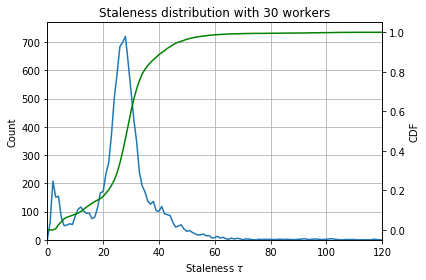
\includegraphics[width=\linewidth]{resources/images/staleness_30}
     \caption{$n = 30$}
     \label{fig:staleness_distribution_30}
  \end{subfigure}
  \begin{subfigure}{.45\textwidth}
     \centering
     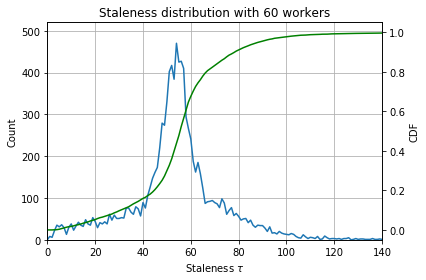
\includegraphics[width=\linewidth]{resources/images/staleness_60}
     \caption{$n = 60$}
     \label{fig:staleness_distribution_60}
  \end{subfigure}
  \caption{These figures show the staleness distribution during a training procedure using a differing number of parallel workers. For every central variable update, we record the staleness $\tau$, and increment the number of occurences of this particular staleness by 1. Thus effectievely building a histogram showing the staleness distribution during the training. With this, we experimentally validate the observations of~\cite{implicitmomentum} that $\mathbf{E}[\tau] = (n - 1)$. Furthermore, the claim that staleness is geometrically distributed during training also holds (right half of the distribution).}
  \label{fig:staleness_distribution}
\end{figure}

\section{Synchronous Data Parallelism}
\label{sec:synchronous_data_parallelism}

\subsection{Model Averaging}
\label{sec:model_averaging}

As the name suggests, model averaging optimizes the central variable by simply averaging the parametrizations of the workers after $\lambda$ (which could be the amount of data in a single epoch) steps until all data has been consumed. As mentioned before, hyperparameter $\lambda$ denotes the number of \emph{local} steps that have to be performed before the results are communicated with the parameter server. The optimization procedure in the worker and parameter server are quite straightforward, and are described in Equation~\ref{eq:model_averaging_worker_update} and Equation~\ref{eq:model_averaging_ps_update} respectively. However, Equation~\ref{eq:model_averaging_worker_update} has the disadvantage that a lot of communication with the parameter server has to be performed, since after every \emph{local} worker update all parameters have to be shipped to the parameter server to apply Equation~\ref{eq:model_averaging_ps_update}. Furthermore, this approach has several other issues that will be discussed later. But for now we can resolve this issue by delaying a commit to the parameter server by doing several \emph{local} ($\lambda$) updates before sending $\theta^k_t$ to the parameter server, this is shown in Algorithm~\ref{algo:model_averaging_worker}.

\begin{equation}
  \label{eq:model_averaging_worker_update}
  \theta^k_{t+1} = \theta^k_t - \eta_t \odot \nabla_\theta \mathcal{L}(\theta^k_t;\textbf{x}^k_t;\textbf{y}^k_t)
\end{equation}

\begin{equation}
  \label{eq:model_averaging_ps_update}
  \tilde{\theta}_{t+1} = \frac{1}{n}\sum^n_{i=1} \theta^i_t
\end{equation}

Contrary to other synchronous methods, model averaging does not reduce the training time in general. In fact, it requires more resources to achieve the same results since the central variable is set to be the average of all workers. This is shown in Figure~\ref{fig:model_averaging_slow} (a) since all workers follow the same first-order path, synchronize, and average the parameters after $\lambda$ steps to start again from the averaged parameterization, which is in this case the central variable. However, what happens if we initialize the parameterizations of the workers randomly? At first, all workers will do some work locally, but after $\lambda$ steps, the parametrizations of the workers are averaged. As a result, all workers share the same parameterization in the next step, which brings us again to our initial scenario as shown in Figure~\ref{fig:model_averaging_slow} (b). Furthermore, when applying random initialization, we could say a ``warmup'' period is required since all workers need to converge a particular solution before convergence can take place. This intuition is strenghtened in Figure~\ref{fig:model_averaging_intuition}.

\begin{figure}[H]
  \centering
  \begin{subfigure}{.49\textwidth}
    \centering
    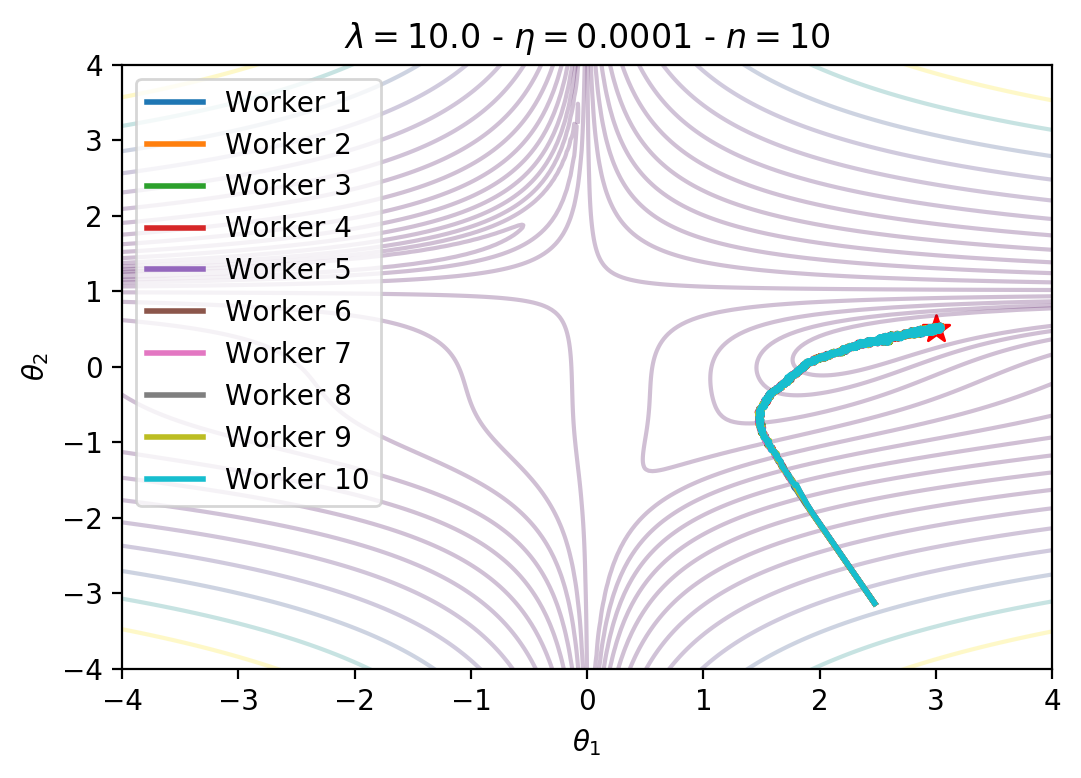
\includegraphics[width=\linewidth]{resources/images/model_averaging_identical_starting_point}
    \caption{Identical initialization}
  \end{subfigure}
  \begin{subfigure}{.49\textwidth}
    \centering
    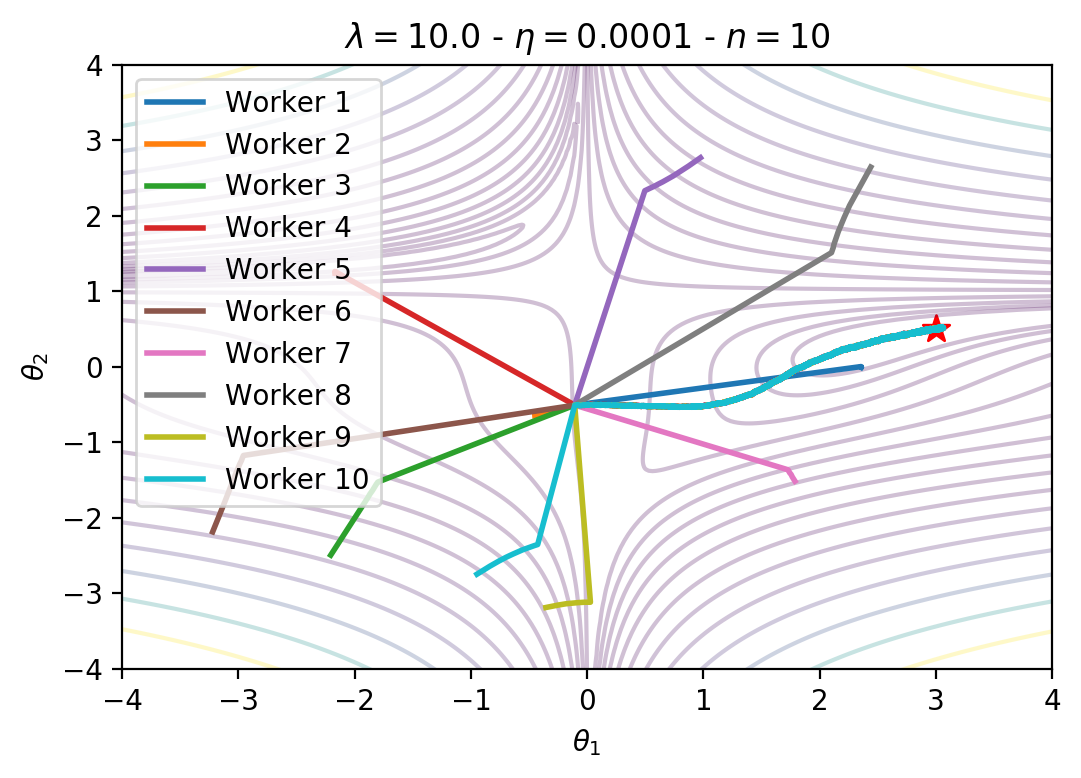
\includegraphics[width=\linewidth]{resources/images/model_averaging_cf_10}
    \caption{Random initialization}
  \end{subfigure}
  \caption{In this Figure we show the difference between identical initialization (a), and random initialization (b). In essence, both methods require roughly the same amount of time as a sequential optimization algorithm, i.e., not distributed, while using more resources. However, the difference here is that using random initialization requires a ``warmup'' period (a single parameter server update), before the actual optimization process can start. In order to simulate the stochastic noise of mini-batch gradient descent, we added a noise term to our gradient computations which was sampled from $X \sim \mathcal{N}(\mu = 0,\,\sigma^{2} = 10.0)$ to ensure that some deviation from the central variable was possible.}
  \label{fig:model_averaging_slow}
\end{figure}

\newpage

\begin{algorithm}[H]
  \caption{Describes the worker procedure with local worker exploration. The worker will be identified with a certain index $k$ and will be initialized by assigning the central variable ($\tilde{\theta}_t$) to the worker, or the worker variable can be randomized at the start of the optimization procedure. Furthermore, we introduce a hyperparameter $\lambda$, which is the number of local updates that have to be performed in order the worker parameterization $\theta^k_t$ is communicated with the parameter server.}
  \label{algo:model_averaging_worker}
  \begin{algorithmic}[1]
    \Procedure{ModelAveragingWorker}{$k$}
    \State $\theta^k_0 \gets \Call{Pull()}{}$ or $\Call{Random()}{}$ \Comment{Worker variable $\theta^k_0$ can be randomized.}
    \State $t \gets 0$
    \While{$\textbf{not}$ converged}
    \State $i \gets 0$
    \For{$i < \lambda$}
    \State $\textbf{x},~\textbf{y} \gets \Call{FetchNextMiniBatch()}{}$
    \State $\theta^k_{t + 1} \gets \theta^k_t - \eta_t \odot \nabla_\theta \mathcal{L}(\theta^k_t;\textbf{x};\textbf{y})$ \Comment{Optimization step, could be \cite{kingma2014adam}, or other optimizer.}
    \State $i \gets i + 1$
    \State $t \gets t + 1$
    \EndFor
    \State $\Call{Commit}{\theta^k_t}$
    \State $\Call{WaitForOtherWorkers()}{}$
    \State $\theta^k_t \gets \Call{Pull()}{}$
    \EndWhile
    \EndProcedure
  \end{algorithmic}
\end{algorithm}

\vspace*{1cm}

\begin{figure}[H]
  \centering
  %% 1
  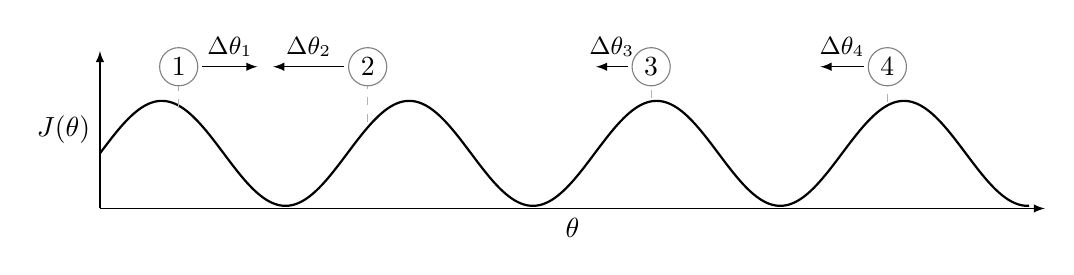
\begin{tikzpicture}
    % Draw the axis of the plots.
    \draw[->] (0,0) -- (12,0) node[midway, below] {$\theta$};
    \draw[->] (0,0) -- (0, 2) node[midway, left] {$J(\theta)$};
    % Draw the hypothesis space, which is sin(x) / 2 + 0.55
    \draw[samples=400,domain=0:11.8,smooth,variable=\x,black,thick]  plot ({\x},{sin(deg(\x * 2)) / 1.5 + 0.7});
    % Draw the instances, and their gradient arrows.
    \draw (1,1.8) node[circle,inner sep=2pt,draw=black!50] {1};
    \draw[dashed, draw=black!30] (1,1.28) -- (1,1.55);
    \draw[->] (1.3,1.8) -- (2,1.8) node[midway, above] {\small $\Delta\theta_1$};

    \draw (3.4,1.8) node[circle,inner sep=2pt,draw=black!50] {2};
    \draw[dashed, draw=black!30] (3.4,1.1) -- (3.4,1.55);
    \draw[->] (3.1,1.8) -- (2.2,1.8) node[midway, above] {\small $\Delta\theta_2$};

    \draw (7,1.8) node[circle,inner sep=2pt,draw=black!50] {3};
    \draw[dashed, draw=black!30] (7,1.4) -- (7,1.55);
    \draw[->] (6.7,1.8) -- (6.3,1.8) node[midway, above] {\small $\Delta\theta_3$};

    \draw (10,1.8) node[circle,inner sep=2pt,draw=black!50] {4};
    \draw[dashed, draw=black!30] (10,1.35) -- (10,1.55);
    \draw[->] (9.7,1.8) -- (9.15,1.8) node[midway, above] {\small $\Delta\theta_4$};
  \end{tikzpicture}
  %% 2
  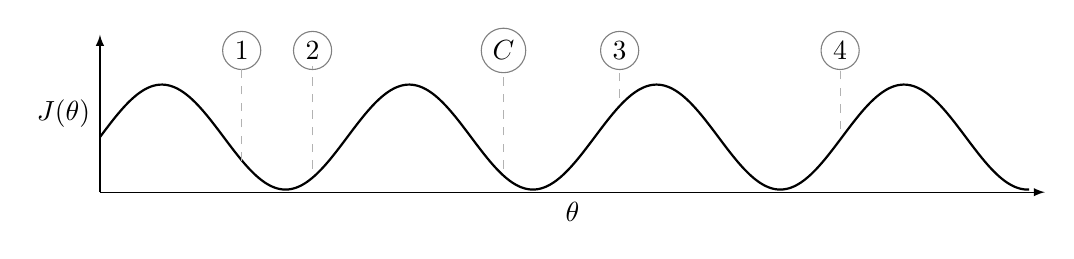
\begin{tikzpicture}
    % Draw the axis of the plots.
    \draw[->] (0,0) -- (12,0) node[midway, below] {$\theta$};
    \draw[->] (0,0) -- (0, 2) node[midway, left] {$J(\theta)$};
    % Draw the hypothesis space, which is sin(x) / 2 + 0.55
    \draw[samples=400,domain=0:11.8,smooth,variable=\x,black,thick]  plot ({\x},{sin(deg(\x * 2)) / 1.5 + 0.7});
    % Draw the instances, and their gradient arrows.
    \draw (1.8,1.8) node[circle,inner sep=2pt,draw=black!50] {1};
    \draw[dashed, draw=black!30] (1.8,0.4) -- (1.8,1.6);

    \draw (2.7,1.8) node[circle,inner sep=2pt,draw=black!50] {2};
    \draw[dashed, draw=black!30] (2.7,0.3) -- (2.7,1.6);

    \draw (6.6,1.8) node[circle,inner sep=2pt,draw=black!50] {3};
    \draw[dashed, draw=black!30] (6.6,1.2) -- (6.6,1.6);

    \draw (9.4,1.8) node[circle,inner sep=2pt,draw=black!50] {4};
    \draw[dashed, draw=black!30] (9.4,0.8) -- (9.4,1.6);
    % Draw the center variable.
    \draw (5.125,1.8) node[circle,inner sep=2pt, draw=black!50] {$C$};
    \draw[dashed, draw=black!30] (5.125,0.3) -- (5.125,1.5);
  \end{tikzpicture}
  %% 3
  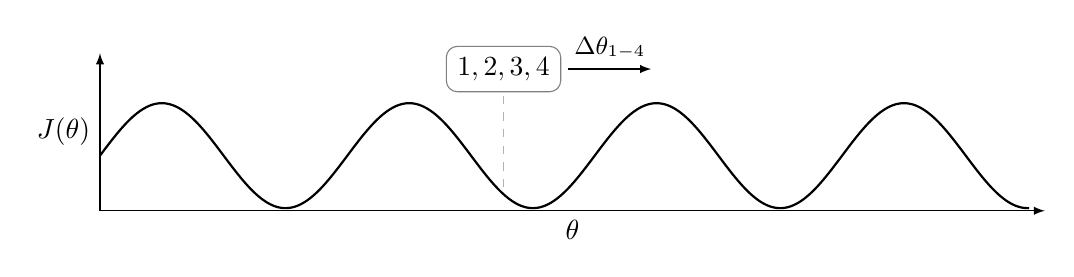
\begin{tikzpicture}
    % Draw the axis of the plots.
    \draw[->] (0,0) -- (12,0) node[midway, below] {$\theta$};
    \draw[->] (0,0) -- (0, 2) node[midway, left] {$J(\theta)$};
    % Draw the hypothesis space, which is sin(x) / 2 + 0.55
    \draw[samples=400,domain=0:11.8,smooth,variable=\x,black,thick]  plot ({\x},{sin(deg(\x * 2)) / 1.5 + 0.7});
    % Draw the instances, and their gradient arrows.
    \draw (5.125,1.8) node[rectangle,rounded corners,inner sep=4pt, draw=black!50] {$1,2,3,4$};
    \draw[dashed, draw=black!30] (5.125,0.3) -- (5.125,1.5);
    \draw[->] (5.95,1.8) -- (7,1.8) node[midway, above] {\small $\Delta\theta_{1-4}$};
  \end{tikzpicture}
  \caption{This figure explains the intuition behind model averaging. In the first state, all workers, $w_1$, $w_2$, $w_3$, and $w_4$, are uniformly initialized over the hypothesis space. Using the local parametrizations, every worker obtains an update $\Delta w_i$, and applies it locally. Afterwards, all workers send their parametrizations to the parameter server which will average them to obtain a central variable, which is depicted by $C$ in this particular figure. Finally, all workers fetch the most recent central variable, and start computing new gradients based for the following iteration.  Furthermore, what can be observed directly from this figure, is that when the workers do not agree on a \emph{local neighborhood}, the central variable will not be able to converge. This is additional support for Hypothesis~\ref{hyp:local_optimization}.}
  \label{fig:model_averaging_intuition}
\end{figure}

Nevertheless, what is interesting about the random initialization of workers, is that when we increase the number of workers, the probability that we will find a better solution (minima) compared to a sequential optimization process increases. However, this also depends on the curvature of the error space. For example, in Figure~\ref{fig:model_averaging_prob} we use Beale's function to obtain our statistic. However, from the plots we can deduce that the curvature of the error space is slightly biased towards the global minimum if first-order gradients are used. If the error space was not biased towards a specific minima, the statistic for a single worker under different hyperparameterizations should be 50\%.\\

Furthermore, what is the role of the exploration parameter $\lambda$? Does it contribute to to the optimization process besides reducing the amount of communication with the parameter server by increasing the amount of local work? In principle this would help to optimization process since more exploration of the parameter space occurs, and as a result, better updates are applied. Furthermore, remember what we said in Section~\ref{sec:ddl_introduction} on synchronous data parallelism, that effectivly increasing the number of workers implicitly increases the size of the mini-batch. Yet, in this particular case there is a subtle difference, i.e., local exploration of the parameter space. As a result, it is not implicitly increasing the size of the mini-batch since some form of local exploration occurs. As a result, \emph{the averaged central variable will produce a less-noisy consensus based on the (local) exploration of the error space}.  However, the problem lies in the fact when different sets of workers enter different minima, possibly because of \emph{too much exploration of the error space}, as depicted in Figure~\ref{fig:model_averaging_intuition}. Because if this happens, then the averaging step could potentially reset the situation instead of continuing exploring a single minima.

\begin{figure}
  \centering
  \begin{subfigure}{.35\textwidth}
    \centering
    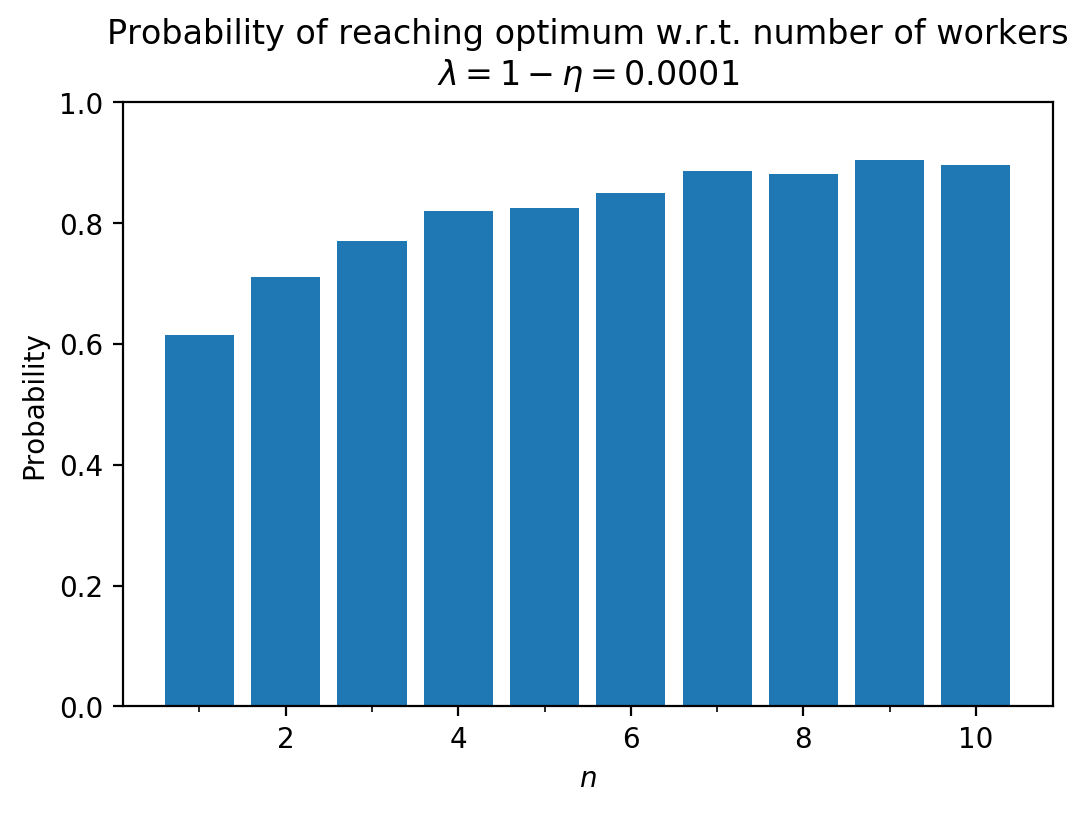
\includegraphics[width=\linewidth]{resources/images/model_averaging_prob_1}
    \caption{$\lambda = 1$}
  \end{subfigure}
  \begin{subfigure}{.35\textwidth}
    \centering
    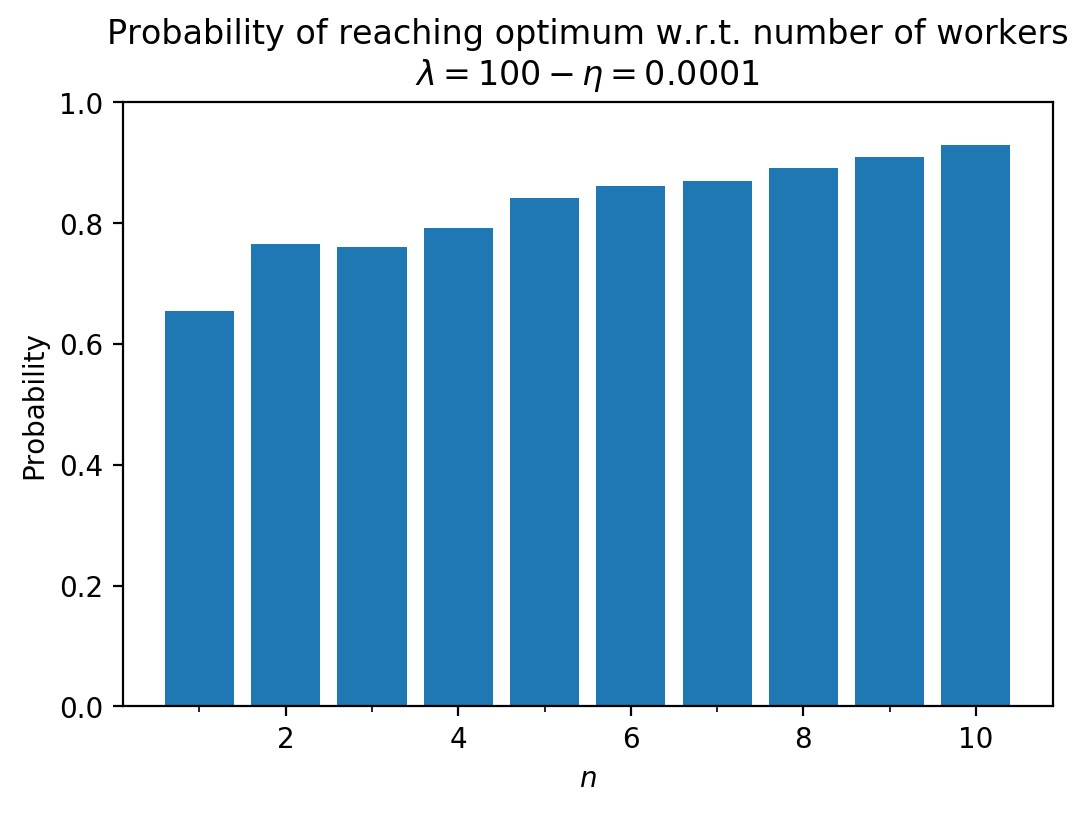
\includegraphics[width=\linewidth]{resources/images/model_averaging_cf_100_prob}
    \caption{$\lambda = 100$}
  \end{subfigure}
  \caption{Probability distribution extracted from several Monte-Carlo simulations under different conditions. We find that the probability of reaching the optimum (Beale's function) increases when the number of random initialized workers increases. Despite the fact that we observe that more exploration ($\lambda$) yiels a better statistic, we believe that this result is not significant due to the relatively low number of simulations (1000 per worker per hyperparameter).}
  \label{fig:model_averaging_prob}
\end{figure}

\begin{figure}[H]
  \centering
  \begin{subfigure}{.24\textwidth}
    \centering
    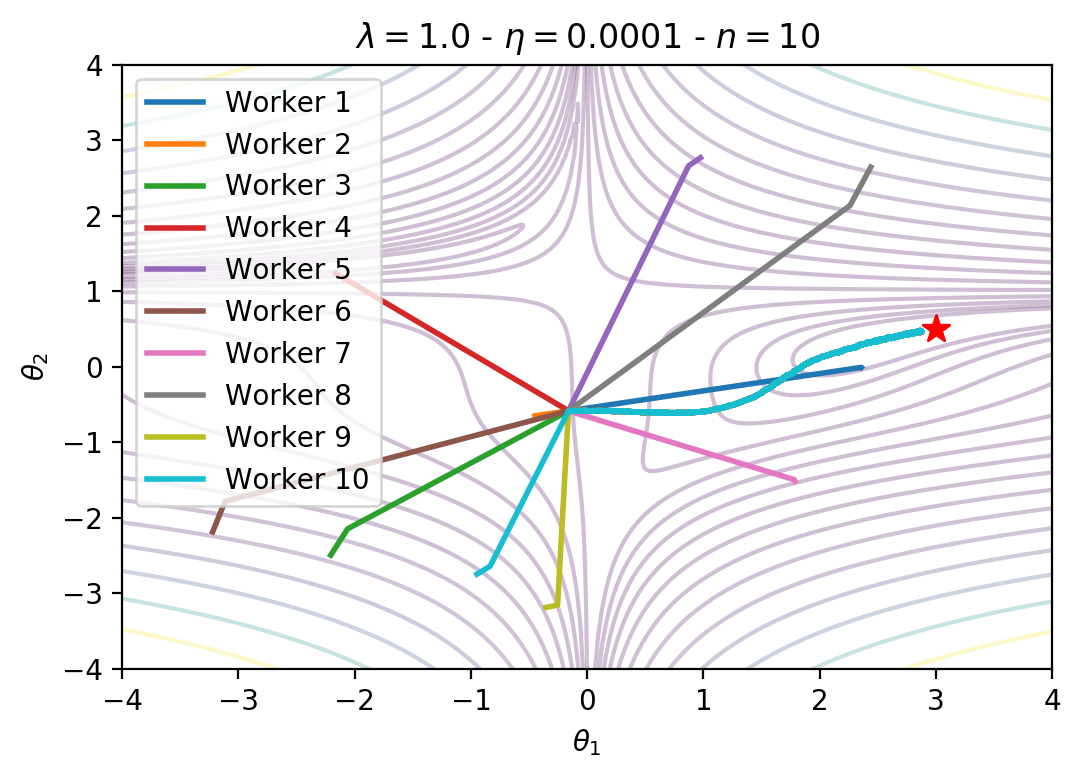
\includegraphics[width=\linewidth]{resources/images/model_averaging_cf_1}
    \caption{$\lambda = 1$}
  \end{subfigure}
  \begin{subfigure}{.24\textwidth}
    \centering
    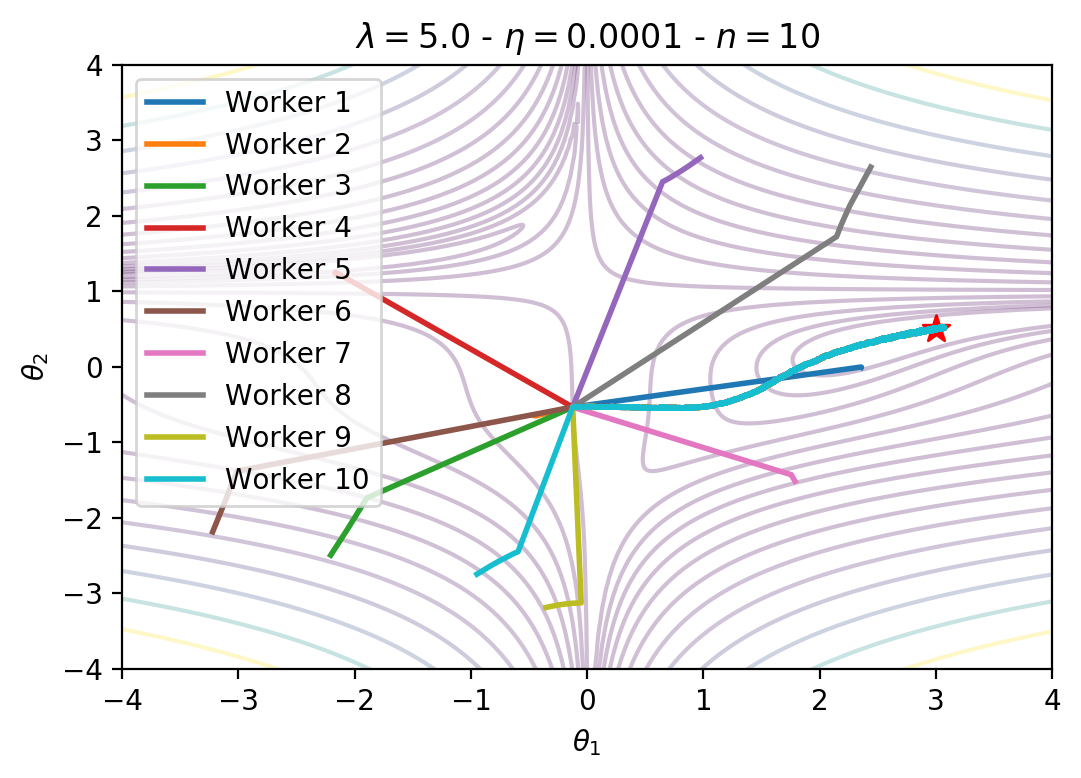
\includegraphics[width=\linewidth]{resources/images/model_averaging_cf_5}
    \caption{$\lambda = 5$}
  \end{subfigure}
  \begin{subfigure}{.24\textwidth}
    \centering
    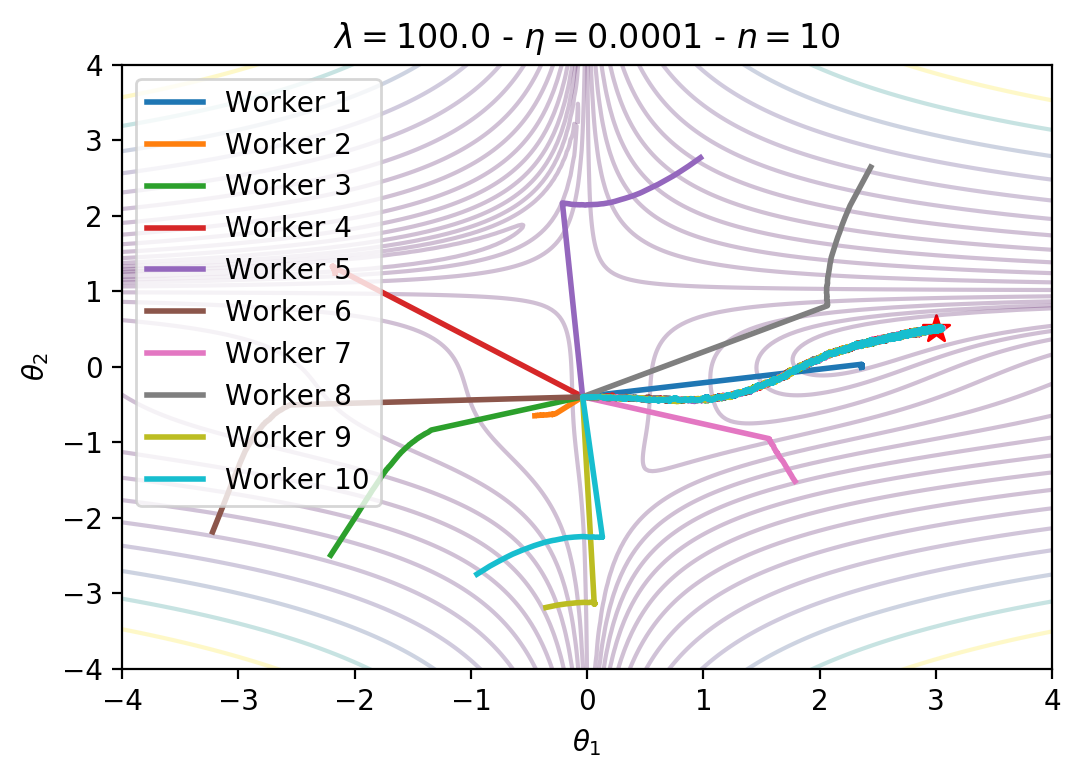
\includegraphics[width=\linewidth]{resources/images/model_averaging_cf_100}
    \caption{$\lambda = 100$}
  \end{subfigure}
  \begin{subfigure}{.24\textwidth}
    \centering
    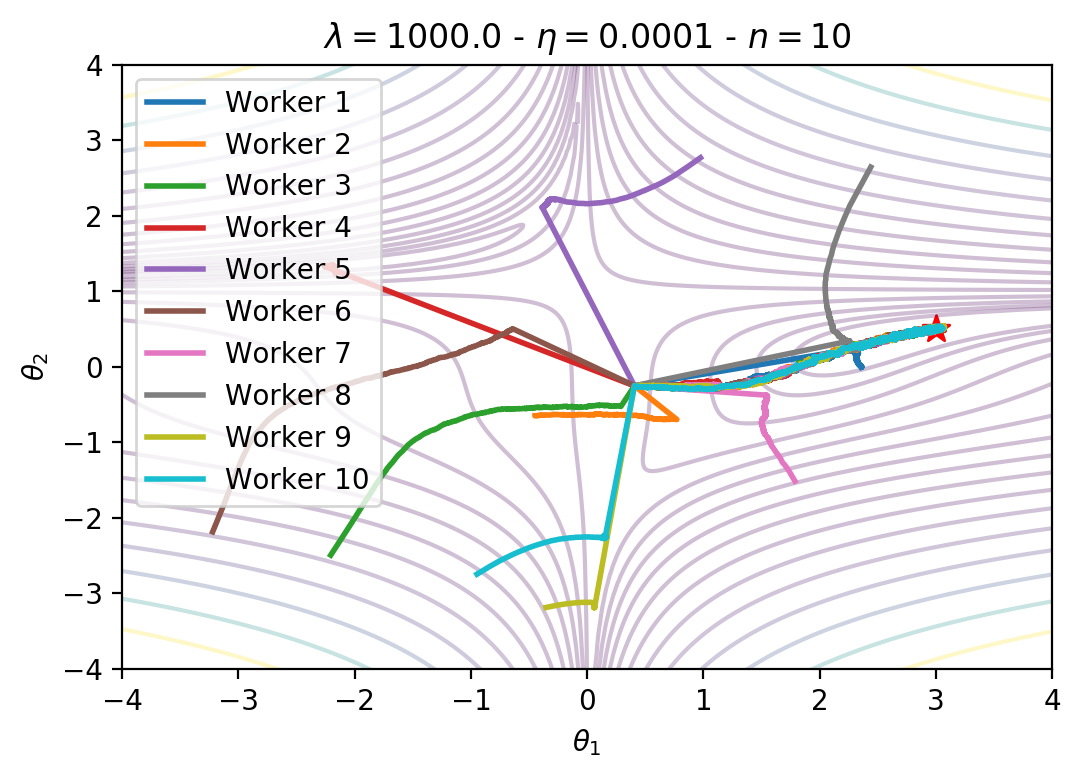
\includegraphics[width=\linewidth]{resources/images/model_averaging_cf_1000}
    \caption{$\lambda = 1000$}
  \end{subfigure}
  \label{fig:model_averaging_cf}
  \caption{Workers which have been randomly initialized (experiments use same initialization) with different values for $\lambda$ (communication frequency, or number of local worker iterations). Since the workers are initially randomized of the hypothesis space, the central variable in the first averaging step will be shifted towards the global minima because of the amount of local exploration, and due to the bias of the error space as shown in Figure~\ref{fig:model_averaging_prob}.}
\end{figure}

\subsection{Elastic Averaging SGD}
\label{sec:easgd}

Elastic Averaging SGD, or \textsc{easgd}~\cite{zhang2015deep}, is a distributed optimization algorithm designed with communication constraints in mind. In essence, \textsc{easgd} could be viewed as an extension of model averaging described in Section~\ref{sec:model_averaging} with the difference that the workers, and the central variable are coordinated using an \emph{elastic force}~\cite{zhang2015deep} instead of averaging the workers after a fixed amount of steps. This means that instead of simply transmitting the parametrization or a gradient to the parameter server, the workers commit an \emph{elastic difference} which is defined as $\eta_t \rho (\theta^k_t - \tilde{\theta}_t)$ where $\rho$ is the \emph{elasticity} hyperparameter. Intuitively, $\rho$ describes the amount of exploration that can be performed by the workers with respect to the central variable $\tilde{\theta}_t$.\\

Assuming $\lambda = 1$, the worker update and central variable update are described in Equation~\ref{eq:easgd_sync_worker}, and Equation~\ref{eq:easgd_sync_ps} respectively. What is different compared to most other optimization schemes, is that the worker update described in Equation~\ref{eq:easgd_sync_worker} has a second component, i.e., the \emph{elastic difference}. Furthermore, note that compared to other distributed optimization schemes, the workers in \textsc{easgd} do not synchronize their parameterization with the central variable as shown in Algorithm~\ref{algo:easgd_worker}, but rather update the central variable using the elastic difference, and than use the new central variable as a new reference point to compute the following elastic differences.

\begin{equation}
  \label{eq:easgd_sync_worker}
  \theta^k_{t + 1} = \theta^k_t - \eta_t \odot \nabla_\theta \mathcal{L}(\theta^k_t;\mathbf{x}^k_t;\mathbf{y}^k_t) - \eta_t\rho(\theta^k_t - \tilde{\theta}_t)
\end{equation}

\begin{equation}
  \label{eq:easgd_sync_ps}
  \tilde{\theta}_{t+1} = \tilde{\theta}_t + \eta_t \sum_{i=0}^n \rho(\theta^i_t - \tilde{\theta}_t)
\end{equation}

\begin{figure}[H]
  \centering
  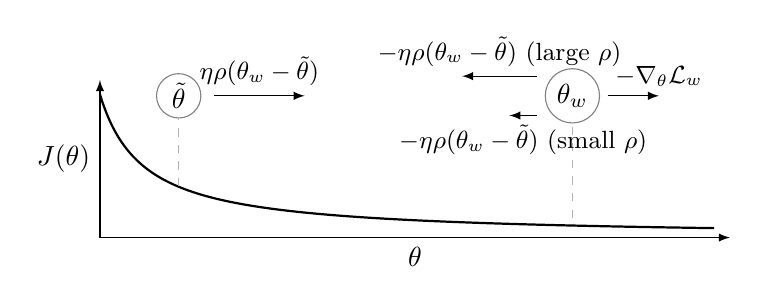
\begin{tikzpicture}
    % Draw the axis of the plots.
    \draw[->] (1,0) -- (9,0) node[midway, below] {$\theta$};
    \draw[->] (1,0) -- (1,2) node[midway, left] {$J(\theta)$};
    % Draw the function.
    \draw[samples=400,domain=1:8.8,smooth,variable=\x,black,thick]  plot ({\x},{(1 / (\x - 0.45))});
    % Draw the instances (including the center variable) with the gradient arrows and the elastic difference.
    \draw (2, 1.8) node[circle, inner sep=2pt, draw=black!50] {$\tilde{\theta}$};
    \draw[dashed, draw=black!30] (2,0.65) -- (2,1.5);
    \draw (7, 1.8) node[circle, inner sep=2pt, draw=black!50] {$\theta_w$};
    \draw[dashed, draw=black!30] (7,0.25) -- (7,1.45);
    % Draw the gradients and the elastic force.
    \draw[->] (7.45,1.8) -- (8.1,1.8) node[right, above] {\small $-\nabla_\theta \mathcal{L}_w$};
    \draw[->] (6.55,1.55) -- (6.2,1.55) node[midway, below] {\small $-\eta\rho(\theta_w - \tilde{\theta})$ (small $\rho$)};
    \draw[->] (6.55,2.05) -- (5.6,2.05) node[midway, above] {\small $-\eta\rho(\theta_w - \tilde{\theta})$ (large $\rho$)};
    % Draw elastic force applied to the central variable.
    \draw[->] (2.45, 1.8) -- (3.6, 1.8) node[midway, above] {\small $\eta\rho(\theta_w - \tilde{\theta})$};
  \end{tikzpicture}
  \caption{In this example we would like to make the intuition behind Elastic Averaging SGD clear by describing it as a classical physics problem. In this particular figure we have 1 worker, $\theta_w$ ($n = 1$, $\lambda = 1$), and a central variable $\tilde{\theta}$. The $y$-axis represents the error with respect to a certain parameterization $\theta$. Using Algorithm~\ref{algo:easgd_worker}, the worker performs $\lambda$ steps to compute the next value of $\theta_w$ using Equation~\ref{eq:easgd_sync_worker}. As stated before in Section~\ref{sec:easgd}, Equation~\ref{eq:easgd_sync_worker} holds 2 components, i.e., the regular negated first-order gradient ($-\eta_t \nabla_\theta \mathcal{L}_w$), and the \emph{negated} elastic difference ($-\eta_t\rho(\theta_w - \tilde{\theta})$). As always, the negated first-order gradient represents the steepest slope with respect to the current error (loss), and parameterization. However, the \emph{negated} elastic difference actually points towards the central variable. The magnitude of the elastic difference is controlled by hyperparameter $\rho$. This implies that a large value of $\rho$ \emph{strongly} limits the amount of exploration a worker can perform with respect to the central variable since the magnitude of the elastic difference vector will be proportionally larger compared to a small $\rho$. Finally, the central variable is updated using Equation~\ref{eq:easgd_sync_ps} and the elastic difference coming from all workers. Furthermore, we would like to note that the elastic difference during the central variable update is \emph{not} negated. Meaning that the central variable is optimized with respect to the ``pull'' of all workers, with the effect that workers whichare ahead in the optimization process, will have a larger elastic force, causing the central variable to be influenced more strongly by distant workers. Nevertheless, at the same time, distant workers are pulled towards the central variable using an equal but opposite force \emph{and} the negated gradient, i.e., the net force of the elastic difference and the negated gradient combined results either in a step towards a minimum, a null-operation, or a step in the direction of the central variable.}
  \label{fig:easgd_sync}
\end{figure}

\begin{algorithm}[H]
  \caption{Worker procedure of synchronous \textsc{easgd}. This algorithms accepts several hyperparameters, the first being the number of local computations $\lambda$, the exploration hyperparameter $\rho$, and the dynamic learning rate $\eta_t$.}
  \label{algo:easgd_worker}
  \begin{algorithmic}[1]
    \Procedure{EASGDWorker}{$k$}
    \State $\theta^k_0 \gets \tilde{\theta} \gets \Call{Pull}$
    \State $t \gets 0$
    \While{$\textbf{not}$ converged}
    \State $i \gets 0$
    \For{$i < \lambda$}
    \State $\textbf{x},~\textbf{y} \gets \Call{FetchNextMiniBatch()}{}$
    \State $\theta^k_{t + 1} \gets \theta^k_t - \eta_t \odot \nabla_\theta \mathcal{L}(\theta^k_t;\textbf{x};\textbf{y})$
    \State $i \gets i + 1$
    \State $t \gets t + 1$
    \EndFor
    \State $\mathcal{E} = \eta_t\rho(\theta^k_t - \tilde{\theta})$
    \State $\theta^k_{t+1} = \theta^k_t - \mathcal{E}$
    \State $\Call{Commit}{\mathcal{E}}$
    \State $\Call{WaitForOtherWorkers()}{}$
    \State $\tilde{\theta} \gets \Call{Pull}$
    \State $t \gets t + 1$
    \EndWhile
    \EndProcedure
  \end{algorithmic}
\end{algorithm}

However, there is an interesting property about the elastic difference which is rather problematic for the communication frequency $\lambda$. Using the intuition from Figure~\ref{fig:easgd_sync}, we can deduce that Equation~\ref{eq:easgd_sync_worker} has an additional solution for 0 besides when $\nabla_\theta \mathcal{L}(\theta^k_t;\mathbf{x}^k_t;\mathbf{y}^k_t) = 0$. This solution has profound implications on $\lambda$, and as a result, on the allocated computing resources. Because if this situation occurs, then all additional computations are wasted. Since during that time, the central variable is not updated, and the worker are not updated. In order to describe this formally, let us consider the cases for which the \textsc{easgd} worker update rule is 0, as shown in Equation~\ref{eq:easgd_sync_equilibrium_0}.

\begin{equation}
  \label{eq:easgd_sync_equilibrium_0}
  -\eta_t \odot \nabla_\theta \mathcal{L}(\theta^k_t;\mathbf{x}^k_t;\mathbf{y}^k_t) - \eta_t\rho(\theta^k_t - \tilde{\theta}_t) = 0
\end{equation}

Since we know that when a worker evaluates a 0-gradient, i.e., $\nabla_\theta \mathcal{L}(\theta^k_t;\mathbf{x}^k_t;\mathbf{y}^k_t) = 0$, then the \textsc{easgd} worker update rule is also 0. Since no change in the parameterization of the worker took place, and as a result, there is no change in the value of the elastic difference. Unless $\lambda > 1$, and in step $t - 1$, $\nabla_\theta \mathcal{L}(\theta^k_t;\mathbf{x}^k_t;\mathbf{y}^k_t) \neq 0$. In this case, a net force will be applied in the direction of the central variable, that is, the worker will move back towards the central variable.\\

Nevertheless, let us focus our efforts on the case when Equation~\ref{eq:easgd_sync_equilibrium_0} is satisfied. First, let us assume that $\nabla_\theta \mathcal{L}(\theta^k_t;\mathbf{x}^k_t;\mathbf{y}^k_t) \neq 0$. As a result, the only way that the condition described in Equation~\ref{eq:easgd_sync_equilibrium_0} can be satisfied is when the \emph{non-negated} elastic difference equals the gradient update as shown in Equation~\ref{eq:easgd_sync_equilibrium}.

\begin{equation}
  \label{eq:easgd_sync_equilibrium}
  -\eta_t \odot \nabla_\theta \mathcal{L}(\theta^k_t;\mathbf{x}^k_t;\mathbf{y}^k_t) = \eta_t\rho(\theta^k_t - \tilde{\theta}_t)
\end{equation}

Using Equation~\ref{eq:easgd_sync_equilibrium}, we can derrive a condition, described in Equation~\ref{eq:easgd_sync_working_condition}, where the amount of computational work is not wasted, and introduce an early-stopping mechanism to prevent such waste.

\begin{equation}
  \label{eq:easgd_sync_working_condition}
  \norm{-\eta_t \odot \nabla_\theta \mathcal{L}(\theta^k_t;\mathbf{x}^k_t;\mathbf{y}^k_t)} > \norm{\eta_t\rho(\theta^k_t - \tilde{\theta}_t)}
\end{equation}

One might ask why the elastic difference in Equation~\ref{eq:easgd_sync_working_condition} needs to be smaller than the gradient term in order for the worker to move towards a minima? Remember from Figure~\ref{fig:easgd_sync} that the worker only moves (backwards or forwards) whenever Equation~\ref{eq:easgd_sync_equilibrium_0} is not satisfied. As a result, we can deduce that a worker only moves towards a minima when Equation~\ref{eq:easgd_sync_working_condition} is met until the \emph{equilibrium} condition in Equation~\ref{eq:easgd_sync_equilibrium} is satisfied. At this point, a worker could stop any further local computations since additional computations would be wasted anyway. Of course, assuming the mini-batch size $m$ is sufficiently large to eradicate any noise originating from the gradients. In order to proof this result emperically, we conducted several experiments with ordinary hyperparameters ($\lambda = 30$, $\eta = 0.00001$, $n = 5$) for different values of $\rho$ summarized in Figure~\ref{fig:easgd_sync_equilibrium} and Figure~\ref{fig:easgd_sync_equilibrium_small_rho}. What we observe in both cases is that the workers initially perform a large amount of exploration due to the relatively large value of $\lambda$. Since $\lambda$ has a large value, the workers do not often synchronize with the central variable causing them to reach the equilibrium condition described in Equation~\ref{eq:easgd_sync_equilibrium} because the gradients are nog large enough to satisfy Equation~\ref{eq:easgd_sync_working_condition}.\\

To summarize, if the gradients produced by the workers are not large enough to produce a net force in the direction of a minima, then the workers are in an equilibrium with the elastic difference causing additional computational work to be wasted since the elastic difference will only lower if the distance between the worker and the central variable gets smaller. An obvious solution to this problem would be to lower the value of $\lambda$ or $\rho$. However, lowering the value of $\lambda$ causes the worker to communicate more frequently with the parameter server, even if the equilibrium condition is not met. Since \textsc{easgd} is designed with communication constraints in mind, this is not an ideal solution. Furthermore, lowering $\rho$ is also not ideal since this would reduce the equilibrium condition even further, causing workers to deviate further from the central variable. As mentioned before in Section~\ref{sec:model_averaging} this is not desired because the possibility exists that different sets of workers will fall into different minima. This is especially problematic in \textsc{easgd} since the parameterizations of the workers are not synchronized with the central variable, but are coordinated using the elastic difference. For example, imagine the case when two sets of workers (equal in number) are in two different minima with the central variable being in the middle of these two sets. Furthermore, assume that the elastic difference in these two sets of workers is identical and Equation~\ref{eq:easgd_sync_equilibrium} is satisfied. This implies that the central variable and the workers are not able to move, even after a synchronization step, which in turn results in the fact that the central variable is not able to converge.

\begin{figure}[H]
  \centering
  \begin{subfigure}{.45\textwidth}
    \centering
    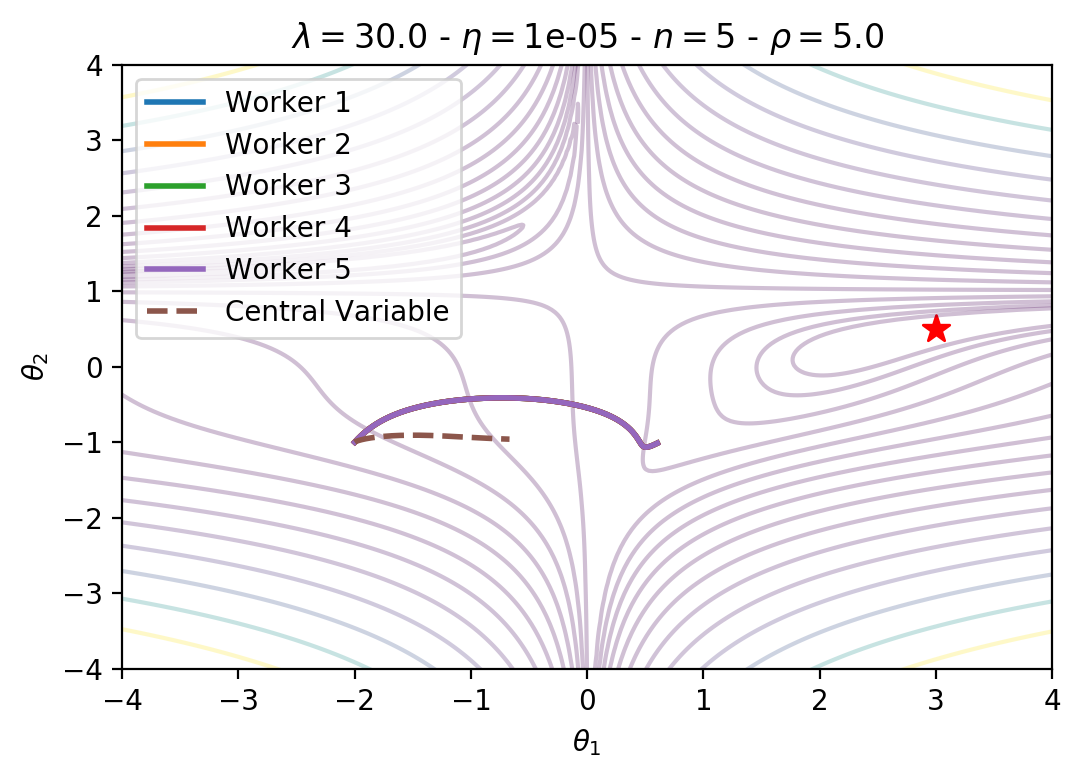
\includegraphics[width=\linewidth]{resources/images/easgd_sync_norm_space.png}
  \end{subfigure}
  \begin{subfigure}{.45\textwidth}
    \centering
    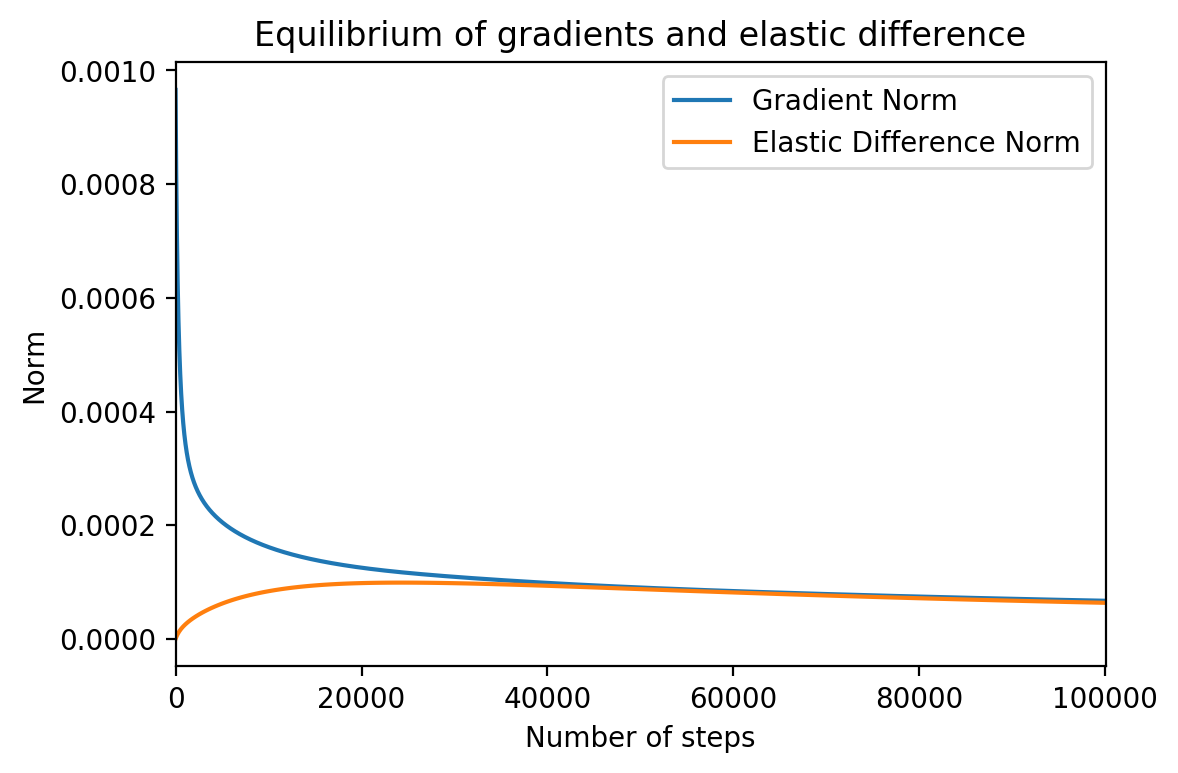
\includegraphics[width=\linewidth]{resources/images/easgd_sync_norm_equilibrium.png}
  \end{subfigure}
  \caption{In this experiment we use $\rho = 5$, as suggested by the authors~\cite{zhang2015deep}. We observe that at some point the elastic difference is starting to the influence the first-order gradients causing the workers to bend downwards, which is not present in Figure~\ref{fig:easgd_sync_equilibrium_small_rho}. This ``bend'' is due to a significant elastic force pointing in the direction of the central variable. If we would decompose the vector in its main components, i.e., $\theta_1$ and $\theta_2$, we would find that the $\theta_2$ component is significant enough to cause to worker to bend downwards since the elastic force is getting stronger proportional to the distance between the worker and the central variable and hyperparameter $\rho$. Furthermore, the equilibrium plot shows that the worker does a lot of initial exploration, while the central variable slowly follows the workers based on the averaged elastic difference. After 40000 steps, we see that the workers reach the equilibrium condition. As a result, any computational work done by the workers within a communication window is wasted since the distance between the workers and the central variable needs to grow smaller for the elastic force to shrink. However, because the elastic force is shrinking proportionally to the distance between the workers and the central variable, it allows the workers to explore \emph{slightly} more of the hypothesis space since the workers already met the equilibrium condition.}
  \label{fig:easgd_sync_equilibrium}
\end{figure}

\begin{figure}[H]
  \centering
  \begin{subfigure}{.45\textwidth}
    \centering
    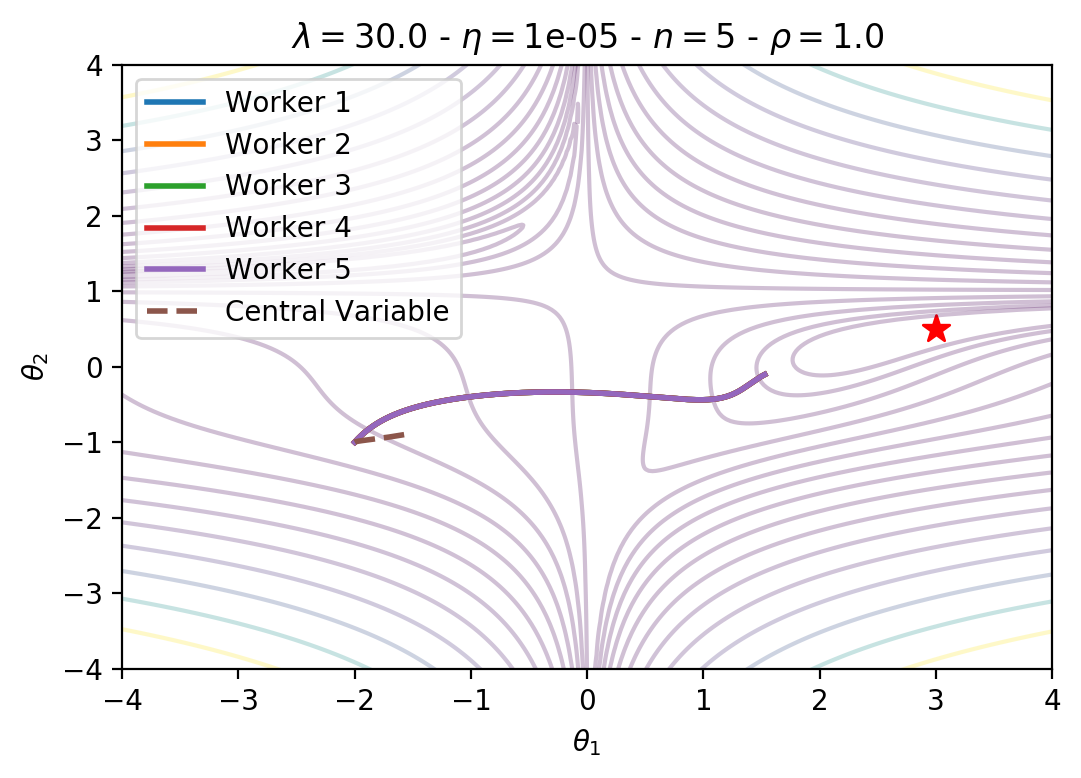
\includegraphics[width=\linewidth]{resources/images/easgd_sync_norm_space_2.png}
  \end{subfigure}
  \begin{subfigure}{.45\textwidth}
    \centering
    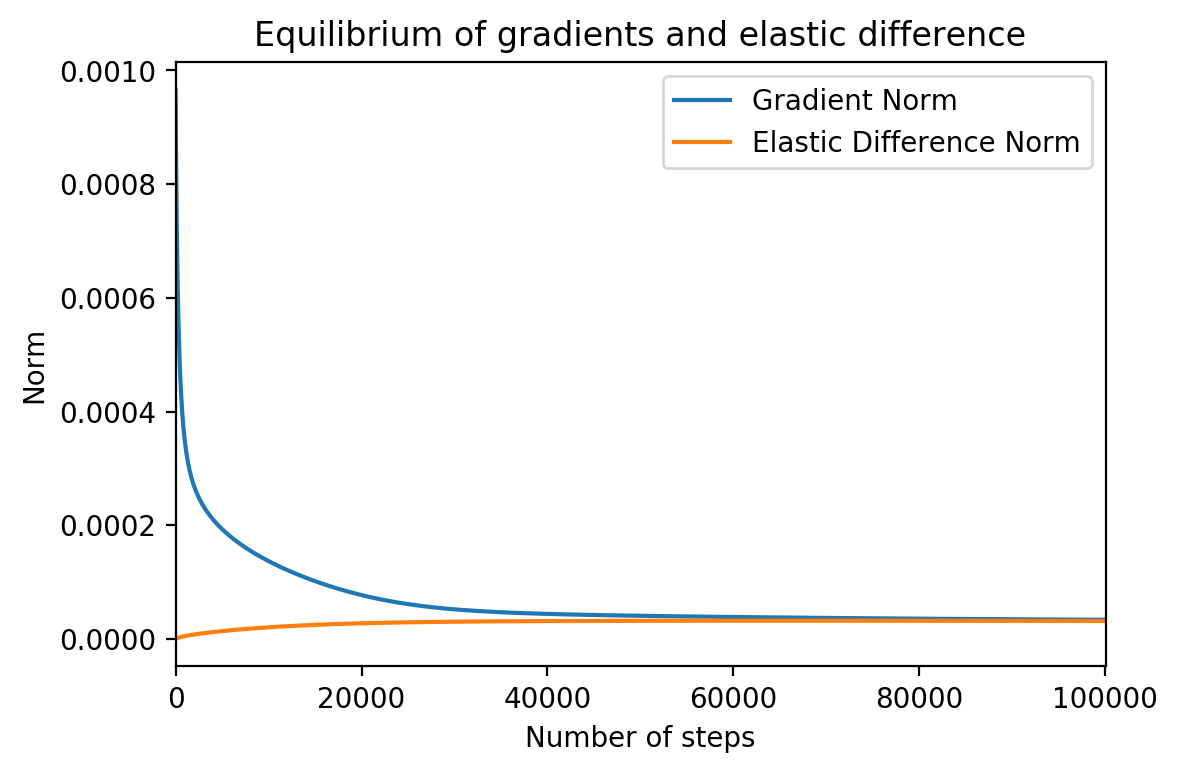
\includegraphics[width=\linewidth]{resources/images/easgd_sync_norm_equilibrium_2.png}
  \end{subfigure}
  \caption{In this experiment we reduce the value of the exploration hyperparameter $\rho$ while all other hyperparameters from our experiment in Figure~\ref{fig:easgd_sync_equilibrium} remain the same. After running the experiment we do not observe the ``bend'' which we initially observed in Figure~\ref{fig:easgd_sync_equilibrium}. However, this was expected since the elastic force is not that prominent due to the reduced value of hyperparameter $\rho$. Nevertheless, we still observe that the workers reach the equilibrium condition, with the difference that the central variable shows slower convergence behavior compared to Figure~\ref{fig:easgd_sync_equilibrium}.}
  \label{fig:easgd_sync_equilibrium_small_rho}
\end{figure}

To improve convergence of the central variable in \textsc{easgd}, and reduce the amount of wasted computational resources, we implemented Equation~\ref{eq:easgd_equilibrium_stopping_condition} based on Equation~\ref{eq:easgd_sync_working_condition} as a measure to stop wasting further computations.

\begin{equation}
  \label{eq:easgd_equilibrium_stopping_condition}
  \norm{-\eta_t \odot \nabla_\theta \mathcal{L}(\theta^k_t;\mathbf{x}^k_t;\mathbf{y}^k_t)} \leq \norm{\eta_t\rho(\theta^k_t - \tilde{\theta}_t)}
\end{equation}

However, we observed from our experiments that this exact condition is rarely satisfied. Of course, we made the assumption in Equation~\ref{eq:easgd_sync_equilibrium} that the parameterization of a worker does \emph{not} change if a worker settles in an equilibrium. Of course, before reaching the equilibrium, the gradient is non-zero, this implies that there is a change in the parameterization of a worker causing the elastic difference to be modified. With the result that the net force applied to the worker is \emph{approaching} the equilibrium. As a result, the net force applied to a worker is gradually becoming smaller.\\

In order to anticipate for a declining net force, and as a result, the gradually approaching equilibrium, we communicate the elastic difference with the parameter server if Equation~\ref{eq:easgd_equilibrium_fix} is met.

\begin{equation}
  \label{eq:easgd_equilibrium_fix}
  \Bigg(\norm{-\eta_t \odot \nabla_\theta \mathcal{L}(\theta^k_t;\mathbf{x}^k_t;\mathbf{y}^k_t)} - \norm{\eta_t\rho(\theta^k_t - \tilde{\theta}_t)}\Bigg) < \eta_t
\end{equation}

Using the same experimental configuration as in Figure~\ref{fig:easgd_sync_equilibrium}, with the difference that Equation~\ref{eq:easgd_equilibrium_fix} has been implemented as an early-stopping mechanism to communicate the elastic difference with the parameter server. Using Equation~\ref{eq:easgd_equilibrium_fix}, we can see that the proposed early stopping mechanism benefits the central variable in terms of convergence with respect to the default experimental configuration in Figure~\ref{fig:easgd_sync_equilibrium}.\\

What is remarkable about the equilibrium plot in Figure~\ref{fig:easgd_sync_fix} is the precense of a sudden drop in the norm of the elastic difference vector which is abscent in Figure~\ref{fig:easgd_sync_equilibrium} despite the fact that the workers follow similar paths. This is due to the early stopping mechanism which pulling the central variable closer towards the workers causing the decline in the norm of the elastic difference. Furthermore, since at this point the gradients are relatively small, a lot of local work can be done while at the same time the central variable will be able to keep the elastic distance small.

\begin{figure}[H]
  \centering
  \begin{subfigure}{.45\textwidth}
    \centering
    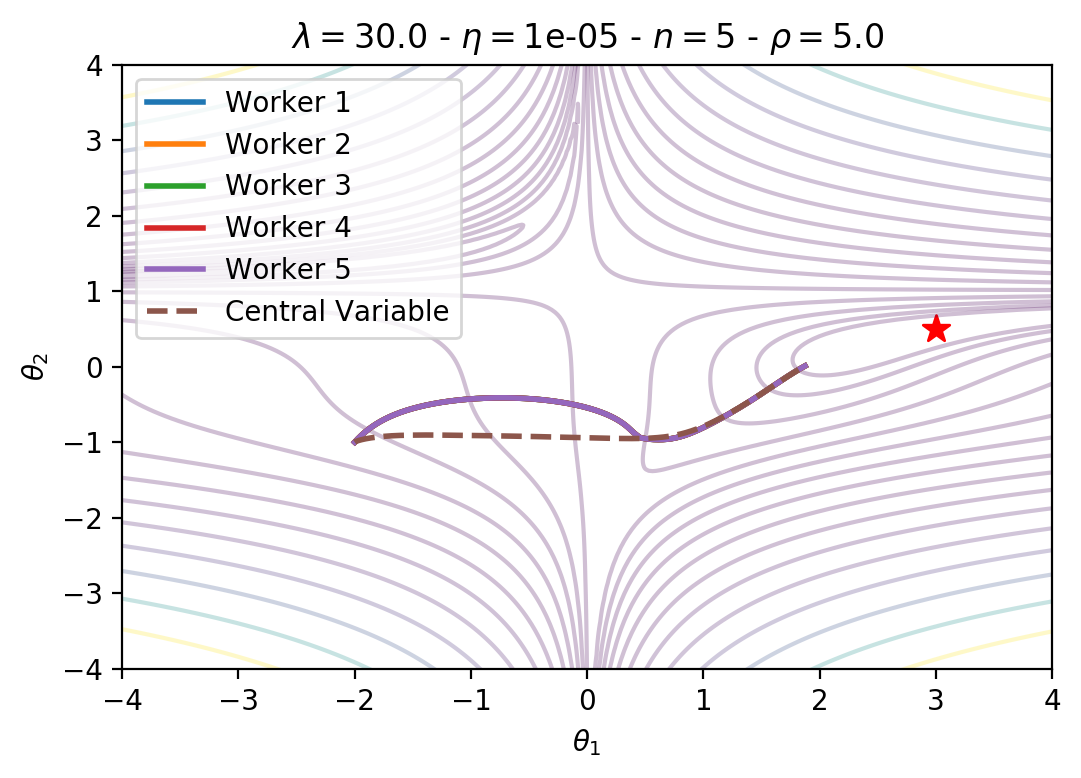
\includegraphics[width=\linewidth]{resources/images/easgd_sync_norm_space_fix.png}
  \end{subfigure}
  \begin{subfigure}{.45\textwidth}
    \centering
    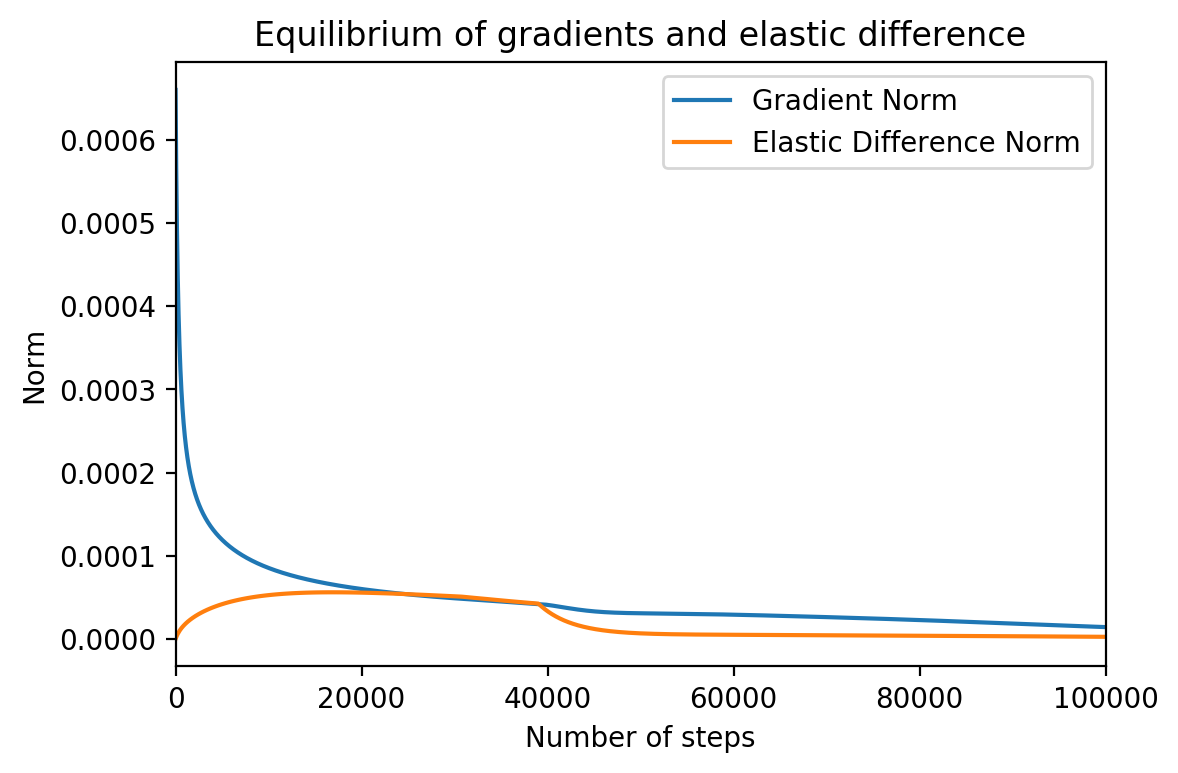
\includegraphics[width=\linewidth]{resources/images/easgd_sync_norm_ed_fix.png}
  \end{subfigure}
  \caption{\textsc{easgd} using the early stopping mechanism described in Equation~\ref{eq:easgd_equilibrium_fix}. Compared to Figure~\ref{fig:easgd_sync_equilibrium}, which uses the same experimental configuration, we observe that the central variable benefits in terms of convergence from increased communication when the early stopping condition is met.}
  \label{fig:easgd_sync_fix}
\end{figure}

Since the early stopping condition effectively communicates the elastic difference with the parameter server, is it not in essence increasing the communication frequency, i.e., lowering $\lambda$? In effect it isn't, since communication only takes place when the workers and the central variable approach an equilibrium condition. To show this, we conducted several experiments with and without the early stopping mechanism shown in Figure~\ref{fig:easgd_sync_lambda_10} and Figure~\ref{fig:easgd_sync_lambda_50}.

\begin{figure}[H]
  \centering
  \begin{subfigure}{.45\textwidth}
    \centering
    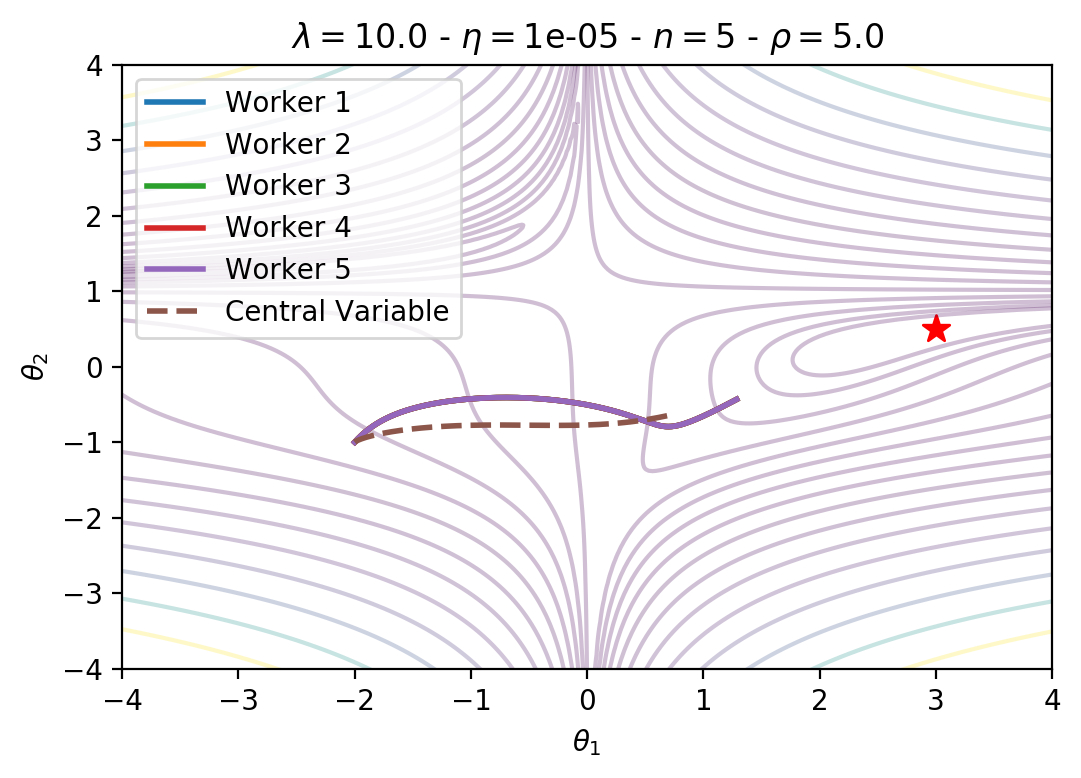
\includegraphics[width=\linewidth]{resources/images/easgd_es_10_n}
    \caption{No early stopping}
  \end{subfigure}
  \begin{subfigure}{.45\textwidth}
    \centering
    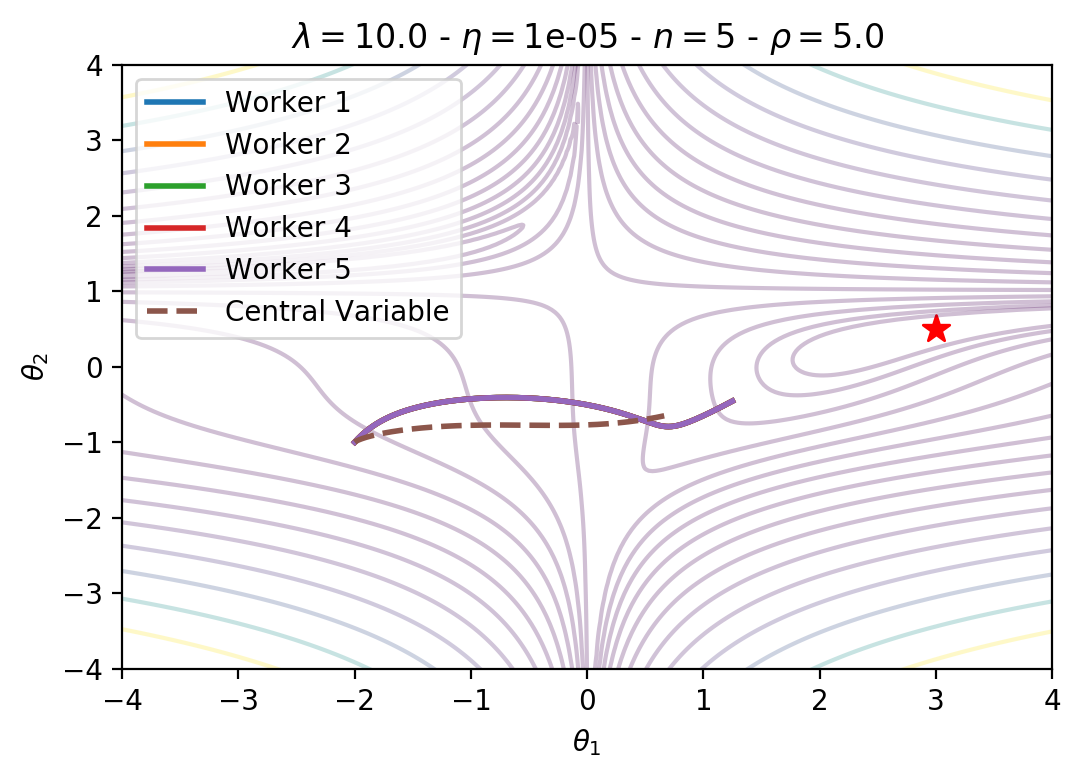
\includegraphics[width=\linewidth]{resources/images/easgd_es_10_y}
    \caption{Early stopping}
  \end{subfigure}
  \begin{subfigure}{.45\textwidth}
    \centering
    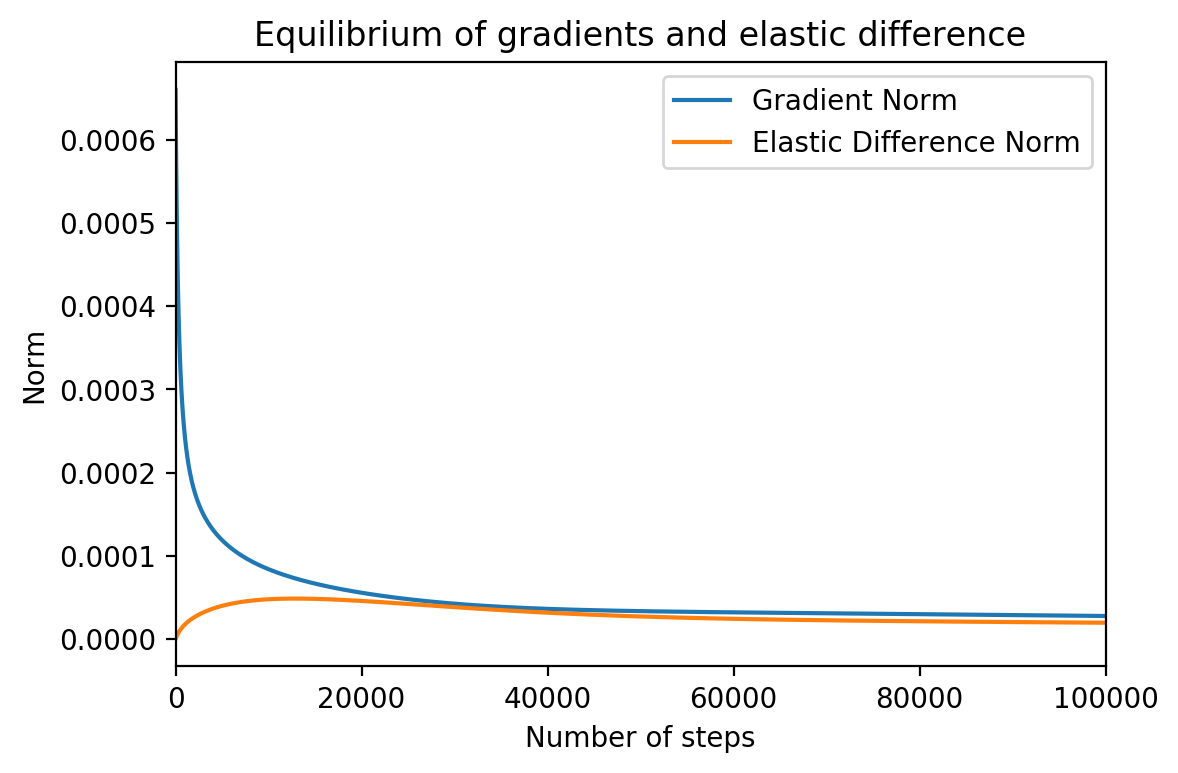
\includegraphics[width=\linewidth]{resources/images/easgd_es_10_n_eq}
    \caption{Equilibrium condition is not met (lines do not meet). As a result, early stopping is not applied.}
  \end{subfigure}
  \caption{$\lambda = 10$}
  \label{fig:easgd_sync_lambda_10}
\end{figure}

\begin{figure}[H]
  \centering
  \begin{subfigure}{.45\textwidth}
    \centering
    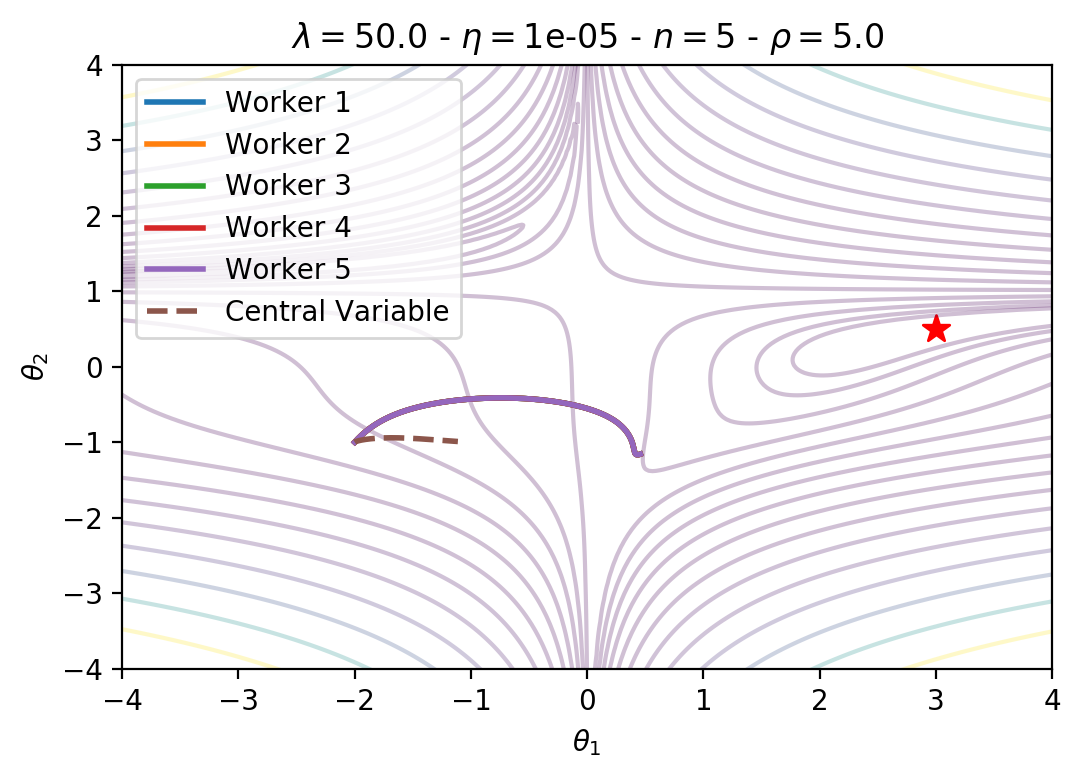
\includegraphics[width=\linewidth]{resources/images/easgd_es_50_n}
    \caption{No early stopping}
  \end{subfigure}
  \begin{subfigure}{.45\textwidth}
    \centering
    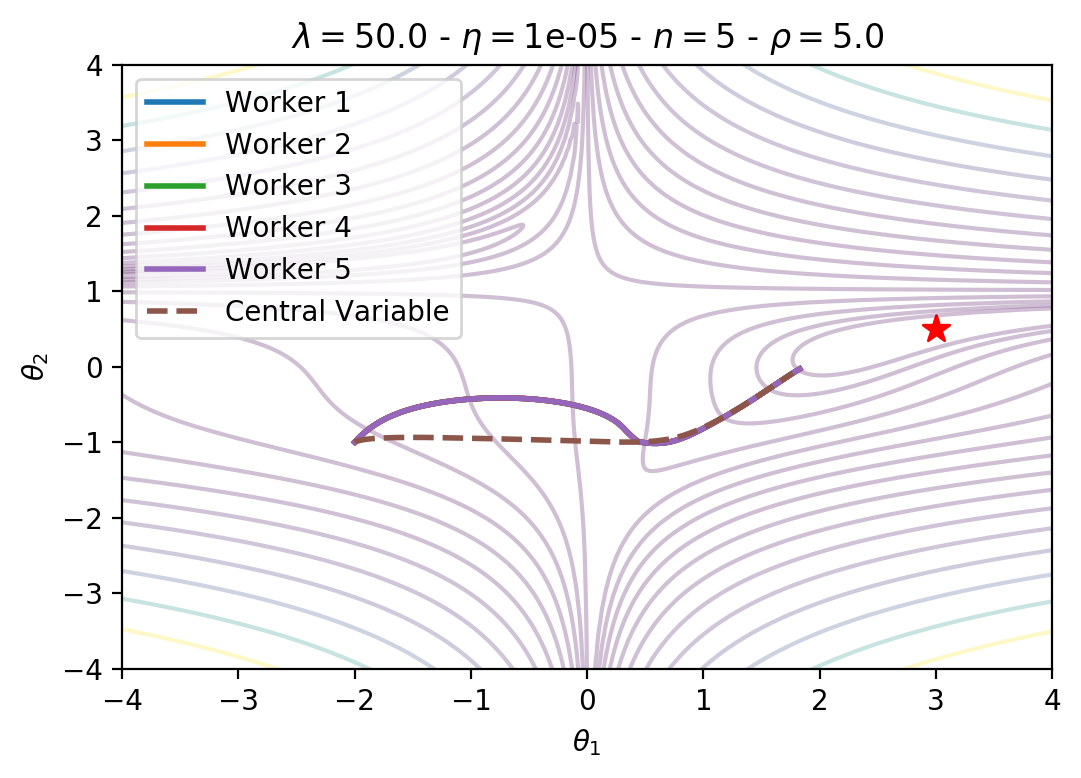
\includegraphics[width=\linewidth]{resources/images/easgd_es_50_y}
    \caption{Early stopping}
  \end{subfigure}
  \begin{subfigure}{.45\textwidth}
    \centering
    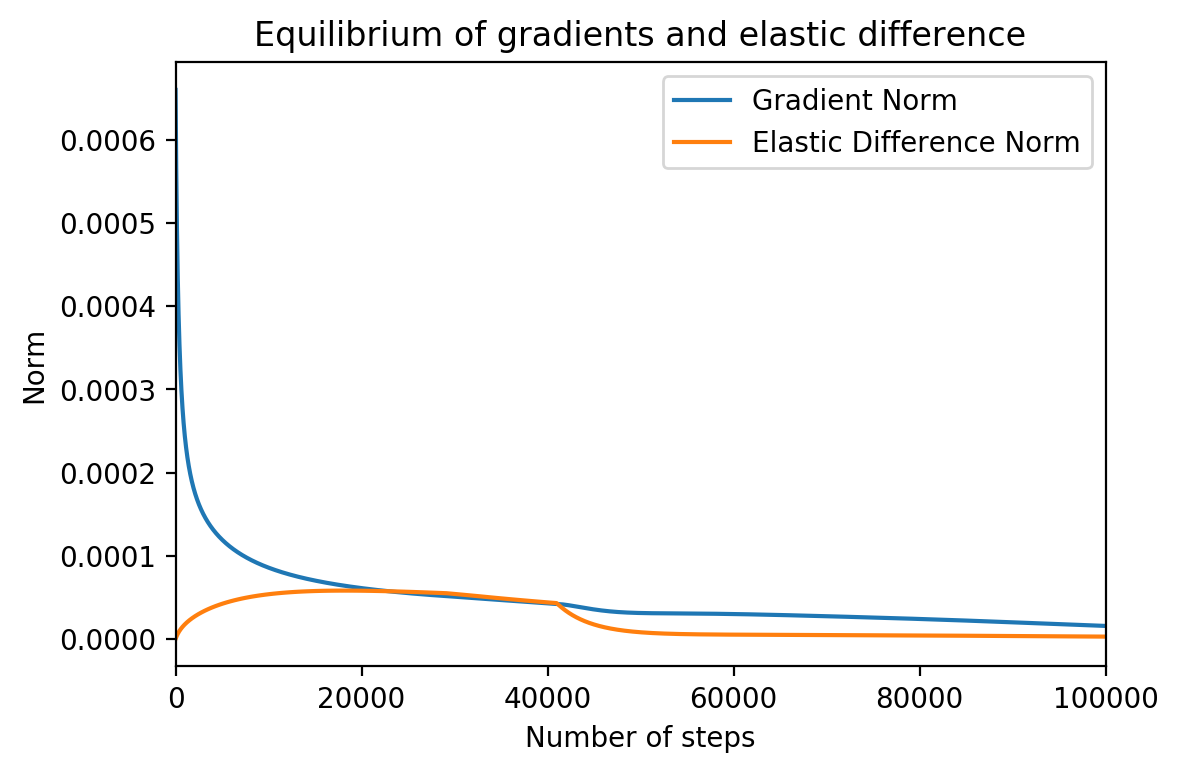
\includegraphics[width=\linewidth]{resources/images/easgd_es_50_y_eq}
    \caption{Equilibrium condition is met. Early stopping is applied.}
  \end{subfigure}
  \caption{$\lambda = 50$}
  \label{fig:easgd_sync_lambda_50}
\end{figure}

An other interesting phenomena is when \textsc{easgd} is approaching a minima. Compared to other synchronous optimizers such as mini-batch parallelism, or model averaging, \textsc{easgd} requires a significant amount of additional steps to actually converge to the minima because of the equilibrium condition as shown in Figure~\ref{fig:easgd_sync_slow}. Remember, if the workers are approaching the equilibrium condition, a small net force is applied to the worker because the \emph{negated} elastic difference counter-acts the advances of the workers to minimize the variance of the workers with respect to the central variable.

\begin{figure}[H]
  \centering
  \begin{subfigure}{.45\textwidth}
    \centering
    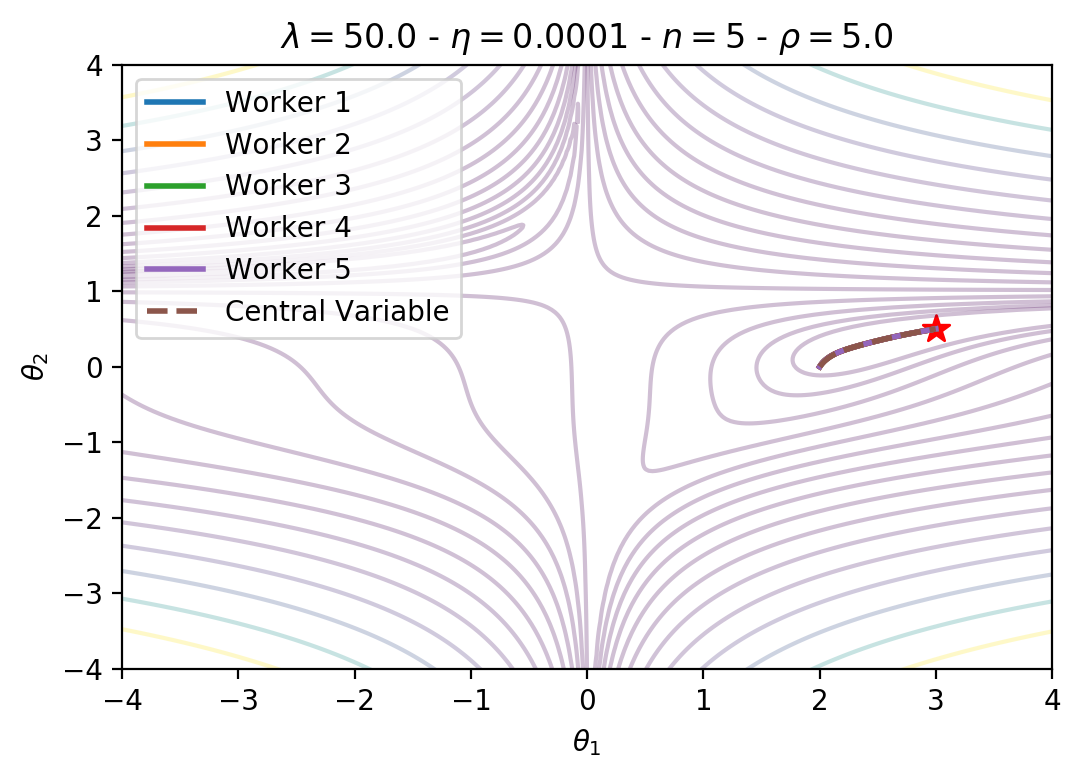
\includegraphics[width=\linewidth]{resources/images/easgd_sync_slow_space}
  \end{subfigure}
  \begin{subfigure}{.45\textwidth}
    \centering
    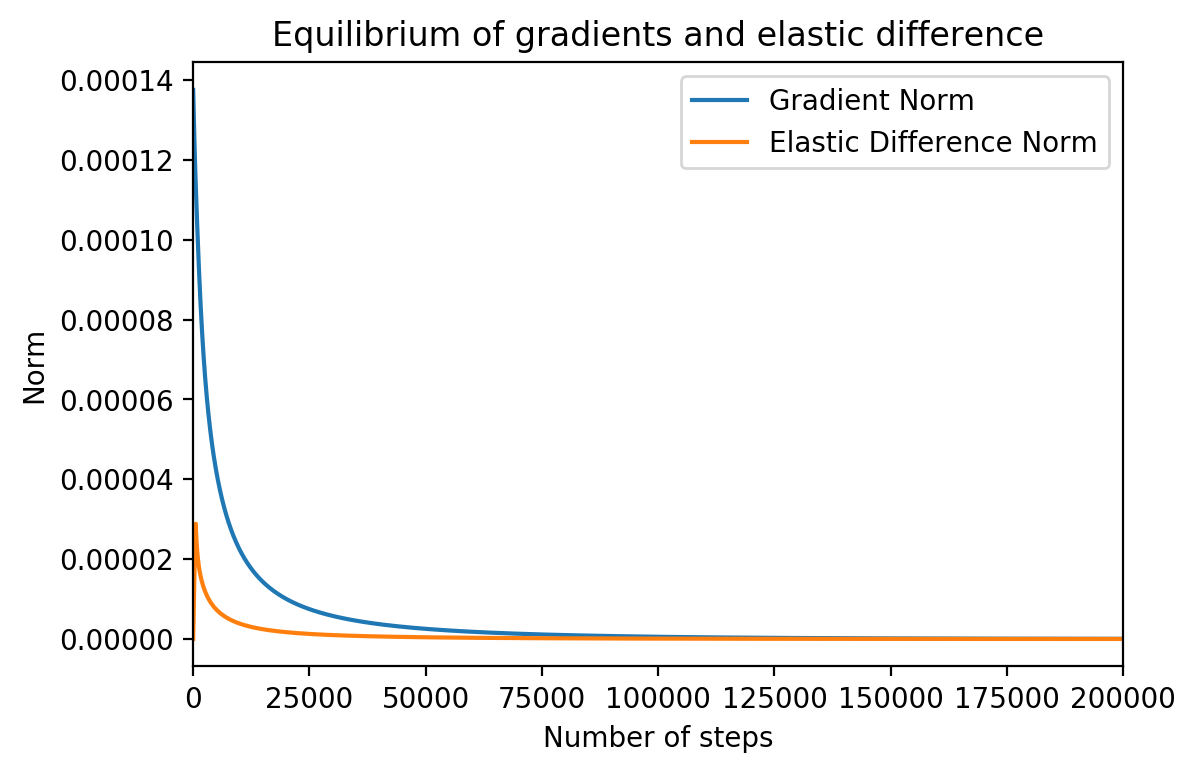
\includegraphics[width=\linewidth]{resources/images/easgd_sync_slow_eq}
  \end{subfigure}
  \caption{Slow converge of \textsc{easgd} at minima due to the equilibrium condition. In this figure we apply early stopping but due to the small gradients close to the minima it does not have any significant effects.}
  \label{fig:easgd_sync_slow}
\end{figure}

\section{Asynchronous Data Parallelism}
\label{sec:asynchronous_data_parallelism}

\subsection{DOWNPOUR}
\label{sec:downpour}

Waits induced by blocking mechanisms in synchronous data parallelism significantly reduce the harware utilisation during training, especially in non-homogeneous hardware configurations. As mentioned in Section~\ref{sec:ddl_introduction}, this can be resolved by simply removing the synchronizations barriers, as suggested by~\cite{dean2012large}. The algorithm the authors proposed is called \textsc{downpour}, and is shown in Algorithm~\ref{algo:downpour_worker}.\\

\textsc{downpour} is an intuitively a very simple algorithm. As before, we have $n$ different workers optimizing a central variable $\tilde{\theta}_t$ with the difference that every worker will \emph{commit} a gradient after every mini-batch in an asynchronous fashion, and after a commit has been performed, the worker will synchronize with the parameter server by \emph{pulling} the most recent parameterization of the central variable.

\begin{equation}
  \label{eq:downpour_worker}
  \theta^k_{t+1} = \theta^k_t - \eta_t \odot \nabla_\theta \mathcal{L}(\theta^k_t;\mathbf{x}^k_t;\mathbf{y}^k)
\end{equation}

\begin{equation}
  \label{eq:downpour_ps}
  \tilde{\theta}_{t+1} = \tilde{\theta}_t - \eta_t \odot \nabla_\theta \mathcal{L}(\theta^k_t;\mathbf{x}^k_t;\mathbf{y}^k)
\end{equation}

As mentioned in Chapter~\ref{chapter:introduction}, due to the asynchronous optimization one does not have the issue with idle workers due to synchronizations mechanisms. Instead, there is a more severe problem related to the parameterizations of the workers. Since workers will commit gradients to the central variable in an asynchronous manner, other workers will commit gradients based on older parameterizations of the central variable. As a result, the gradients of these workers are \emph{stale} as shown in Figure~\ref{fig:intro_asyn_data_parallelism} and Figure~\ref{fig:downpour_convergence}. An additional, but related issue to parameter staleness, is that increasing the amount of asynchronous workers, increases the staleness in the system as shown in Figure~\ref{fig:staleness_distribution}.

\begin{algorithm}[H]
  \caption{Worker procedure of \textsc{downpour}, which is a parallelized extension of \textsc{sgd}.}
  \label{algo:downpour_worker}
  \begin{algorithmic}[1]
    \Procedure{DOWNPOURWorker}{$k$}
    \State $\theta^k_0 \gets \tilde{\theta} \gets \Call{Pull}$
    \State $t \gets 0$
    \While{$\textbf{not}$ converged}
    \State $\textbf{x},~\textbf{y} \gets \Call{FetchNextMiniBatch()}{}$
    \State $g \gets -\eta_t \odot \nabla_\theta \mathcal{L}(\theta^k_t;\textbf{x};\textbf{y})$
    \State $\Call{Commit}{g}$
    \State $\theta^k_{t + 1} \gets \Call{Pull}$
    \State $t \gets t + 1$
    \EndWhile
    \EndProcedure
  \end{algorithmic}
\end{algorithm}

Nevertheless, contrary to \textsc{easgd}, \textsc{downpour} is not designed with communication constraints in mind. As a result, increasing the number of workers in an already saturated environment will not reduce the training time since whenever a worker computes a gradient, it will commit the result to the parameter server. To illustrate this, imagine having several workers committing highly dimensional gradients to the parameter server. Since it takes some time to incorperate these gradients into the central variable, other workers will have to wait for their turn in the queue. To reduce the side-effects (waits) in this particular situation,~\cite{louppe2010zealous} proposes to before committing the gradient, a worker should send a small control message to check if the queue is currently occupied, i.e., gradients of other workers are being incorperated into the central variable. If this is the case, do not commit the gradient, but fetch the next mini-batch, compute the gradient, and accumulate the computed gradient with the previously computed gradient, and send a new control message\\

An obvious problem with this method is that the possibility exists that after $x$ number of retries, the central variable queue is still occupied by other workers. Following the naive procedure, the zealous method should keep accumulating new gradients. However, this is problematic at step $x + 1$, when the queue is available. Imagine the possibility that other workers, and the central variable converged to a different minima. If our worker would commit the accumulated gradient in this particular situation, then the central variable would not be close to its minima as it was before. In order to reduce the amount of staleness in such a situation, one could introduce a limit to the amount of local steps that can be made in an attempt to reduce staleness as shown in Algorithm~\ref{algo:downpour_worker_zealous}.\\

However, this technique introduces an additional hyperparameter. Several other approaches which handle this problem in a different way without introducing new hyperparameters, and additionally giving some intuition and insight into parameter staleness in Deep Learning are discussed in detail in Chapter~\ref{chapter:accumulated_gradient_normalization} and Chapter~\ref{chapter:asynchronous_distributed_adaptive_gradients}.

\begin{algorithm}[H]
  \caption{Zealous worker procedure of \textsc{downpour}, inspired by~\cite{louppe2010zealous}.}
  \label{algo:downpour_worker_zealous}
  \begin{algorithmic}[1]
    \Procedure{ZealousDOWNPOURWorker}{$k$}
    \State $\theta^k_0 \gets \tilde{\theta} \gets \Call{Pull}$
    \State $t \gets 0$
    \While{$\textbf{not}$ converged}
    \State $i \gets 0$
    \State $g \gets 0$
    \While{$i < \lambda$}
    \State $\textbf{x},~\textbf{y} \gets \Call{FetchNextMiniBatch()}{}$
    \State $g \gets g -\eta_t \odot \nabla_\theta \mathcal{L}(\theta^k_t;\textbf{x};\textbf{y})$
    \If{$\textbf{not}$~\Call{QueueOccupied}~}
    \State $\Call{Commit}{g}$
    \State $\theta^k_{t + 1} \gets \Call{Pull}$
    \EndIf
    \State $t \gets t + 1$
    \State $i \gets i + 1$
    \EndWhile
    \EndWhile
    \EndProcedure
  \end{algorithmic}
\end{algorithm}

\begin{figure}[H]
  \centering
  \begin{subfigure}{.49\textwidth}
    \centering
    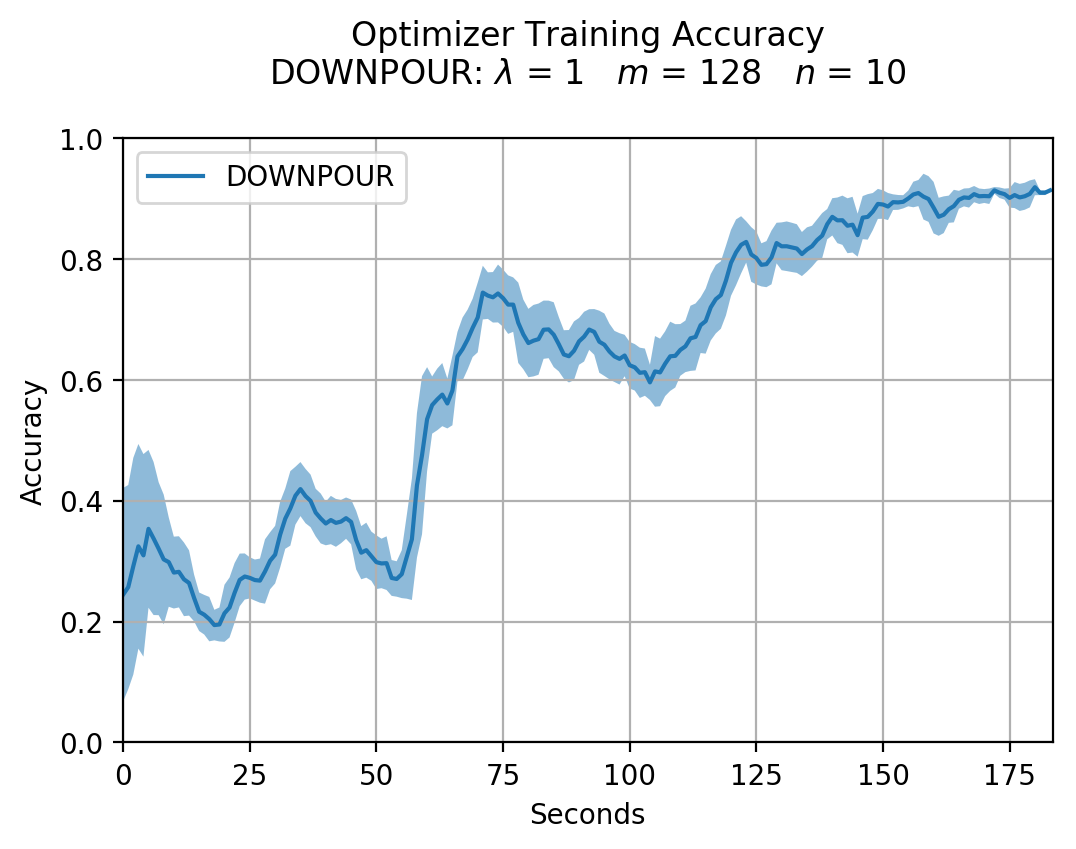
\includegraphics[width=\linewidth]{resources/images/downpour_10}
    \caption{$n = 10$}
  \end{subfigure}
  \begin{subfigure}{.49\textwidth}
    \centering
    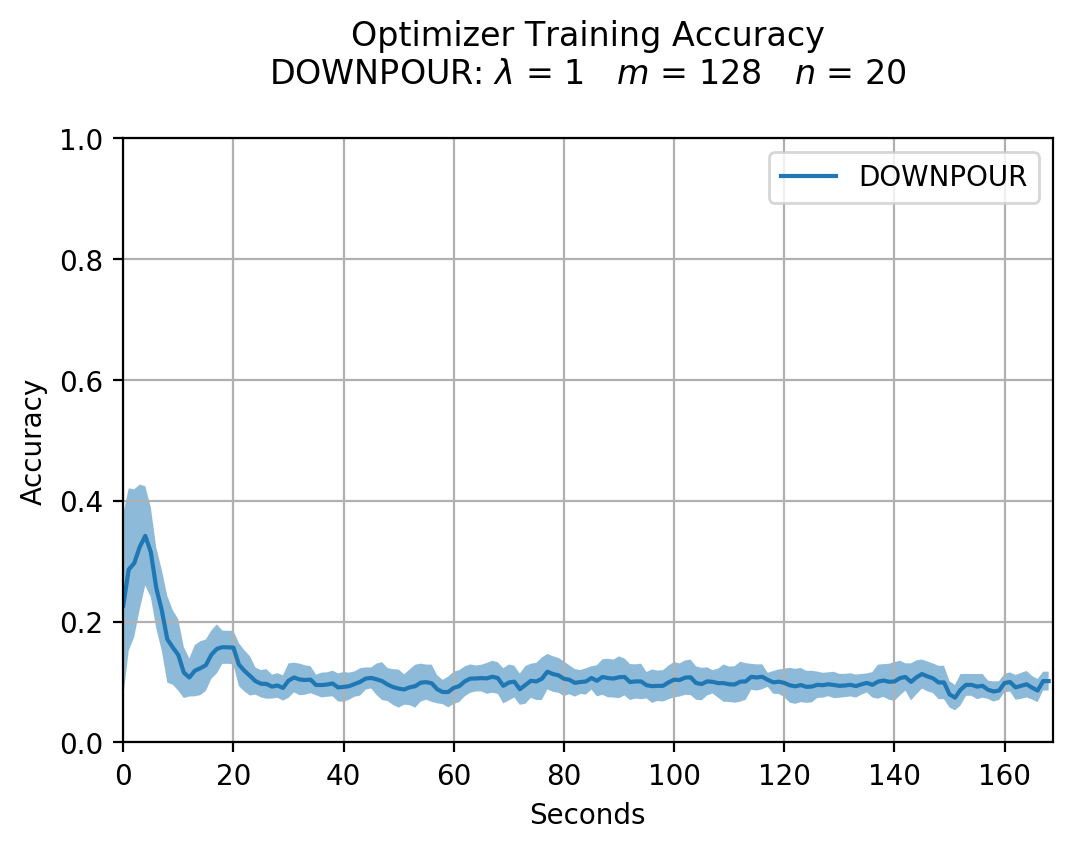
\includegraphics[width=\linewidth]{resources/images/downpour_20}
    \caption{$n = 20$}
  \end{subfigure}
  \caption{Divergence due to number ($n = 20$) of asynchronous workers in the optimization process~\cite{implicitmomentum} and not dealing with parameter staleness in a more intelligent way. Lowering the number workers ($n = 10$) causes the central variable to converge.}
  \label{fig:downpour_convergence}
\end{figure}


\subsection{Dynamic SGD}
\label{sec:dyn_sgd}

\subsection{Asynchronous Elastic Averaging SGD}
\label{sec:aeasgd}

\section{Hybrids}
\label{sec:hybrids}

% Chapter on Asynchronous Distributed Adaptive Gradient
%
% Developed for my Master Thesis at Maastricht University.
% Based on Eugenio Senes's template at the University of Torino.
%
% By Joeri Hermans (joeri@joerihermans.com)
%
% Released under an MIT license. Share, modify and enjoy, but quote the author!

\chapter{Accumulated Gradient Normalization}
\label{chapter:accumulated_gradient_normalization}

This chapter addresses the first contribution of this thesis, which is \emph{accumulated gradient normalization}, or \textsc{agn} in short. We start by laying out the concept and intuition behind accumulated gradient normalization, and show why \textsc{agn} provides the central variable with more efficient updates. Finally, to show our claims, we provide several experiments where we compare \textsc{agn} with different distributed optimizers such as \textsc{donwpour}~\cite{dean2012large}, \textsc{aeasgd}~\cite{zhang2015deep}, and \textsc{dynsgd}~\cite{jiang2017heterogeneity}.

\section{Concept and intuition}
\label{sec:agn_concept}

The main issue with \textsc{downpour}~\cite{dean2012large} is the requirement of constant communication with the parameter server after every gradient computation. Furthermore, as the number of parallel workers increases, \textsc{downpour} fails to converge due to the amount of \emph{implicit momentum}~\cite{implicitmomentum}, as shown in Figure~\ref{fig:downpour_convergence}. To reduce the amount of communication with the parameter server, one could take ideas from \textsc{easgd}~\cite{zhang2015deep}, and perform several iterations of local exploration before committing the gradients to the parameter server. However, in the case of algorithms like \textsc{downpour}, that is, where gradients are committed to the parameter server in an asynchronous fashion, more local exploration results in proportionally larger gradients, and as a result, complicate the staleness and the implicit momentum problem even further as will be addressed in Chapter~\ref{chapter:asynchronous_distributed_adaptive_gradients}. To intuitively show why this is an issue, let us consider Figure~\ref{fig:downpour_accumulation_issue}. In a regular \textsc{downpour} setting, first-order gradients such as in Subfigure (a) are committed to the parameter server. However, when an algorithm allows for a certain amount of local exploration, such as Algorithm~\ref{algo:downpour_worker_zealous}, the gradient that is committed to the parameter server is an \emph{accumulated gradient} as shown in Subfigure (b).

\begin{figure}[H]
  \centering
  \begin{subfigure}{.49\textwidth}
    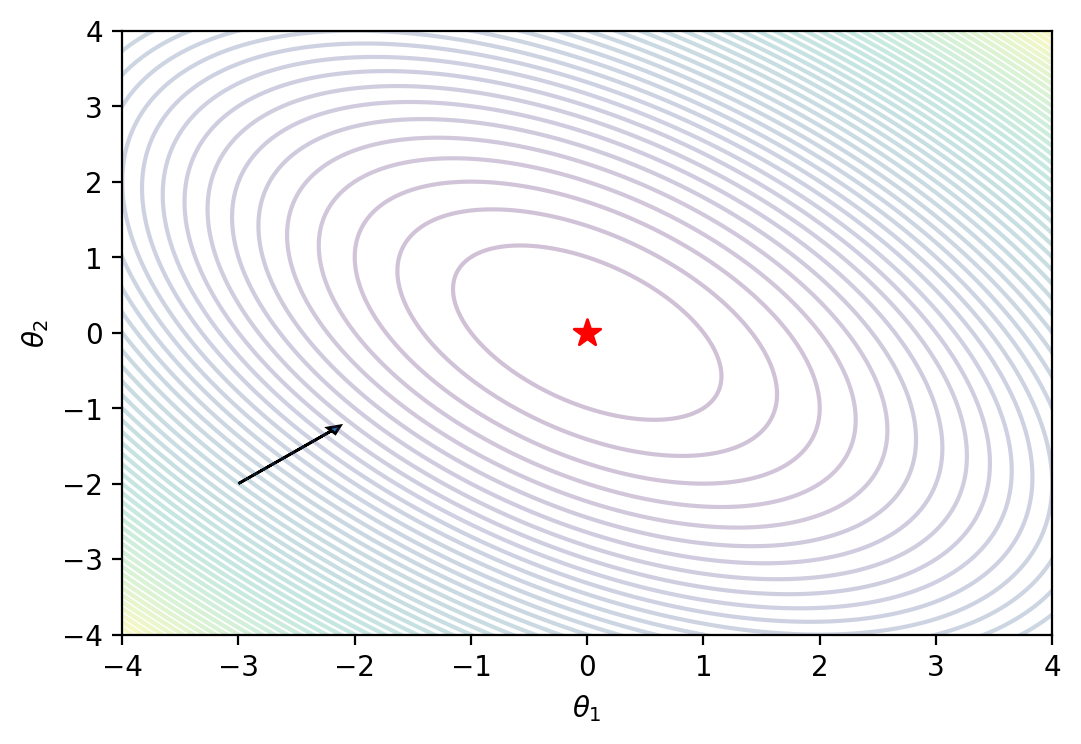
\includegraphics[width=\linewidth]{resources/images/agn_no_accumulated}
    \caption{No Gradient Accumulation}
  \end{subfigure}
    \begin{subfigure}{.49\textwidth}
    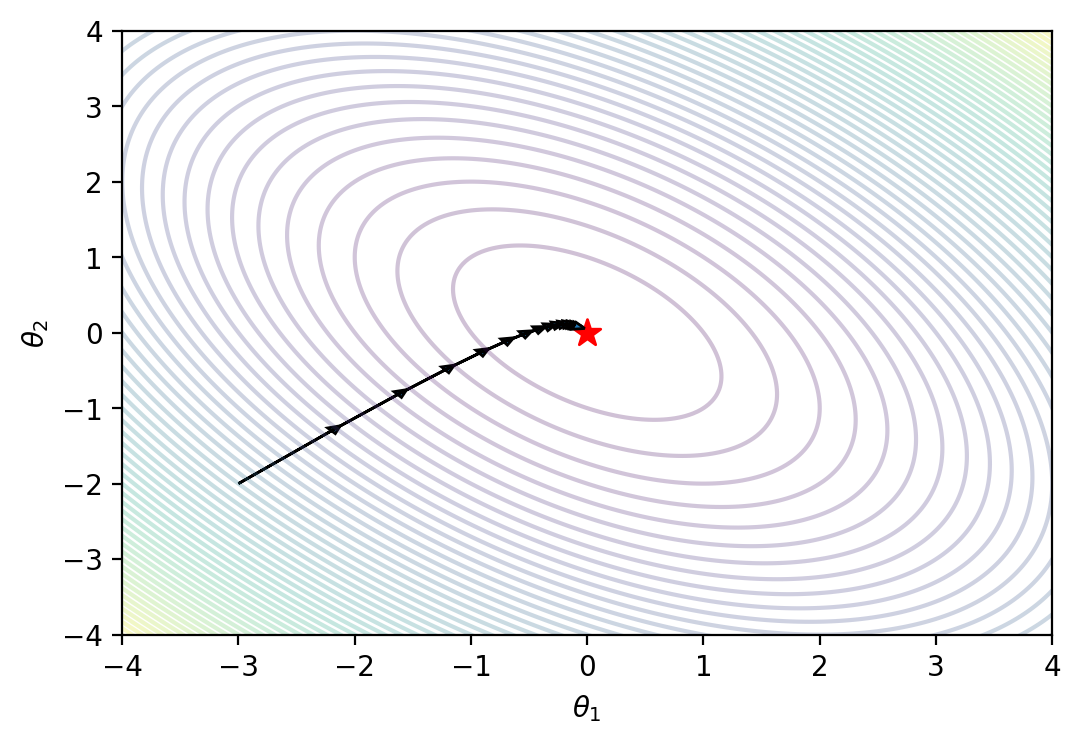
\includegraphics[width=\linewidth]{resources/images/agn_accumulated}
    \caption{Gradient Accumulation}
  \end{subfigure}
  \caption{This figure shows the difference between regular first-order gradients (a), and accumulated gradients (b). We observe that \emph{accumulated gradients are proportionally larger to the number of exploration steps}. However, they do provide a better direction compared to first-order gradients.}
  \label{fig:downpour_accumulation_issue}
\end{figure}

Now, imagine two asynchronous environments, in the first no gradient accumulation is performed, and in the last gradient accumulation takes place. In the environment where no gradient accumulation is performed, as in regular \textsc{downpour}, first-order gradients are committed to the parameter server. However, as we have seen in Chapter~\ref{chapter:distributed_deep_learning}, and in particular Figure~\ref{fig:downpour_convergence}, we saw that \textsc{downpour} diverges when the number of asynchronous workers is too high due to the amount of implicit momentum~\cite{implicitmomentum}. As a result, careful tuning is required when no adaptive methods are applied. Nevertheless, given the fact that \textsc{downpour} converges with $n = 10$ workers in Figure~\ref{fig:downpour_convergence} and our knowledge about gradient accumulation, i.e., \emph{accumulated gradients that are committed are proportional to the number of exploration steps for every worker, and provide better directions to a minimum}, we would expect that for some amount of local exploration while using the same hyperparameterization (with the exception of local exploration steps $\lambda$) \textsc{downpour} would diverge again due to the magnitude of the accumulated gradients. This behaviour is illustrated in Figure~\ref{fig:downpour_accumulated_divergence}.\\

\begin{figure}[H]
  \centering
  \begin{subfigure}{.49\textwidth}
    \centering
    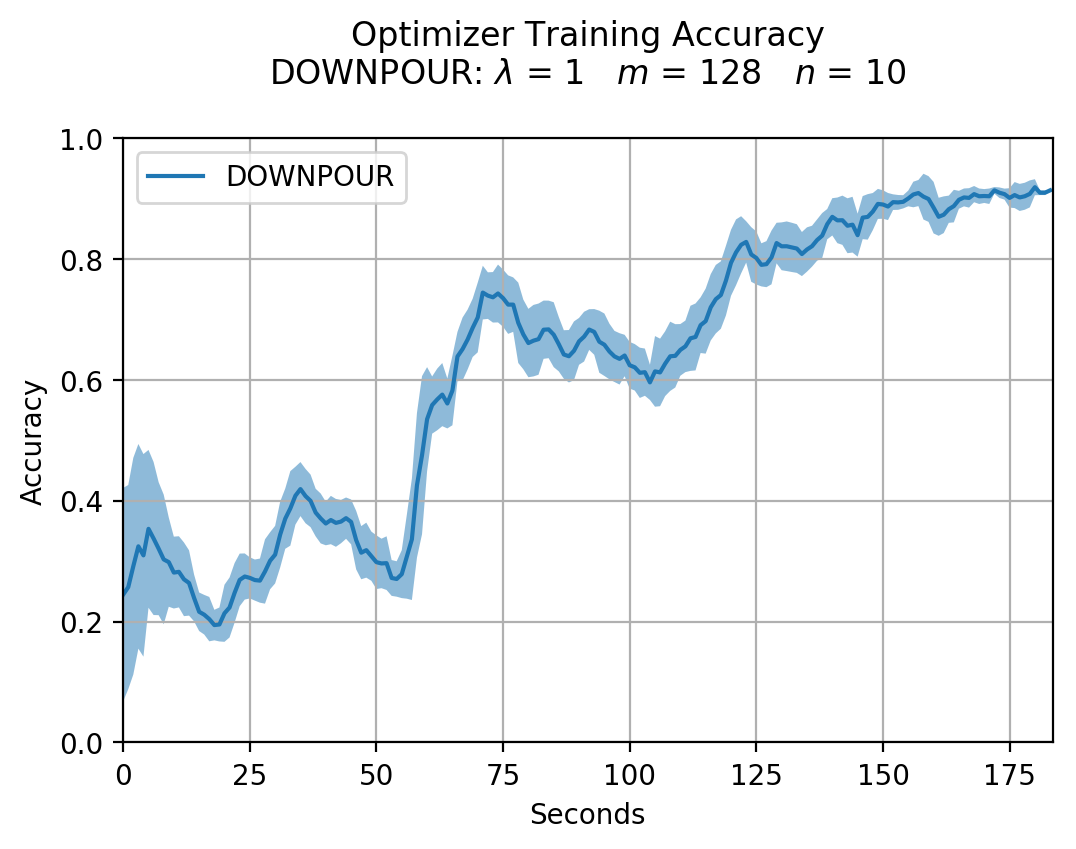
\includegraphics[width=\linewidth]{resources/images/downpour_10}
    \caption{$\lambda = 1$}
  \end{subfigure}
  \begin{subfigure}{.49\textwidth}
    \centering
    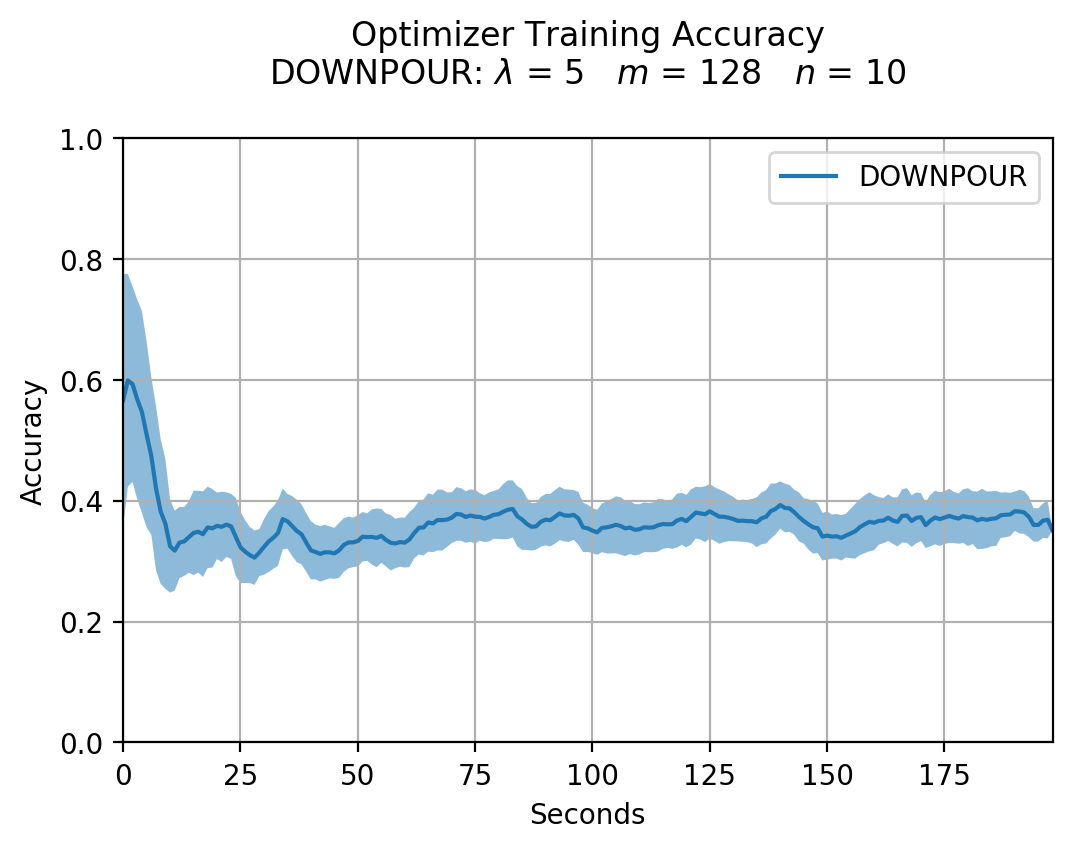
\includegraphics[width=\linewidth]{resources/images/downpour_accumulated_5}
    \caption{$\lambda = 5$}
  \end{subfigure}
   \begin{subfigure}{.49\textwidth}
    \centering
    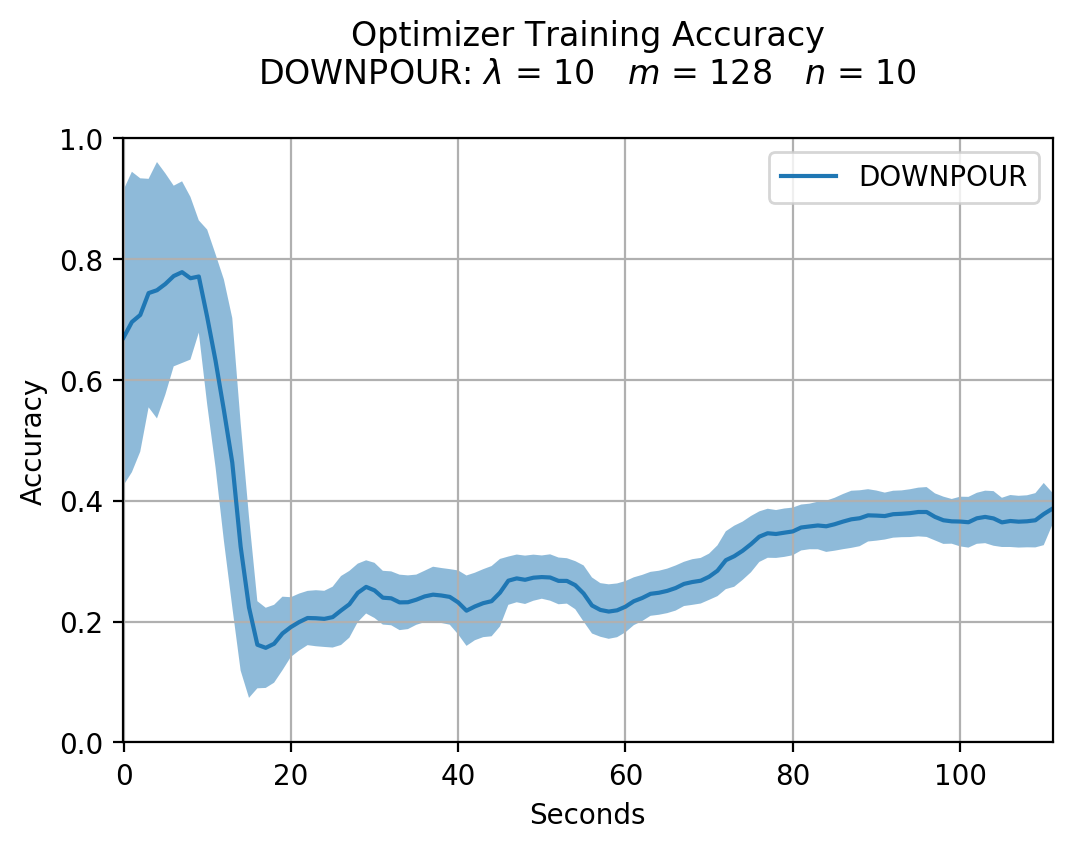
\includegraphics[width=\linewidth]{resources/images/downpour_accumulated_10}
    \caption{$\lambda = 10$}
  \end{subfigure}
  \begin{subfigure}{.49\textwidth}
    \centering
    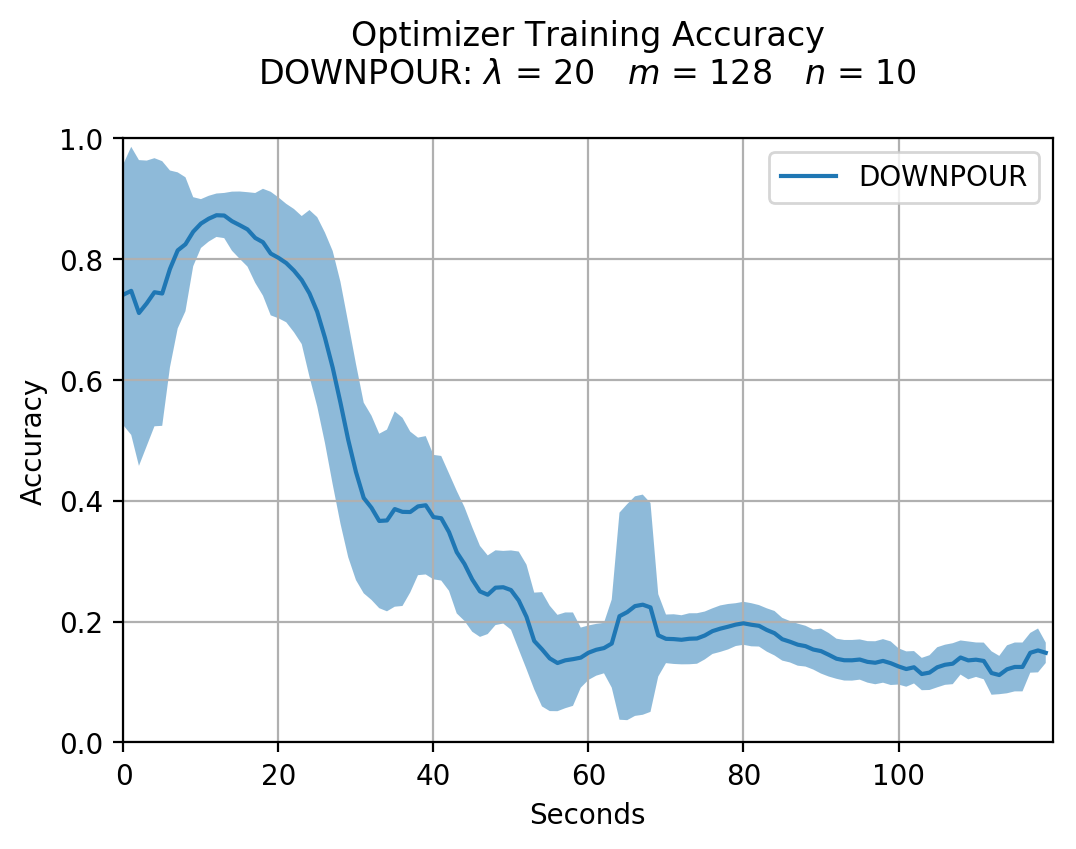
\includegraphics[width=\linewidth]{resources/images/downpour_accumulated_20}
    \caption{$\lambda = 20$}
  \end{subfigure}
  \caption{Illustration of divergence due to gradient accumulation in \textsc{downpour}. In Figure~\ref{fig:downpour_convergence}, we say that for $n = 10$ \textsc{downpour} converged to a good solution. In order to reduce the training time, we decrease the communication frequency (increasing $\lambda$). However, due to the larger gradients that are committed to the parameter server, which increases the amount of implicit momentum, the central variable is not able to converge as before.}
  \label{fig:downpour_accumulated_divergence}
\end{figure}

To reduce the magnitude of the accumulated gradients, and thereby reducing the amount of implicit momentum, while at the same time preserving the better direction that has been provided due to the amount of local exploration, we propose to normalize (average) the accumulated gradient with the amount of local steps that have been performed by the workers ($\lambda$), shown in Equation~\ref{eq:accumulated_gradient_normalization}\footnote{Note if $\lambda = 1$, \textsc{agn} is in essence equivalent to \textsc{downpour}.}. We call this technique of normalizing the accumulated gradient \emph{Accumulated Gradient Normalization} or \textsc{agn}. An initial critique of this technique would be that by normalizing the accumulated gradient, \textsc{agn} would in effect be undoing the work that has been done by a single worker. This seems at first a valid criticism, however, one needs to take into account that \textsc{agn} is actually using the worker exploration steps to compute a better gradient based on first-order gradients.

\begin{equation}
  \label{eq:accumulated_gradient_normalization}
  \Delta\theta = -\frac{1}{\lambda}\sum_{i = 0}^\lambda \eta_t \frac{1}{m}\sum_{j = 0}^{m - 1} \nabla_\theta \mathcal{L}(\theta_i;x_{ij};y_{ij})
\end{equation}

Since \textsc{agn} is using local steps to compute a better gradient compared to first order gradients, it can also be used under communication constraints like \textsc{easgd} since less communication with the parameter server is required. In Figure~\ref{fig:agn_example}, we show how a \emph{Normalized Accumulated Gradient} is obtained and applied to the central variable using Equation~\ref{eq:accumulated_gradient_normalization} as described in Algorithm~\ref{algo:agn}.

\begin{figure}[H]
  \centering
  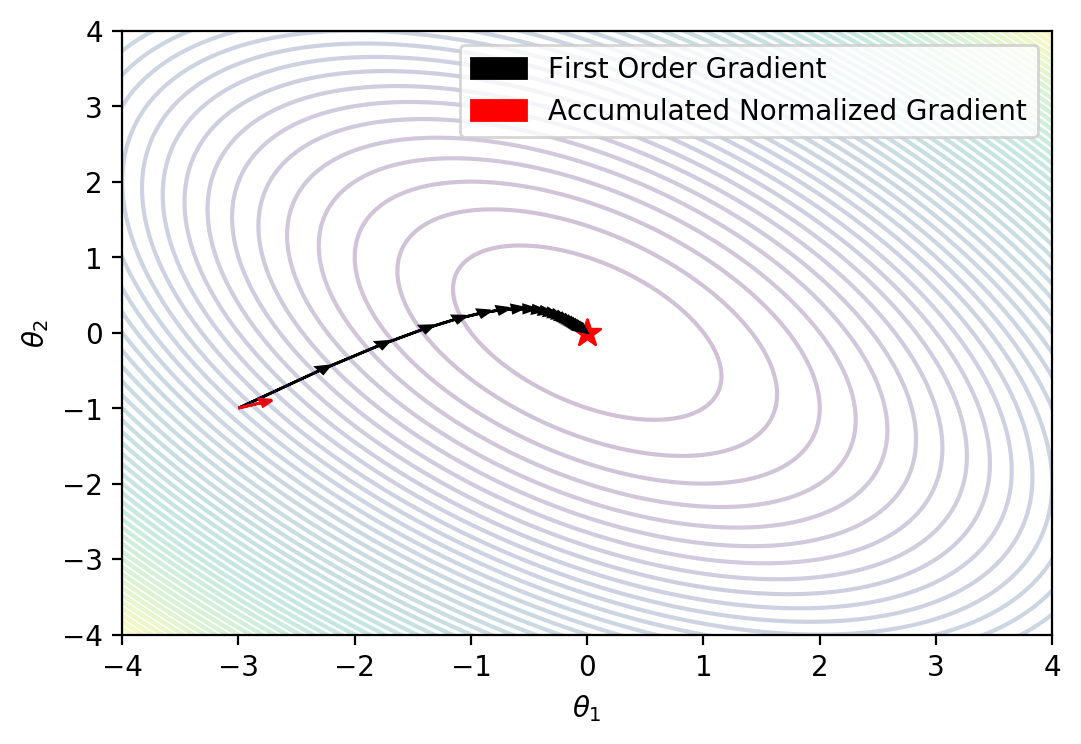
\includegraphics[width=.45\textwidth]{resources/images/agn_example}
  \caption{After pulling the most recent parameterization of the central variable from the parameter server, the worker starts accumulating $\lambda$ first order gradients, and applies those gradients locally to explore the surrounding error space. Finally, after $\lambda$ exploration steps have been performed, the accumulated is normalized w.r.t. $\lambda$ and send to the parameter server.}
  \label{fig:agn_example}
\end{figure}

\begin{algorithm}[H]
  \caption{Worker procedure of \textsc{agn}.}
  \label{algo:agn}
  \begin{algorithmic}[1]
    \Procedure{AGNWorker}{$k$}
    \State $\theta^k_0 \gets \tilde{\theta} \gets \Call{Pull}$
    \State $t \gets 0$
    \While{$\textbf{not}$ converged}
    \State $i \gets 0$
    \State $a \gets 0$
    \While{$i < \lambda$}
    \State $\textbf{x},~\textbf{y} \gets \Call{FetchNextMiniBatch()}{}$
    \State $g \gets -\eta_t \odot \nabla_\theta \mathcal{L}(\theta^k_t;\textbf{x};\textbf{y})$
    \State $a \gets a + g$
    \State $\theta^k_{t + 1} = \theta^k_t + g$
    \State $i \gets i + 1$
    \State $t \gets t + 1$
    \EndWhile
    \State $a \gets \frac{a}{\lambda}$ \Comment{Accumulated Gradient Normalization step.}
    \State $\Call{Commit}{a}$
    \State $\theta^k_{t} \gets \Call{Pull}$
    \EndWhile
    \EndProcedure
  \end{algorithmic}
\end{algorithm}

An interesting thought experiment would be what would happen in the case that the workers would not communicate with the parameter server at all, that is, $\lambda = \infty$. How would the normalized accumulated gradients look like in such a situation, described by Equation~\ref{eq:agn_thought_experiment}?

\begin{equation}
  \label{eq:agn_thought_experiment}
  \lim_{\lambda \to \infty} -\frac{\sum_{i = 0}^\lambda \eta_t \frac{1}{m}\sum_{j = 0}^{m - 1} \nabla_\theta \mathcal{L}(\theta_i;x_{ij};y_{ij})}{\lambda}
\end{equation}

In order to completely understand how the worker deltas would look like after $\lambda = \infty$ steps, one first needs to understand the individual components of Equation~\ref{eq:agn_thought_experiment}. The most inner component, $\eta_t \frac{1}{m}\sum_{j = 0}^{m - 1} \nabla_\theta \mathcal{L}(\theta_i;x_{ij};y_{ij})$, is just the computation of a mini-batch using $m - 1$ samples, where index $i$ denotes the current step in the gradient accumulation. Please note that a mini-batch can differ for different values of $i$ as training samples are randomly retrieved from the dataset. After computing the gradient based on the mini-batch, the local model will be updated as $\theta_{i + 1} = \theta_i - \eta_t\frac{1}{m}\sum_{j = 0}^{m - 1} \nabla_\theta \mathcal{L}(\theta_i;x_{ij};y_{ij})$. This process goes on for $\lambda$ steps, while at the end, the accumulated is normalized with respect to $\lambda$.\\

Let us assume we have a smooth convex error space, or a smooth non-convex error space with at least a single minima. Due to the existence of a minima in both cases, first order gradients will eventually converge to, or in the neighbourhood of said minima. Furthermore, we  make the assumption that the hyperparameterization during the training procedure will not change. For instance, no learning rate decay after $x$ number of steps. Under these assumptions, it is trivial to realize that applying gradient descent for $\infty$ steps will cause the parameterization to converge in a minima. Of course, given that the hyperparameterization, and the data allow for convergence to occur. As a result, the term $\sum_{i = 0}^\lambda \eta_t \frac{1}{m}\sum_{j = 0}^{m - 1} \nabla_\theta \mathcal{L}(\theta_i;x_{ij};y_{ij})$ is finite, even after applying $\infty$ steps of mini-batch updates. To simplify our problem, let us denote $\vec{c}$ as the \emph{finite} result of the top term in Equation~\ref{eq:agn_thought_experiment} for $\lambda = \infty$. Therefore, we can write Equation~\ref{eq:agn_thought_experiment} as Equation~\ref{eq:agn_thought_experiment_2}. Furthermore, since $\vec{c}$ is finite, Equation~\ref{eq:agn_thought_experiment_2} can be treated as an instance of $\frac{1}{\infty}$, which approaches 0. Subsequently, Equation~\ref{eq:agn_thought_experiment_2} is 0 in the limit to infinity.

\begin{equation}
  \label{eq:agn_thought_experiment_2}
  \lim_{\lambda \to \infty} - \frac{\vec{c}}{\lambda} = \vec{0}
\end{equation}

This implies that due to the infinitely low communication frequency, the normalized accumulated gradients will basically be $\vec{0}$. However, what is interesting is that the normalized accumulated gradients directly point towards a minima due to the infinite amount of exploration steps that have been performed. Subsequently, one can view a normalized accumulated gradient when $\lambda = \infty$ as a point, but with a direction. Therefore, if we would allow for infinite steps until convergence, the path the central variable would traverse is a straight line towards the minima, as shown in Figure~\ref{fig:agn_straight_line}.

\begin{figure}[H]
  \centering
  \begin{subfigure}{.49\textwidth}
    \centering
    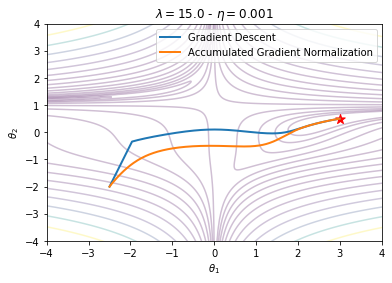
\includegraphics[width=\linewidth]{resources/images/agn_straight_line_1}
    \caption{$\lambda = 15$}
  \end{subfigure}
  \begin{subfigure}{.49\textwidth}
    \centering
    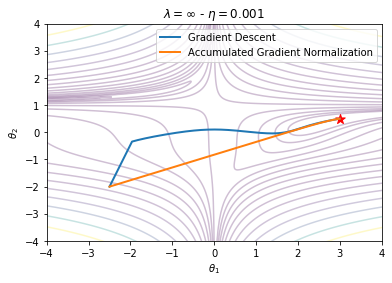
\includegraphics[width=\linewidth]{resources/images/agn_straight_line_2}
    \caption{$\lambda = \infty$}
  \end{subfigure}
  \caption{\textsc{agn} for different values of $\lambda$. This small experiment shows that when $\lambda = \infty$, the path the central variable traverses is equal to a straight line towards the minima.}
  \label{fig:agn_straight_line}
\end{figure}

The thought experiments described above helps us in several ways if make make several additional assumptions. The first assumption assumes that normalized accumulated gradients with $\lambda = \infty$ can be computed immediately, that is, without a delay. This is of course an unrealistic assumption. However, one needs to consider realistic communication constraints. Given a certain network throughput, what is the amount of local communication that needs to be performed in order for a parameter commit to be ``worth it''. As mentioned above, $\lambda = \infty$ is not a very good solution since the normalized accumulated gradient will converge to $\vec{0}$ in the limit. Nevertheless, if the normalized accumulated gradient could be computed immediately, as we assumed, the central variable would traverse the shortest path to a minima, in contrast to first order gradients. Of course, this is not a realistic assumption. Furthermore, this issue is quite similar to \emph{stochastic gradient descent} vs. \emph{mini-batch gradient descent}, since in \textsc{agn} we also have to make the decision between more frequent parameter updates, and more ``local'' iterations to compute a better gradient, where better in the case of mini-batch gradient descent means less-noisy.\\

In most settings, the size of a mini-batch is determined empirically, and is dependent on the noise of the gradients. Furthermore, when using mini-batch gradient descent, a trade-off is made between more frequent parameter updates, i.e., a smaller mini-batch, or more robust and consistent gradients by increasing the size of a mini-batch which results in a more accurate approximation of the first order curvature. This is similar to our situation. Yet, in mini-batch gradient descent you are basically trying to estimate a hyperparameter based on several unknowns, i.e., convergence based on error space and noise of individual gradients. However, \textsc{agn} is balancing the amount of local computation to produce a better gradient, with the throughput of the network, which is a known variable. For instance, imagine a hypothetical communication infrastructure which is able to apply the commits of the workers directly into the workers with no delay. In this situation, one could apply \textsc{downpour}. However, remember from Figure~\ref{fig:downpour_accumulated_divergence} that \textsc{downpour} does not handle an increased amount of asynchronous parallelism ($n = 20$). As a result, even in an ideal situation \textsc{downpour} will not be able to converge due to the amount of implicit momentum.\\

Nevertheless, the situation in \textsc{agn} is different as will become apparent in Section~\ref{sec:agn_experimental_validation}. Contrary to \textsc{downpour}, \textsc{agn} does not commit first order gradients to the parameter server, but rather a normalized sequence of first order gradients which result in better directions towards a minima, as discussed above. Because of this, workers will produce a better gradient in terms of direction with respect to first order gradients using the amount of local computation available to them to handle the communication constraints. Therefore, \textsc{agn} worker deltas will therefore point more or less in the same direction, and are normalized with respect to the number of exploration steps, which reduces the amount of implicit momentum since first order gradients are not applied to the central variable.

\section{Experimental Validation}
\label{sec:agn_experimental_validation}

In this Section we evaluate \textsc{agn} against different distributed optimization algorithms. As before, MNIST~\cite{mnist} is used as a benchmark dataset, and all optimizers use the model described in Appendix~\ref{appendix:mnist_model} with identical parameterization of the weights. Furthermore, we will set the mini-batch size to $m = 128$ in all optimizers, and use \emph{40 epochs} worth of training data that will be equally distributed over all $n$ workers with the exception for \textsc{downpour}, which will only use 5 epochs, since \textsc{downpour} can not handle accumulated gradients. Our computing infrastructure consists a relatively small cluster of \emph{15 nodes} with a \emph{10Gbps interconnect}, most of them in the same rack, each having 2 Intel\textsuperscript{\textregistered} Xeon\textsuperscript{\textregistered} CPU E5-2650 v2 @ 2.60GHz CPU's, where every CPU has 8 cores and 2 threads. No GPU's are used during training, and no learning rate decay is applied.\\

Our initial experiment, shown in Figure~\ref{fig:agn_experiment_1}, shows the training accuracy of \textsc{agn}, \textsc{aeasgd}, and \textsc{dynsgd} over time. In this experiment, we use a near-optimal hyperparameterization for all optimizers to ensure convergence. Furthermore, we also report the validation accuracy of every trained model based on the validation set that is provided by MNIST. Looking at Figure~\ref{fig:agn_experiment_1}, we observe a significant increase in training performance for \textsc{agn}, both in training accuracy, and in training time when compared to current state-of-the-art algorithms such as \textsc{aeasgd} and \textsc{dynsgd}. Furthermore, the claim we made in Chapter~\ref{chapter:distributed_deep_learning} that \textsc{dynsgd} scales the gradients down with respect to staleness $\tau$, which in effect is $\textbf{E}[\tau] = n - 1$, and thereby not addressing the staleness problem since the expected scaling factor is $(n - 1)^{-1}$ and not the distance between the parameterization of the central variable, and the parameterization of the worker, can be derived from Figure~\ref{fig:agn_experiment_1} and Figure~\ref{fig:agn_experiment_1} (b). Since gradient accumulation is performed in both figures, i.e., $\lambda > 1$, we can tell that \textsc{dynsgd} has difficulties converging when $\lambda$ is larger because the gradients that are committed to the parameter server are proportionally larger, as is the case in Figure~\ref{fig:agn_experiment_1} (a). Furthermore, due to the relatively high communication frequency ($\lambda = 10$), \textsc{dynsgd} will take longer to process all data since more communication with the parameter server is required. However, in the case of Figure~\ref{fig:agn_experiment_1} (a), we see that \textsc{dynsgd} is equally \emph{temporal efficient} to \textsc{aeasgd}, since \textsc{dynsgd} takes the \emph{same} amount of time to reach the final training accuracy of \textsc{aeasgd}.

\begin{figure}[H]
  \centering
  \begin{subfigure}{.49\textwidth}
    \centering
      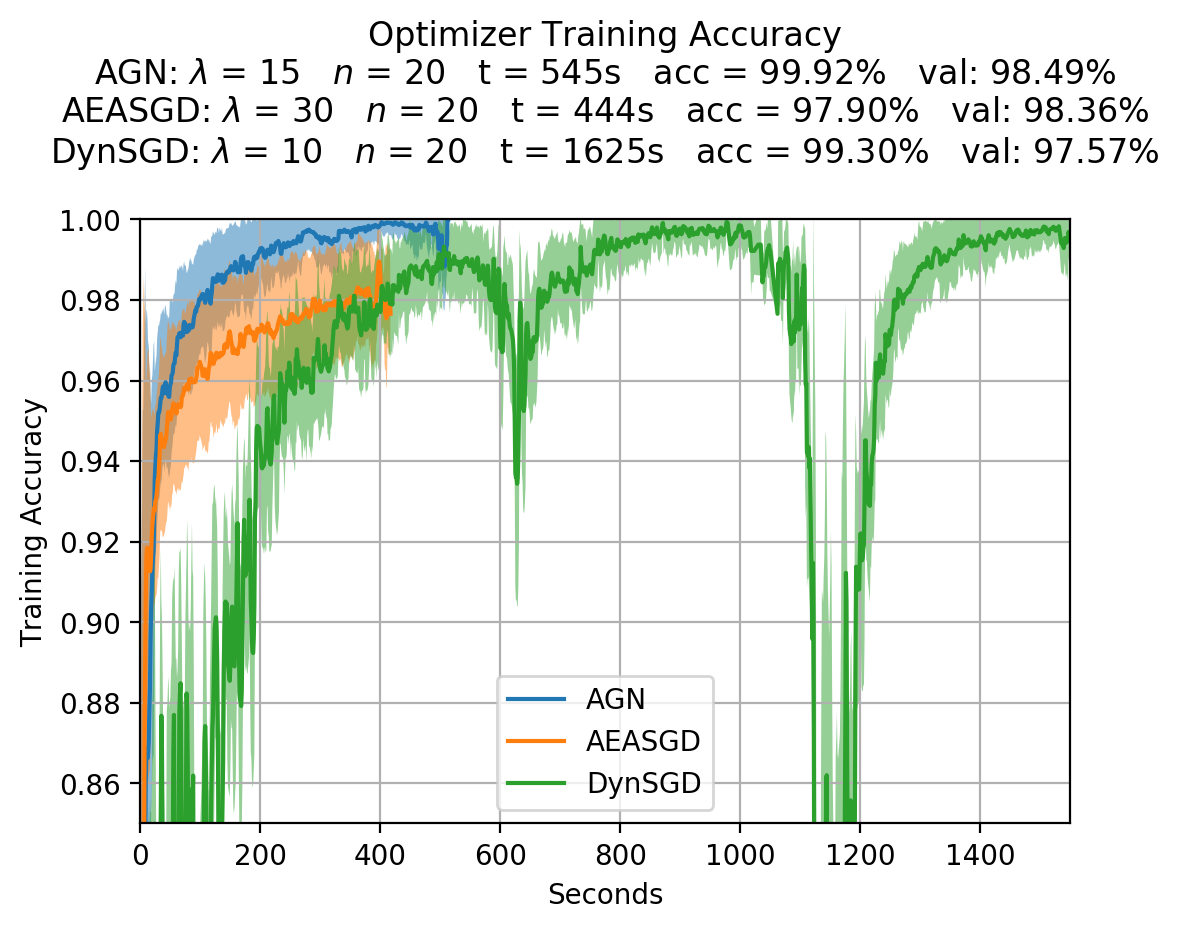
\includegraphics[width=\textwidth]{resources/images/agn_experiment_1}
      \caption{\textsc{dynsgd} $\lambda = 10$}
  \end{subfigure}
  \begin{subfigure}{.49\textwidth}
    \centering
      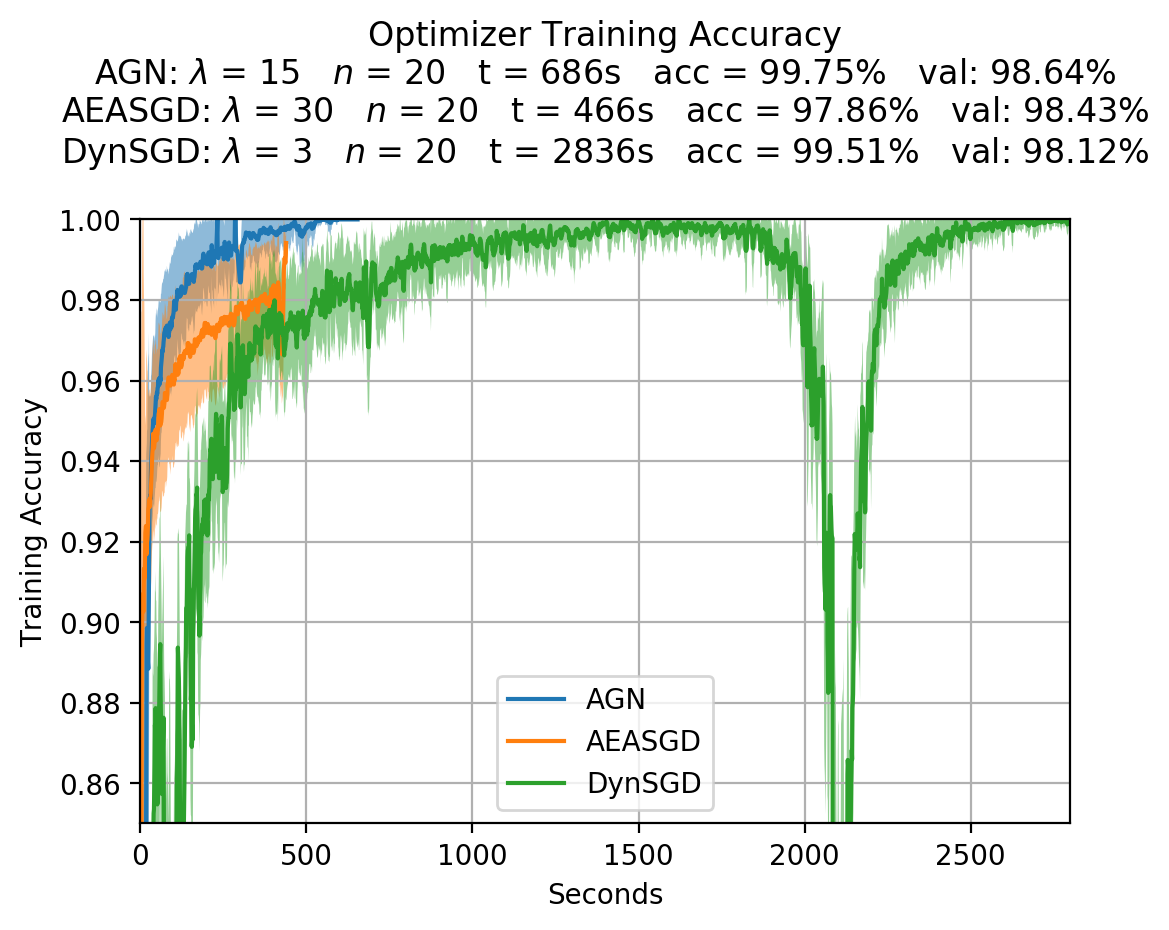
\includegraphics[width=\textwidth]{resources/images/agn_experiment_2}
      \caption{\textsc{dynsgd} $\lambda = 3$}
  \end{subfigure}
  \caption{In this experiment we train all optimizers on 40 epochs worth of data with a mini-batch of $m = 128$. Due to staleness-handling method of \textsc{dynsgd}, the optimizer is not able to handle accumulated gradients which results in non-stale accumulated gradients being incorperated directly into the central variable with the disadvantage that other workers are even more stale in terms of parameter distance. Which is the root cause of this divergent behaviour. In Subfigure (b) we reduce the amount of local exploration steps, which in turn reduces the length of the accumulated gradient. Therefore causing other workers to be less stale, and consequently reducing the divergent effects we observed in Subfigure (a). Furthermore, in Chapter~\ref{chapter:distributed_deep_learning}, we made that claim that \textsc{aeasgd} will not be able to get close to a minima due to the existence of an equilibrium. This behaviour is confirmed as \textsc{aeasgd} is not able to surpass \textsc{agn} in terms of training accuracy. However, as mentioned in Chapter~\ref{chapter:distributed_deep_learning}, the validation accuracy of \textsc{aeasgd} is usually higher than the training accuracy. This results further strengthens our suggestion that due to the presence of the equilibrium condition, \textsc{aeasgd} will not overfit the data since the optimizer will not be able to come ``close'' to a minima.}
  \label{fig:agn_experiment_1}
\end{figure}

Furthermore, let us consider the case for \textsc{dynsgd} when $\lambda = 15$. In this situation, \textsc{dynsgd} closely resembles \textsc{agn} since, as mentioned above, the worker deltas in \textsc{dynsgd} are scaled down with respect to the staleness $\tau$, which results in an expected scaling factor of $(n - 1)^{-1}$. Whereas in \textsc{agn}, the deltas are always scaled (on worker level) with respect to the communication frequency $\lambda$. As a result, the scaling of worker deltas will be \emph{on average} similar to \textsc{agn}. This begs the question, why do we see such divergent, and noisy behaviour in Figure~\ref{fig:agn_experiment_1}, and especially in Figure~\ref{fig:agn_experiment_2}? The reason for the lies in the combined effect how \textsc{dynsgd} deals with staleness, and due to the precense of gradient accumulation. To illustrate this behaviour, consider the case when a \textsc{dynsgd} worker $w$ is committing an \emph{accumulated gradient}, with staleness 0, i.e., $\tau_w = 0$. In this situation, the parameter server will scale down the gradient with respect to $(0 + 1)^{-1}$, which is 1. As a result, the accumulated gradient that worker $w$ sent to the parameter server will not be scaled down. Of course, this is perfectly reasonable, since there the accumulated gradient that worker $w$ sent was not stale. However, what happens when the other $n - 1$ workers have to commit a gradient? Remember from Equation~\ref{eq:dynsgd_ps} that \textsc{dynsgd} scales the gradients down with respect to the number of \emph{stale steps} $\tau_w$. As we will show in Chapter~\ref{chapter:asynchronous_distributed_adaptive_gradients}, this method is rather naive, because what really matters is the \emph{distance} between updates as suggested in Hypothesis~\ref{hyp:local_optimization}. Since the delta worker $w$ committed was not stale, the full accumulated gradient was incorperated into the central variable, causing it to shift with the full magnitude of the delta. Since the length of an accumulated gradient is proportional to the number of local exploration steps, the deltas of other workers will be proportionally more stale in terms of distance, and therefore causing the divergent behaviour shown in Figure~\ref{fig:agn_experiment_1} and Figure~\ref{fig:agn_experiment_2}.

\begin{figure}[H]
  \centering
  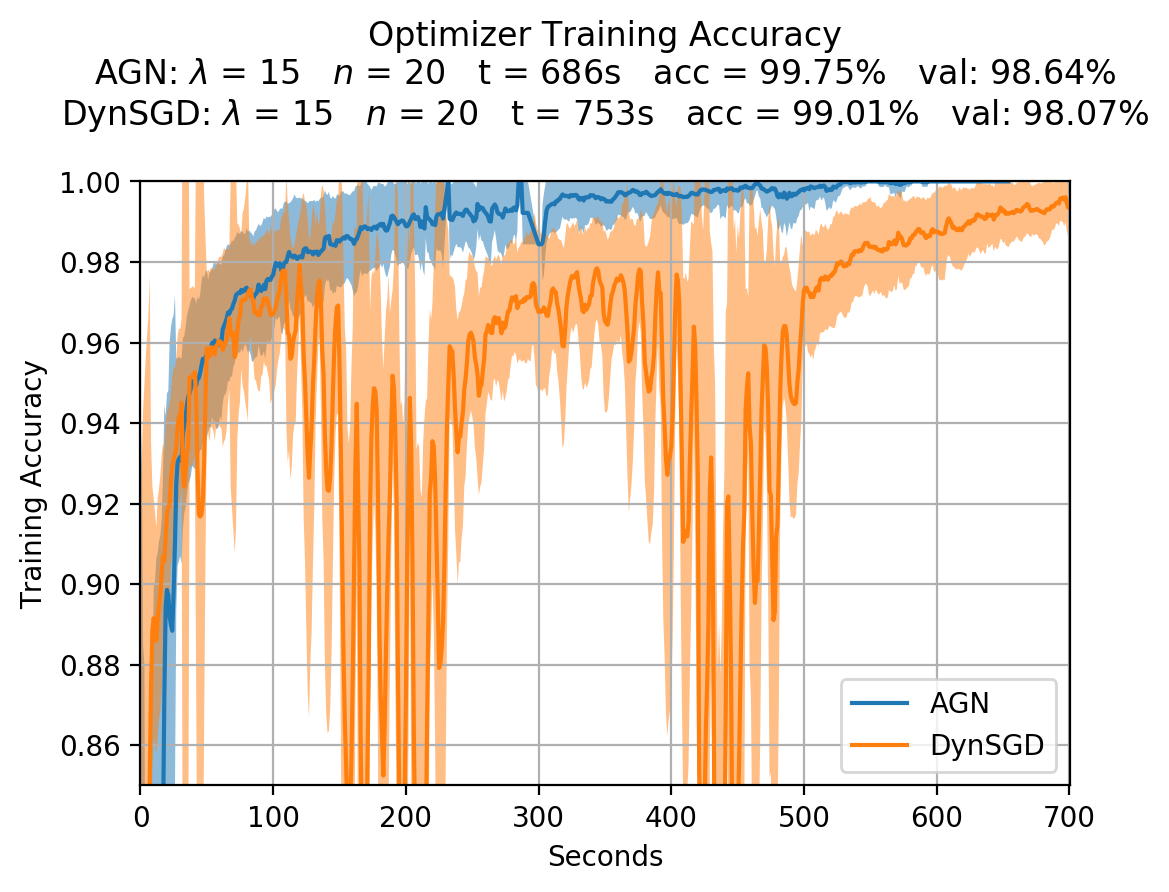
\includegraphics[width=.6\textwidth]{resources/images/agn_experiment_3}
  \caption{Shows the similarity between \textsc{agn} and \textsc{dynsgd} by using identical communication frequencies in both optimizers. As a result, \textsc{dynsgd} worker deltas are \emph{expected} to be similar to \textsc{agn} deltas since $\textbf{E}[\tau] = n - 1$. However, due to \textsc{dynsgd}'s staleness handling mechanism, which is basically scaling the deltas down by the number of \emph{stale steps}, \textsc{dynsgd} is not able to prevent divergent behaviour. Contrary to \textsc{dynsgd}, \textsc{agn} is not staleness aware. However, \textsc{agn} does provide more stable and direct gradient updates since the optimizer normalizes the accumulated gradients proportionally to the amount of local exploration.}
  \label{fig:agn_experiment_2}
\end{figure}

An additional observation from Figure~\ref{fig:agn_experiment_1} and Figure~\ref{fig:agn_experiment_2}, one we made before in Chapter~\ref{chapter:distributed_deep_learning}, is that the validation accuracy of \textsc{aeasgd} is in accordance with the training accuracy, meaning, the optimizer does not seem to overfit. The reason for this lies, according to us, with the \textsc{easgd} equilibrium condition, described in Section~\ref{sec:easgd}. The equilibrium condition will prevent the central variable moving too close to a minima, preventing the central variable from overfitting. Since \textsc{aeasgd} and \textsc{agn} are clearly outperforming \textsc{dynsgd} in terms of training time and validation accuracy for this particular experiment, the following experiments will only consider \textsc{aeasgd} and \textsc{agn}. To evaluate the performance of these optimizers under different conditions, we will conduct several experiments using the same hyperparameterizations we mentioned at the start of this Section, which will evaluate the performance of \textsc{agn} and \textsc{aeasgd} with respect to different (distributed) hyperparameters, i.e., number of workers, and communication frequency. As before, no learning rate decay is applied.\\

Initial observations from our results, summarized in Table~\ref{table:agn_experiments_summary}, indicate that \textsc{agn} performes better in terms of validation accuracy when a low communication frequency is used (which is a design requirement of \textsc{(a)easgd}), and a high number of asynchronous workers are deployed ($n \geq 20$). However, looking at the overall training accuracy of both optimizers, we observe that \textsc{agn} is significantly outperforming \textsc{aeasgd} in all configurations of the distributed hyperparameters. The reason for this might be due to the equilibrium condition of \textsc{easgd} described in Chapter~\ref{chapter:distributed_deep_learning}. Furthermore, increasing the number of asynchronous workers results in a significant drop in both training, and validation accuracy in \textsc{aeasgd}.

\begin{figure}[H]
  \centering
  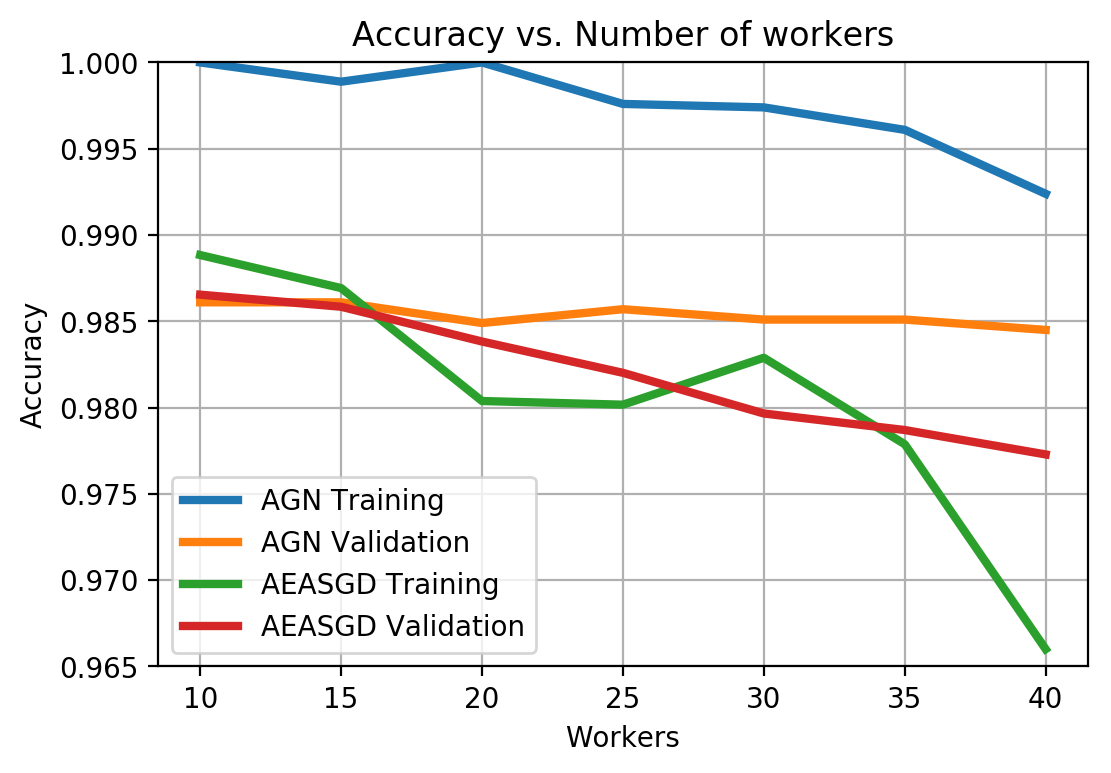
\includegraphics[width=.5\textwidth]{resources/images/agn_aeasgd_workers}
  \caption{Decline of the training accuracy of both \textsc{agn} and \textsc{aeasgd} as the number of asynchronous workers increases. From these experiments, we observe that \textsc{agn} is more rebust to an increased amount of asynchrony as the training accuracy only starts to decrease from $n = 25$ workers, while the validation accuracy remains stable even with 40 workers.}
  \label{fig:agn_aeasgd_workers_performance_decline}
\end{figure}

Contrary to \textsc{aeasgd}, \textsc{agn} is able to cope more effectively with an increased amount of parallelism, as its training accuracy only starts to decline from $n = 25$ asynchronous workers, while the validation accuracy is barely fluctuating (because \textsc{agn} is still slightly overfitting), as shown in Figure~\ref{fig:agn_aeasgd_workers_performance_decline}. An obvious follow-up question to this result would be to question the fact whether increasing the amount of asynchronous workers really improves the temporal efficiency optimizer, i.e., the amount of time it takes to reach a certain training accuracy. In fact, it does reduce the training time to reach a certain training accuracy, as shown in Figure~\ref{fig:agn_temporal_efficiency}. However, several factors have to be taken into account.

\begin{figure}[H]
  \centering
  \begin{subfigure}{.49\textwidth}
    \centering
    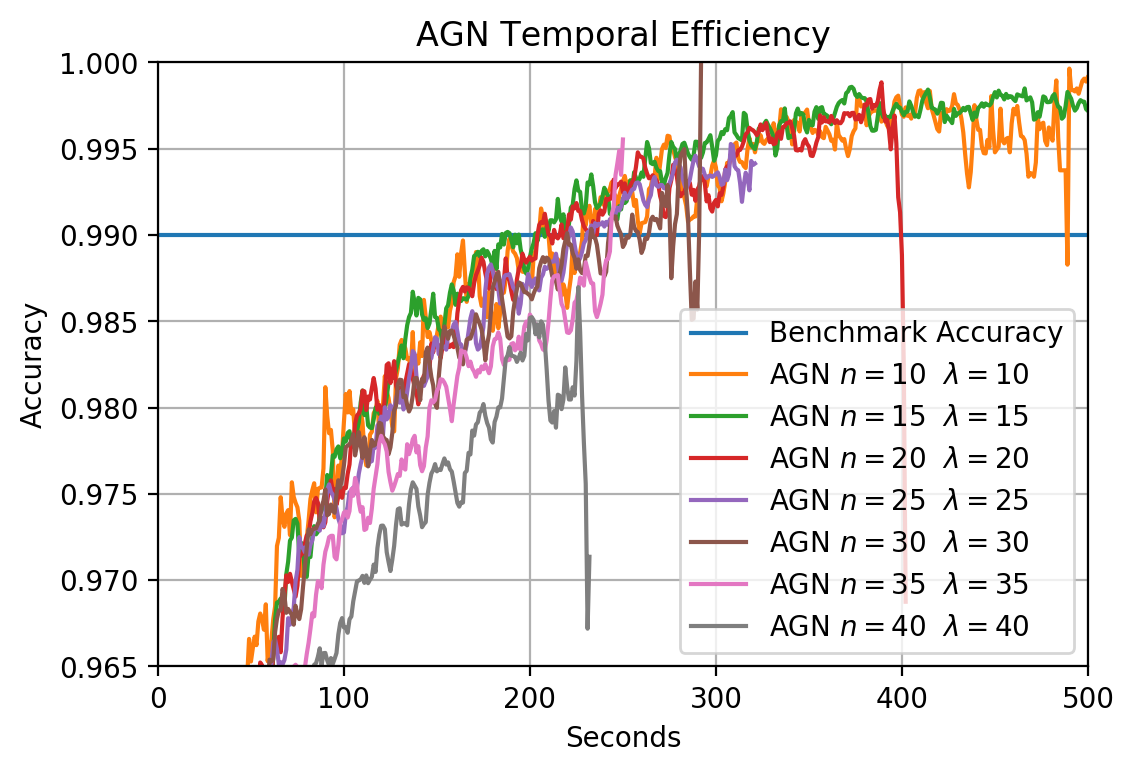
\includegraphics[width=\linewidth]{resources/images/agn_temporal_efficiency}
    \caption{Varying $\lambda$}
  \end{subfigure}
  \begin{subfigure}{.49\textwidth}
    \centering
    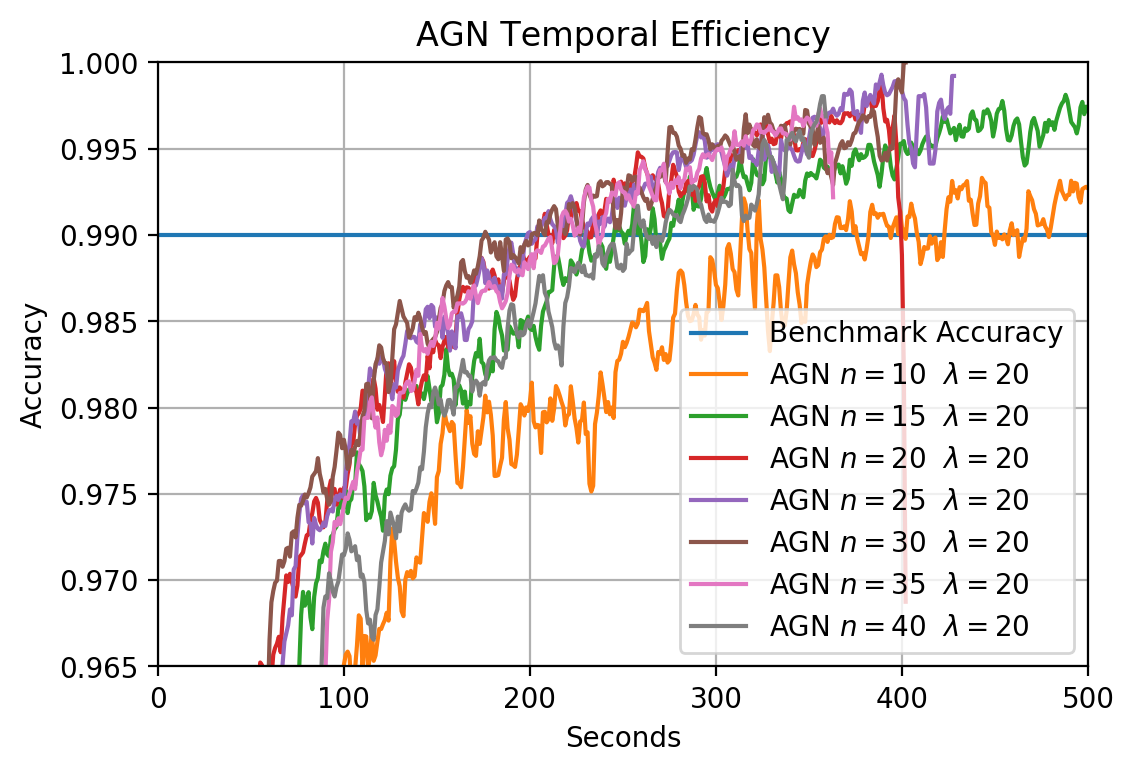
\includegraphics[width=\linewidth]{resources/images/agn_temporal_efficiency_2}
    \caption{Static $\lambda$}
  \end{subfigure}
  \caption{Training accuracy plots for different configurations of the distributed hyperparameters. In the case of a varying $\lambda$ with respect to the number of workers (to minimize the noise of the commits), we observe that optimizers with a higher communication frequency (small $\lambda$), is actually benifitting from the more frequent updates with the parameter server. However, as the number of asynchronous workers grows, a low communication frequency increases the noise in the commits due to parameter staleness. Furthermore, if the $lambda$ is too large, less frequent parameter server updates occur, which results in a slower convergence rate since more time is spent locally. As a result, a balance is required similar to determining the size of a mini-batch.}
  \label{fig:agn_temporal_efficiency}
\end{figure}

The first being an increased amount of staleness that is inserted into the system as the number of asynchronous workers increase. This effect is difficult to mitigate. Previous approaches~\cite{jiang2017heterogeneity} propose to scale gradient commits down proportionally to the number of stale steps. However, as previously shown, this is not an effective solution since accumulating gradients locally, is in effect making the gradients larger, and as a result, committing accumulated gradients increases the \emph{distance} between the central variable and other workers\footnote{Which is our definition of staleness, see Chapter~\ref{chapter:asynchronous_distributed_adaptive_gradients}}. The second and final issue is the balance between updating the central variable with a certain frequency, and the amount of local work to effectively reduce the training time due to high communication costs. In effect, this resembles the situation usually one has when selecting a mini-batch size $m$, i.e., do we allow for more frequent parameter updates (small $m$), or do we compute a less noisy first order gradient by increasing $m$, thereby reducing the frequency of parameter updates and the convergence of a model? To show that this is the case, let us consider Figure~\ref{fig:agn_experiments_workers} and Figure~\ref{fig:agn_experiments_lambdas}. In Figure~\ref{fig:agn_experiments_workers}, we evaluate varying values of $\lambda$ for a specific number of asynchronous workers $n$. In all cases, we observe configurations using $\lambda = 40$ usually have the slowest convergence rate with respect to other configurations with higher communication frequencies. Furthermore, an additional interesting observation, one which is in accordance with the theory we discuss in Chapter~\ref{chapter:asynchronous_distributed_adaptive_gradients}, is the fact that high communication frequencies and a larger number of asynchronous workers causes divergent behaviour due to parameter staleness.\\

Nevertheless, what is really interesting, is why configurations with low communication frequencies actually do converge, in contrast to configurations with high communication frequencies (with respect to the number of workers). Since our definition of staleness relates to the distance between the \emph{current} parameterization of a worker, and the \emph{current} parameterization of the central variable. One can imagine that increasing the number of asynchronous workers, effectively increases the \emph{distance} between the parameterizations of the workers and the \emph{current} central variable due to the queueing model discussed before, i.e., worker deltas are incorporated in the central variable in a queueing fashion. Yet, parameter staleness still does not explain why configurations with low communication frequencies converge, as opposed to configurations with higher communication frequencies. The question begs, is convergence guaranteed due to the amount of local exploration, thus providing the parameter server with a better ``direction'', as shown in Figure~\ref{fig:agn_example}. Or, is it due to limit condition described in Equation~\ref{eq:agn_thought_experiment_2}, which eventually scales the worker deltas down to 0 as the communication frequency decreases ($\lambda$ increases)? This is a rather difficult question to answer. However, we are definitely not dealing with the limit condition since one expects this to be the case when \textsc{agn} approaches a minima, or when $\lambda$ approaches infinity. As a result, the convergence property of \textsc{agn} is largely dedicated to the amount of local exploration, which in turn provides the central variable with a more stable, and direct gradient towards a minima. Alternatively, consider the case when no normalization of the accumulated gradient proportional to the amount of local exploration takes place, and thereby pushing large gradients to the parameter server. We showed that this approached has the tedency to diverge despite the fact it provides a better direction, as is the case in \textsc{agn}. However, due to the magnitude of the worker delta, a lot of staleness (in terms of distance) is induced causing other workers to commit (also large) gradients in an already very stale central variable, which in turn causes the divergence we observe in a non-normalized setting.\\

Now the argument on convergence rates of \textsc{agn} with respect to the communication frequency has been made, let us focus on the influence on the amount of asynchronous workers. For this, we turn to Figure~\ref{fig:agn_experiments_lambdas}, which shows the accuracy plots for several training configurations with a static communication frequency, and a varying number of asynchronous workers. Initial observations indicate that increasing the number of workers with respect to a static communication frequency, speeds up the training procedure. Of course, given the fact that the right communication frequency has been selected in order to ensure convergence. Again, as stated before, lower communication frequencies yield more stable gradients in the precense of more asynchronous workers. However, from Figure~\ref{fig:agn_experiments_workers} and Figure~\ref{fig:agn_experiments_lambdas}, can be deduced that configurations with a lower number of asynchronous workers, and with a high communication frequency actually reach a certain benchmark accuracy faster. Therefore, why spent double the amount of computational resources to achieve the same results?\\

Of course, in such a case one is able to process a lot more training data in a shorter amount of time. However, this is detrimental to the accuracy of the central variable, as more staleness is induced when a larger number of workers is used. Nevertheless, we make this observation for the MNIST~\cite{mnist} dataset. However, if we would use a more challenging dataset such as CIFAR-10(0) or ImageNet, one might actually benefit from an increased amount of parallelism (workers) due to the relatively small parameter updates, which reduces the amount of staleness that workers induce into the central variable.\\

To compare \textsc{agn} against \textsc{aeasgd}, we could take our \emph{temporal efficiency} metric which is described in Chapter~\ref{chapter:introduction}. However, since it basically assumes some \emph{benchmark accuracy} (see Figure~\ref{fig:agn_temporal_efficiency}), the metric might be biased because it requires a person to define a benchmark accuracy. To prevent this issue, we redefine \emph{temporal efficiency} in terms of the surface described by a training metric (be it training accuracy, or training loss). This means that for some optimizer $a$, we have a function $f_a(t)$ which describes the performance of a model at time $t$, e.g., $f_a(t)$ describes the training accuracy of the model at time $t$. If we integrate over $t$, we obtain a surface representing the performance of a model over time. If we would do this for an other optimizer $b$, and divide the surface of optimizer $a$ by the performance surface of optimizer $b$, we get a ratio which describes how optimizer $a$ is performing compared to optimizer $b$. If this ratio is larger then 1, it means that optimizer $a$ is outperforming optimizer $b$, else, it is the other way around (unless the surfaces are equal of course). However, in order to compute a \emph{fair} surface area, we have to limit the computation to the minimum $m$ of both training times. This is done to prevent that optimizers with a longer training time have a significant advantage, since they have more time to produce a better model. To summarize, we define the temporal efficiency $\mathcal{E}$ of two optimizers $a$ and $b$ as the ratio of their performance surface, as stated in Equation~\ref{eq:temporal_efficiency}. Using this new definition of \emph{temporal efficiency}, we can make a more qualitative judgement which optimizer is performing better in different scenarios.

\begin{equation}
  \label{eq:temporal_efficiency}
  \mathcal{E}(a,b) = \ddfrac{\int_0^m f_a(t) \,dt}{\int_0^m f_b(t) \,dt}
\end{equation}

Finally, we apply the new definition of \emph{temporal efficiency} to compare \textsc{agn} against \textsc{aeasgd} and summarize the results in Table~\ref{table:agn_temporal_efficiency}. However, from Figure~\ref{fig:aeasgd_experiments_workers} and Figure~\ref{fig:aeasgd_experiments_lambdas}, we make the rather strange observation that increasing the amount of asynchrony results in a deterioration of the training accuracy (which is expected since more staleness is induced). However, the rather unexpected property is that increasing the amount of asynchronous workers results in an early \emph{flattening} of the training accuracy. Again, this is due to the equilibrium condition described earlier. Since we increase the amount of asynchrony in the optimization procedure, workers will reach the equilibrium condition faster because the elastic difference is computed based on the most recent parameterization of the central variable. Meaning, as soon as \textsc{aeasgd} is done computing $\lambda$ iterations, the central variable is pulled to the worker where the elastic difference is computed based on the recently pulled central variable, which is very stale (again, using our definition of staleness) due to the low communication frequency and high number of asynchronous workers. As a result, \textsc{aeasgd} has troubles reaching a better training accuracy.

\begin{figure}[H]
  \centering
  \begin{subfigure}{.3\textwidth}
    \centering
    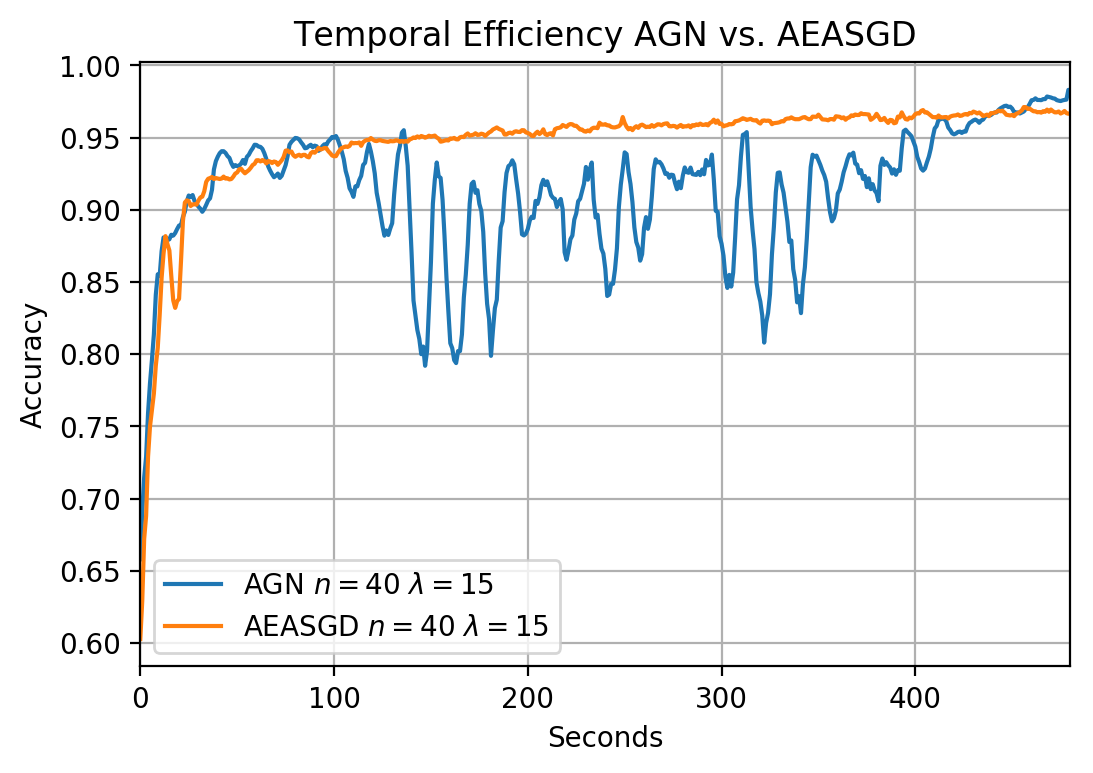
\includegraphics[width=\linewidth]{resources/images/agn_aeasgd_temporal_worst}
    \caption{$\mathcal{E}(\textsc{agn}, \textsc{aeasgd}) = 0.964$}
  \end{subfigure}
  \begin{subfigure}{.3\textwidth}
    \centering
    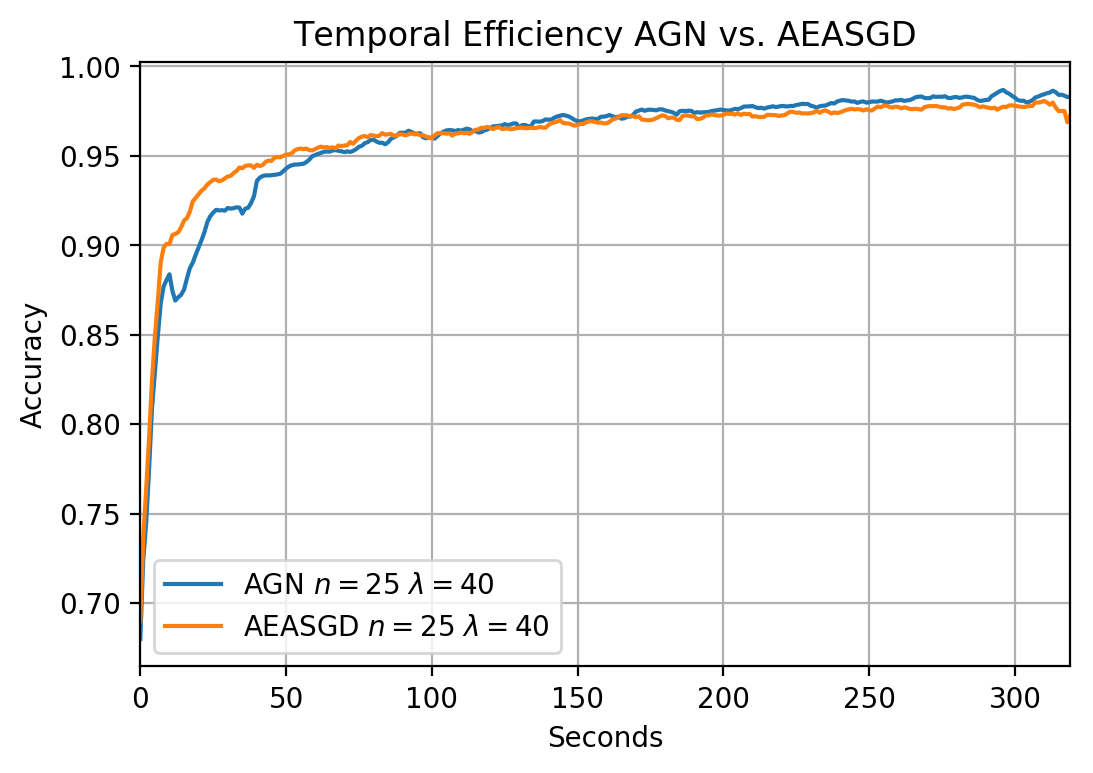
\includegraphics[width=\linewidth]{resources/images/agn_aeasgd_temporal_equal}
    \caption{$\mathcal{E}(\textsc{agn}, \textsc{aeasgd}) = 0.999$}
  \end{subfigure}
  \begin{subfigure}{.3\textwidth}
    \centering
    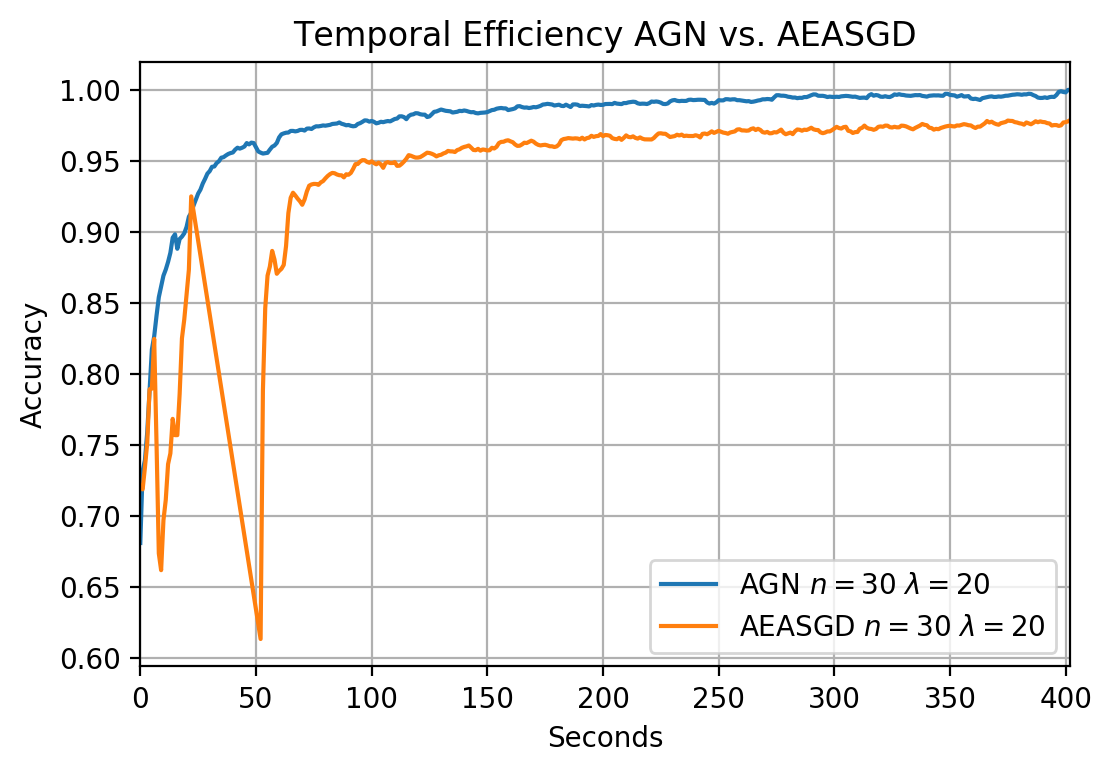
\includegraphics[width=\linewidth]{resources/images/agn_aeasgd_temporal_best}
    \caption{$\mathcal{E}(\textsc{agn}, \textsc{aeasgd}) = 1.044$}
  \end{subfigure}
  \caption{Several accuracy plots of \textsc{agn} and \textsc{aeasgd}. All subfigures show the computed \emph{temporal efficiency} of \textsc{agn}, which were obtained by applying Equation~\ref{eq:temporal_efficiency}.}
\end{figure}

\begin{table}
  \centering
  \begin{tabular}{|c|c|c|}
    \hline
    $n$ & $\lambda$ & Temporal Efficiency \textsc{AGN} \\
    \hline
    \hline
10 & 10 & \textbf{1.009} \\
\hline
10 & 15 & \textbf{1.012} \\
\hline
10 & 20 & \textbf{1.003} \\
\hline
10 & 25 & 0.999 \\
\hline
10 & 30 & 0.988 \\
\hline
10 & 35 & 0.990 \\
\hline
10 & 40 & 0.990 \\
\hline
15 & 10 & \textbf{1.008} \\
\hline
15 & 15 & \textbf{1.015} \\
\hline
15 & 20 & \textbf{1.009} \\
\hline
15 & 25 & \textbf{1.005} \\
\hline
15 & 30 & \textbf{1.000} \\
\hline
15 & 35 & 0.997 \\
\hline
15 & 40 & 0.994 \\
\hline
20 & 10 & 0.983 \\
\hline
20 & 15 & \textbf{1.018} \\
\hline
20 & 20 & \textbf{1.022} \\
\hline
20 & 25 & \textbf{1.009} \\
\hline
20 & 30 & \textbf{1.007} \\
\hline
20 & 35 & \textbf{1.002} \\
\hline
20 & 40 & 0.997 \\
\hline
25 & 10 & 0.954 \\
\hline
25 & 15 & \textbf{1.021} \\
\hline
25 & 20 & \textbf{1.017} \\
\hline
25 & 25 & \textbf{1.014} \\
\hline
25 & 30 & \textbf{1.008} \\
\hline
25 & 35 & \textbf{1.003} \\
\hline
25 & 40 & 0.999 \\
\hline
30 & 10 & 0.926 \\
\hline
30 & 15 & \textbf{1.017} \\
\hline
30 & 20 & \textbf{1.045} \\
\hline
30 & 25 & \textbf{1.015} \\
\hline
30 & 30 & \textbf{1.012} \\
\hline
30 & 35 & \textbf{1.005} \\
\hline
30 & 40 & \textbf{1.005} \\
\hline
35 & 10 & 0.881 \\
\hline
35 & 15 & 0.997 \\
\hline
35 & 20 & \textbf{1.017} \\
\hline
35 & 25 & \textbf{1.020} \\
\hline
35 & 30 & \textbf{1.016} \\
\hline
35 & 35 & \textbf{1.027} \\
\hline
35 & 40 & \textbf{1.012} \\
\hline
40 & 10 & \textbf{1.044} \\
\hline
40 & 15 & 0.964 \\
\hline
40 & 20 & \textbf{1.027} \\
\hline
40 & 25 & \textbf{1.025} \\
\hline
40 & 30 & 0.997 \\
\hline
40 & 35 & \textbf{1.009} \\
\hline
40 & 40 & \textbf{1.009} \\
\hline
  \end{tabular}
  \caption{Temporal efficiency of \textsc{agn} and \textsc{aeasgd} compared to different distributed hyperparameters. Using this information, we can deduce that \textsc{agn} is outperforming \textsc{aeasgd} in 69.73\% of the cases, which is significantly better. Furthermore, this statistic includes cases which are known where \textsc{agn} is performing worse, i.e., small amount of asynchrony, low communication frequency, and high amount of asynchrony, and high communication frequency.}
  \label{table:agn_temporal_efficiency}
\end{table}

\begin{table}
  \centering
  \begin{tabular}{|c|c|c|c|c|c|c|c|}
    \hline
    $n$ & $\lambda$ & \textsc{AGN} $t$ & \textsc{AGN} Acc. & \textsc{AGN} Val. & \textsc{AEASGD} $t$ & \textsc{AEASGD} Acc. & \textsc{AEASGD} Val. \\
    \hline
    \hline
10 & 10 & 1066.08s & \textbf{100.00\%} & 98.43\% & \textbf{953.61s} & 99.22\% & \textbf{98.64\%}  \\
\hline
10 & 15 & 864.01s & \textbf{99.53\%} & 98.54\% & \textbf{846.86s} & 99.38\% & \textbf{98.69\%}  \\
\hline
10 & 20 & 886.34s & \textbf{99.38\%} & 98.61\% & \textbf{804.07s} & 98.91\% & \textbf{98.67\%}  \\
\hline
10 & 25 & 855.51s & 98.75\% & 98.52\% & \textbf{784.46s} & \textbf{98.91\%} & \textbf{98.74\%}  \\
\hline
10 & 30 & \textbf{886.01s} & \textbf{99.22\%} & 98.50\% & 930.73s & 98.91\% & \textbf{98.64\%}  \\
\hline
10 & 35 & 850.87s & 98.44\% & 98.42\% & \textbf{798.74s} & \textbf{99.22\%} & \textbf{98.62\%}  \\
\hline
10 & 40 & 845.21s & \textbf{98.75\%} & 98.43\% & \textbf{791.04s} & 97.66\% & \textbf{98.58\%}  \\
\hline
15 & 10 & 979.72s & \textbf{99.67\%} & 98.61\% & \textbf{813.32s} & 99.11\% & \textbf{98.67\%}  \\
\hline
15 & 15 & \textbf{638.13s} & \textbf{99.89\%} & 98.58\% & 721.47s & 98.66\% & \textbf{98.65\%}  \\
\hline
15 & 20 & \textbf{562.72s} & \textbf{99.89\%} & 98.49\% & 564.92s & 99.00\% & \textbf{98.60\%}  \\
\hline
15 & 25 & 580.71s & \textbf{98.77\%} & 98.50\% & \textbf{542.28s} & 98.33\% & \textbf{98.62\%}  \\
\hline
15 & 30 & \textbf{544.97s} & 98.44\% & 98.44\% & 660.58s & \textbf{98.55\%} & \textbf{98.58\%}  \\
\hline
15 & 35 & \textbf{562.93s} & \textbf{98.66\%} & 98.45\% & 573.54s & 98.33\% & 98.45\%  \\
\hline
15 & 40 & \textbf{561.17s} & \textbf{99.22\%} & 98.42\% & 566.00s & 98.88\% & \textbf{98.52\%}  \\
\hline
20 & 10 & 839.94s & \textbf{99.26\%} & 98.36\% & \textbf{821.12s} & 97.90\% & \textbf{98.52\%}  \\
\hline
20 & 15 & \textbf{571.17s} & \textbf{100.00\%} & 98.45\% & 610.88s & 98.52\% & \textbf{98.49\%}  \\
\hline
20 & 20 & \textbf{432.93s} & \textbf{99.38\%} & \textbf{98.47\%} & 510.72s & 97.78\% & 98.39\%  \\
\hline
20 & 25 & 479.72s & \textbf{99.63\%} & \textbf{98.45\%} & \textbf{421.50s} & 97.86\% & 98.34\%  \\
\hline
20 & 30 & 433.36s & \textbf{99.42\%} & \textbf{98.49\%} & \textbf{429.16s} & 98.36\% & 98.33\%  \\
\hline
20 & 35 & 418.83s & \textbf{98.52\%} & \textbf{98.44\%} & \textbf{409.86s} & 98.19\% & 98.33\%  \\
\hline
20 & 40 & 434.86s & \textbf{98.44\%} & \textbf{98.34\%} & \textbf{420.46s} & 97.66\% & 98.28\%  \\
\hline
25 & 10 & 768.45s & \textbf{98.62\%} & 97.87\% & \textbf{753.27s} & 98.26\% & \textbf{98.40\%}  \\
\hline
25 & 15 & \textbf{524.85s} & \textbf{99.76\%} & \textbf{98.57\%} & 540.20s & 98.32\% & 98.32\%  \\
\hline
25 & 20 & 455.92s & \textbf{99.70\%} & \textbf{98.52\%} & \textbf{401.17s} & 97.66\% & 98.23\%  \\
\hline
25 & 25 & \textbf{351.30s} & \textbf{99.10\%} & \textbf{98.44\%} & 372.74s & 98.44\% & 98.26\%  \\
\hline
25 & 30 & 365.58s & \textbf{98.56\%} & \textbf{98.48\%} & \textbf{364.29s} & 98.20\% & 98.14\%  \\
\hline
25 & 35 & \textbf{364.04s} & \textbf{98.32\%} & \textbf{98.46\%} & 371.01s & 97.54\% & 98.02\%  \\
\hline
25 & 40 & 373.22s & \textbf{98.05\%} & \textbf{98.35\%} & \textbf{346.99s} & 97.72\% & 98.04\%  \\
\hline
30 & 10 & 778.42s & 97.92\% & 97.25\% & \textbf{764.59s} & \textbf{99.17\%} & \textbf{98.28\%}  \\
\hline
30 & 15 & \textbf{507.43s} & \textbf{99.72\%} & \textbf{98.51\%} & 527.42s & 98.12\% & 98.13\%  \\
\hline
30 & 20 & \textbf{428.09s} & \textbf{99.74\%} & \textbf{98.48\%} & 461.58s & 97.92\% & 98.03\%  \\
\hline
30 & 25 & 341.44s & \textbf{99.01\%} & \textbf{98.48\%} & \textbf{334.52s} & 98.59\% & 97.96\%  \\
\hline
30 & 30 & 318.41s & \textbf{99.17\%} & \textbf{98.39\%} & \textbf{310.19s} & 97.66\% & 97.77\%  \\
\hline
30 & 35 & 312.96s & \textbf{99.17\%} & \textbf{98.35\%} & \textbf{305.48s} & 98.28\% & 97.86\%  \\
\hline
30 & 40 & \textbf{316.68s} & \textbf{98.65\%} & \textbf{98.30\%} & 343.07s & 98.28\% & 97.73\%  \\
\hline
35 & 10 & \textbf{691.38s} & 96.65\% & 96.74\% & 785.00s & \textbf{98.09\%} & \textbf{97.96\%}  \\
\hline
35 & 15 & \textbf{511.17s} & \textbf{99.01\%} & \textbf{98.18\%} & 515.88s & 97.91\% & 98.06\%  \\
\hline
35 & 20 & \textbf{390.05s} & \textbf{99.61\%} & \textbf{98.51\%} & 405.90s & 97.77\% & 98.01\%  \\
\hline
35 & 25 & \textbf{314.71s} & \textbf{99.52\%} & \textbf{98.37\%} & 324.66s & 97.82\% & 97.81\%  \\
\hline
35 & 30 & \textbf{273.62s} & \textbf{98.67\%} & \textbf{98.43\%} & 379.93s & 97.63\% & 97.82\%  \\
\hline
35 & 35 & \textbf{276.11s} & \textbf{99.29\%} & \textbf{98.13\%} & 357.71s & 97.50\% & 97.84\%  \\
\hline
35 & 40 & \textbf{284.50s} & \textbf{98.69\%} & \textbf{98.17\%} & 543.86s & 97.79\% & 97.59\%  \\
\hline
40 & 10 & \textbf{748.94s} & 94.17\% & 95.55\% & 1256.09s & \textbf{96.57\%} & \textbf{97.99\%}  \\
\hline
40 & 15 & \textbf{506.25s} & 95.99\% & 97.25\% & 534.42s & \textbf{96.88\%} & \textbf{97.89\%}  \\
\hline
40 & 20 & \textbf{383.51s} & \textbf{99.24\%} & \textbf{98.40\%} & 412.37s & 96.65\% & 97.83\%  \\
\hline
40 & 25 & \textbf{308.15s} & \textbf{98.86\%} & \textbf{98.39\%} & 347.50s & 96.65\% & 97.67\%  \\
\hline
40 & 30 & 351.54s & \textbf{98.66\%} & \textbf{98.45\%} & \textbf{305.50s} & 96.47\% & 97.67\%  \\
\hline
40 & 35 & 279.30s & \textbf{98.73\%} & \textbf{98.32\%} & \textbf{252.70s} & 96.32\% & 97.60\%  \\
\hline
40 & 40 & 257.62s & \textbf{97.88\%} & \textbf{98.18\%} & \textbf{250.74s} & 96.65\% & 97.45\%  \\
\hline
  \end{tabular}
  \caption{Summary of \textsc{agn} and \textsc{aeasgd} experiments using different distributed hyperparameters ($n$ and $\lambda$). From these experiments we find that \textsc{agn} performs better in terms of training, and validation accuracy in the precense of a higher number of asynchronous workers, and a reduced communication frequency.}
  \label{table:agn_experiments_summary}
\end{table}

\begin{figure}
  \centering
  \begin{subfigure}{.3\textwidth}
    \centering
    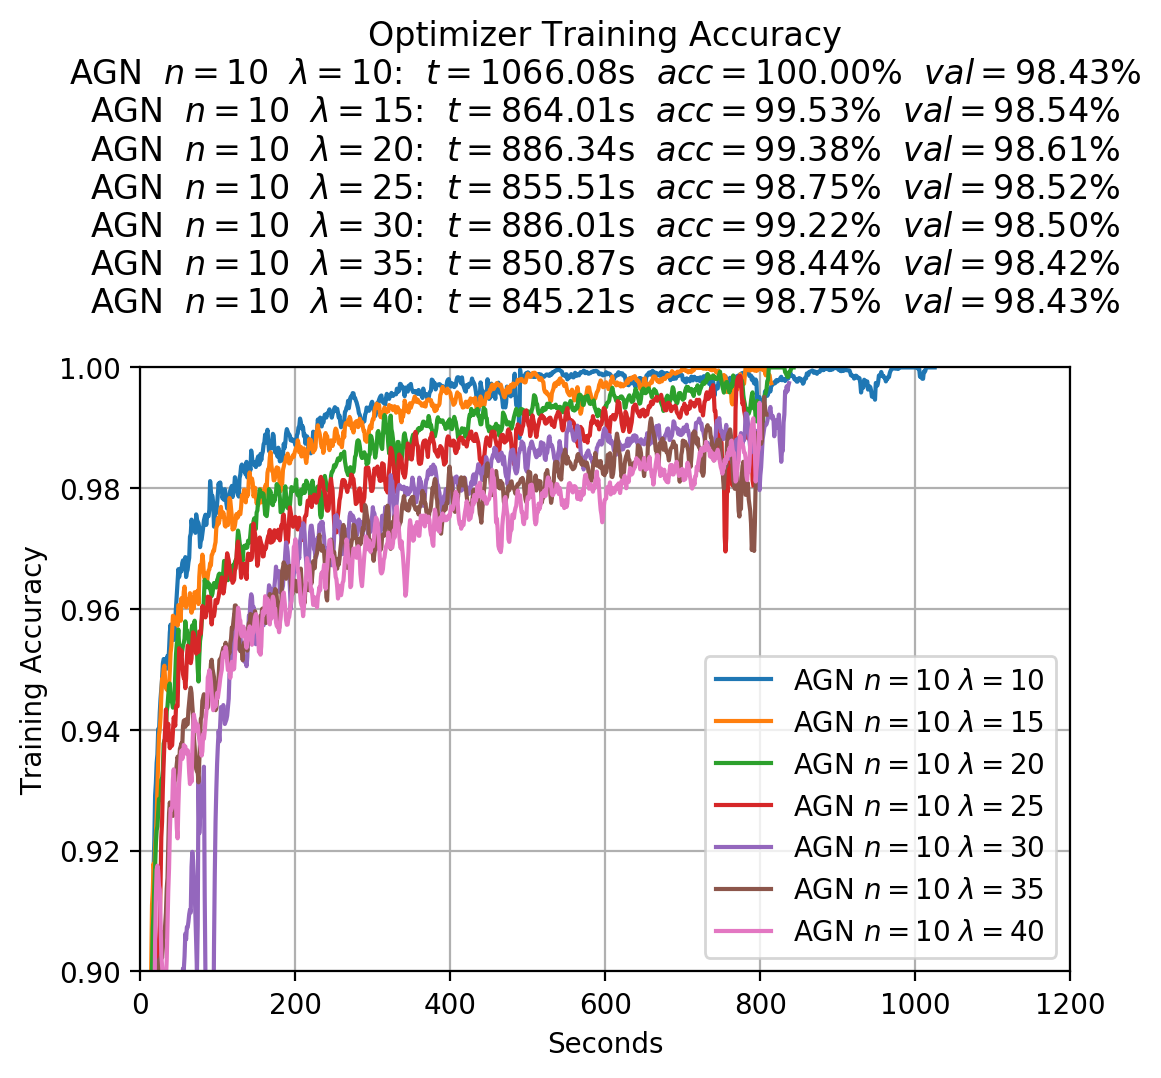
\includegraphics[width=\linewidth]{resources/images/agn_experiments_workers_10}
    \caption{$n = 10$}
  \end{subfigure}
  \begin{subfigure}{.3\textwidth}
    \centering
    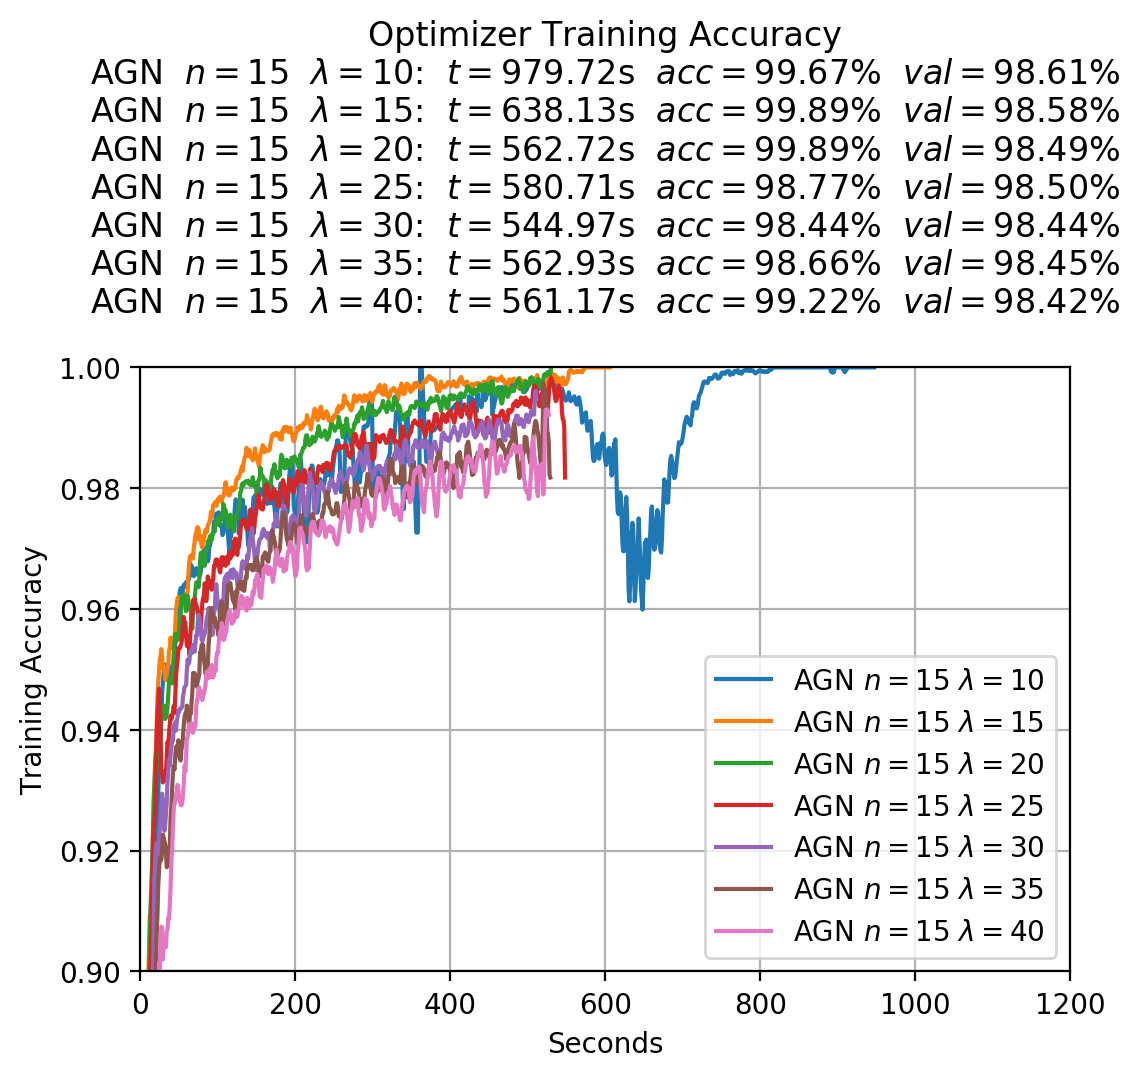
\includegraphics[width=\linewidth]{resources/images/agn_experiments_workers_15}
    \caption{$n = 15$}
  \end{subfigure}
  \begin{subfigure}{.3\textwidth}
    \centering
    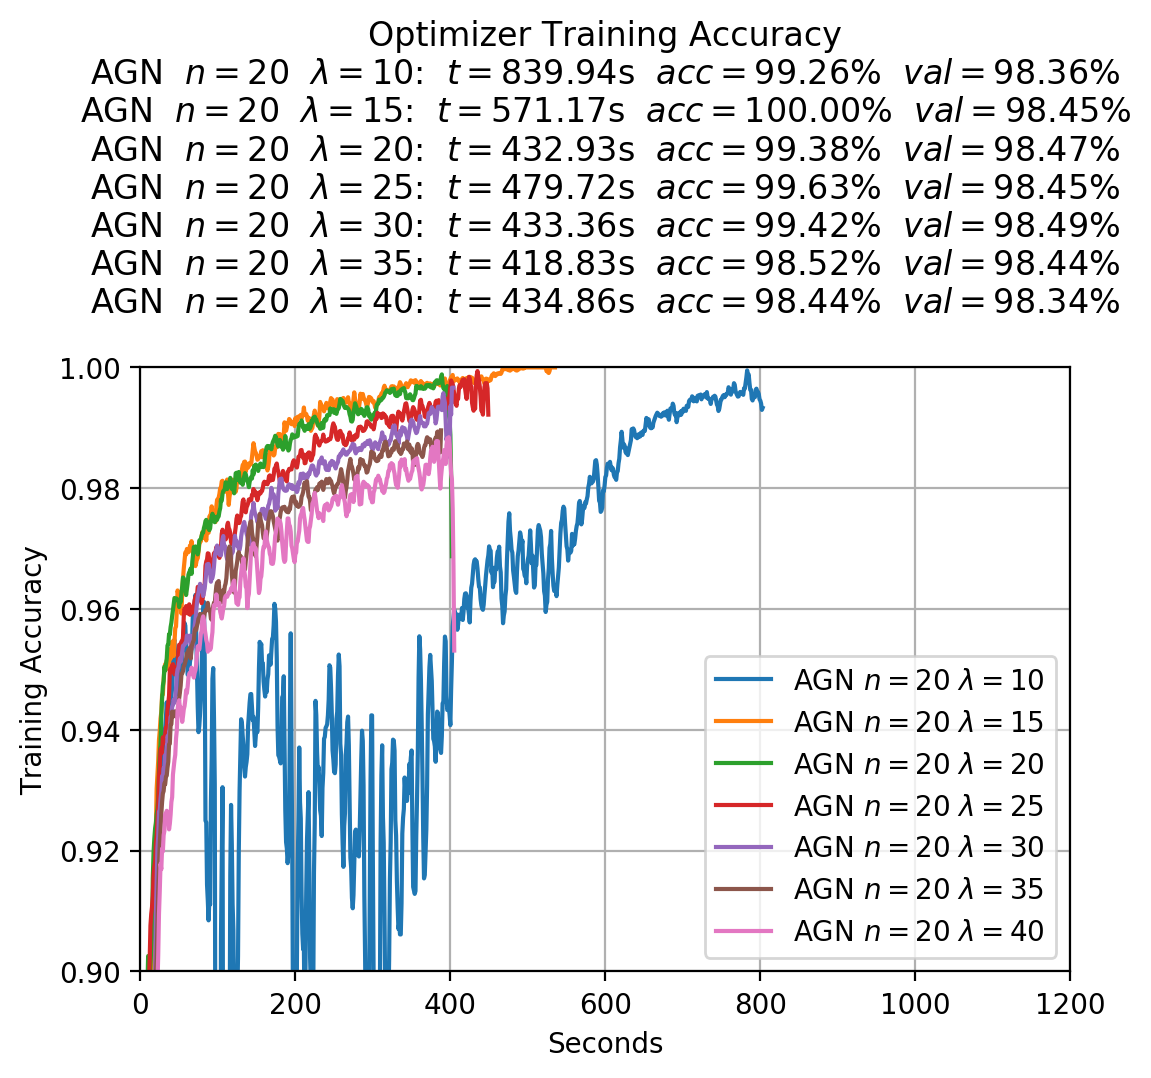
\includegraphics[width=\linewidth]{resources/images/agn_experiments_workers_20}
    \caption{$n = 20$}
  \end{subfigure}
  \begin{subfigure}{.3\textwidth}
    \centering
    \includegraphics[width=\linewidth]{resources/images/agn_experiments_workers_25}
    \caption{$n = 25$}
  \end{subfigure}
  \begin{subfigure}{.3\textwidth}
    \centering
    \includegraphics[width=\linewidth]{resources/images/agn_experiments_workers_30}
    \caption{$n = 30$}
  \end{subfigure}
  \begin{subfigure}{.3\textwidth}
    \centering
    \includegraphics[width=\linewidth]{resources/images/agn_experiments_workers_35}
    \caption{$n = 35$}
  \end{subfigure}
  \begin{subfigure}{.3\textwidth}
    \centering
    \includegraphics[width=\linewidth]{resources/images/agn_experiments_workers_40}
    \caption{$n = 40$}
  \end{subfigure}
  \caption{This Figure shows several experiments were we fixed the number of workers, but vary the communication frequency. From this we observe that \textsc{agn} performs well when a relatively equal high communication frequency is used with respect to the number of workers, and derrive the following heuristic $\lambda \approx \frac{n + \text{layers in network}}{2}$. Furthermore, increasing the amount of workers, and maintaining a high communication frequency deteriorates the performance of the central variable as well. As a result, a balance between the communication frequency, and the number of asynchronous workers is required.}
  \label{fig:agn_experiments_workers}
\end{figure}

\begin{figure}
  \centering
  \begin{subfigure}{.3\textwidth}
    \centering
    \includegraphics[width=\linewidth]{resources/images/agn_experiments_lambda_10}
    \caption{$\lambda = 10$}
  \end{subfigure}
  \begin{subfigure}{.3\textwidth}
    \centering
    \includegraphics[width=\linewidth]{resources/images/agn_experiments_lambda_15}
    \caption{$\lambda = 15$}
  \end{subfigure}
  \begin{subfigure}{.3\textwidth}
    \centering
    \includegraphics[width=\linewidth]{resources/images/agn_experiments_lambda_20}
    \caption{$\lambda = 20$}
  \end{subfigure}
  \begin{subfigure}{.3\textwidth}
    \centering
    \includegraphics[width=\linewidth]{resources/images/agn_experiments_lambda_25}
    \caption{$\lambda = 25$}
  \end{subfigure}
  \begin{subfigure}{.3\textwidth}
    \centering
    \includegraphics[width=\linewidth]{resources/images/agn_experiments_lambda_30}
    \caption{$\lambda = 30$}
  \end{subfigure}
  \begin{subfigure}{.3\textwidth}
    \centering
    \includegraphics[width=\linewidth]{resources/images/agn_experiments_lambda_35}
    \caption{$\lambda = 35$}
  \end{subfigure}
  \begin{subfigure}{.3\textwidth}
    \centering
    \includegraphics[width=\linewidth]{resources/images/agn_experiments_lambda_40}
    \caption{$\lambda = 40$}
  \end{subfigure}
  \caption{In this experiment we clamp the communication frequency, but vary the number of asynchronous workers. Due to the equal communication frequency, we can observe good scaling properties of \textsc{agn}. In most cases doubling the number of workers, reducing the training time by half and is more temporally efficient. However, for larger number of workers $n > 30$ we do not observe a reduction of training time. This is due to the implementation of our parameter server, which is based on Python threads instead of Python processes, as will be dicussed in Chapter~\ref{chapter:experiments}. Furthermore, note that reducing the amount of computational resources might actually benifit the training accuracy of the central variable, as a smaller number of asynchronous workers reduces the amount of staleness that can be incorperated in the central variable.}
  \label{fig:agn_experiments_lambdas}
\end{figure}

\begin{figure}
  \centering
  \begin{subfigure}{.3\textwidth}
    \centering
    \includegraphics[width=\linewidth]{resources/images/aeasgd_experiments_workers_10}
    \caption{$n = 10$}
  \end{subfigure}
  \begin{subfigure}{.3\textwidth}
    \centering
    \includegraphics[width=\linewidth]{resources/images/aeasgd_experiments_workers_15}
    \caption{$n = 15$}
  \end{subfigure}
  \begin{subfigure}{.3\textwidth}
    \centering
    \includegraphics[width=\linewidth]{resources/images/aeasgd_experiments_workers_20}
    \caption{$n = 20$}
  \end{subfigure}
  \begin{subfigure}{.3\textwidth}
    \centering
    \includegraphics[width=\linewidth]{resources/images/aeasgd_experiments_workers_25}
    \caption{$n = 25$}
  \end{subfigure}
  \begin{subfigure}{.3\textwidth}
    \centering
    \includegraphics[width=\linewidth]{resources/images/aeasgd_experiments_workers_30}
    \caption{$n = 30$}
  \end{subfigure}
  \begin{subfigure}{.3\textwidth}
    \centering
    \includegraphics[width=\linewidth]{resources/images/aeasgd_experiments_workers_35}
    \caption{$n = 35$}
  \end{subfigure}
  \begin{subfigure}{.3\textwidth}
    \centering
    \includegraphics[width=\linewidth]{resources/images/aeasgd_experiments_workers_40}
    \caption{$n = 40$}
  \end{subfigure}
  \caption{\textsc{aeasgd} fixed worker, with varying communication frequency experiments. As suggested by the author, \textsc{aeasgd} usually benifits from an increased amount of local worker (large $\lambda$). Furthermore, we observe that initially, \textsc{aeasgd} is quite robust to hyperparameterization ($n = 10$). However, as the number of asynchronous workers increases, and the communication frequency is further reduced, the accuracy plots start to deviate to the point that they \emph{flatten} at a suboptimal training accuracy. Meaning, a lower training accuracy compared to other configurations, where \textsc{aeasgd} reached a significantly higher training accuracy.}
  \label{fig:aeasgd_experiments_workers}
\end{figure}

\begin{figure}
  \centering
  \begin{subfigure}{.3\textwidth}
    \centering
    \includegraphics[width=\linewidth]{resources/images/aeasgd_experiments_lambda_10}
    \caption{$\lambda = 10$}
  \end{subfigure}
  \begin{subfigure}{.3\textwidth}
    \centering
    \includegraphics[width=\linewidth]{resources/images/aeasgd_experiments_lambda_15}
    \caption{$\lambda = 15$}
  \end{subfigure}
  \begin{subfigure}{.3\textwidth}
    \centering
    \includegraphics[width=\linewidth]{resources/images/aeasgd_experiments_lambda_20}
    \caption{$\lambda = 20$}
  \end{subfigure}
  \begin{subfigure}{.3\textwidth}
    \centering
    \includegraphics[width=\linewidth]{resources/images/aeasgd_experiments_lambda_25}
    \caption{$\lambda = 25$}
  \end{subfigure}
  \begin{subfigure}{.3\textwidth}
    \centering
    \includegraphics[width=\linewidth]{resources/images/aeasgd_experiments_lambda_30}
    \caption{$\lambda = 30$}
  \end{subfigure}
  \begin{subfigure}{.3\textwidth}
    \centering
    \includegraphics[width=\linewidth]{resources/images/aeasgd_experiments_lambda_35}
    \caption{$\lambda = 35$}
  \end{subfigure}
  \begin{subfigure}{.3\textwidth}
    \centering
    \includegraphics[width=\linewidth]{resources/images/aeasgd_experiments_lambda_40}
    \caption{$\lambda = 40$}
  \end{subfigure}
  \caption{In this experiment we clamp the communication frequency, but vary the number of workers. As in Figure~\ref{fig:aeasgd_experiments_workers}, we do similar observations regarding the flattening of the training accuracy in the precense of a low communication frequency, and a large amount of asynchrony. However, an additional interesting observation which escaped our eye in Figure~\ref{fig:aeasgd_experiments_workers}, is the large ``bump'' in training accuracy for $n = 10$. Nevertheless, this bump is always followed up by a significant reduction in training accuracy. Usually one would expect such behaviour in a configuration with a large amount of asynchrony, but this behaviour is not present is said configurations. Furthermore, the reason why we do not observe significant fluctuations in training accuracy, contrary to \textsc{agn}, is due to hyperparameter $\rho$, which controls the amount of exploration that can be done in terms of \emph{distance}, as discussed in Chapter~\ref{chapter:distributed_deep_learning}.}
  \label{fig:aeasgd_experiments_lambdas}
\end{figure}

% Chapter on Asynchronous Distributed Adaptive Gradient
%
% Developed for my Master Thesis at Maastricht University.
% Based on Eugenio Senes's template at the University of Torino.
%
% By Joeri Hermans (joeri@joerihermans.com)
%
% Released under an MIT license. Share, modify and enjoy, but quote the author!

\chapter{Asynchronous Distributed Adaptive Gradients}
\label{chapter:asynchronous_distributed_adaptive_gradients}

In this chapter we introduce a novel optimizer called \textsc{adag}. \textsc{adag}, or \emph{Asynchronous Distributed Adaptive Gradients}, is an optimization process designed with data parallel methods in mind. We build upon previous work~\cite{dean2012large,hadjis2016omnivore,kingma2014adam,zhang2015deep,jiang2017heterogeneity} and incorperate new insights backed up by theory and experimental evidence. We start in Section~\ref{sec:adag_problem_setting} by formalizing the problem setting. Section~\ref{sec:adag_algorithm} describes our algorithm in detail, supported by intuition and theory. Finally, we experimentally show the effectiveness of our approach in Section~\ref{sec:adag_experiments} and give some points for future work in Section~\ref{sec:adag_future_work}.

\section{Problem setting}
\label{sec:adag_problem_setting}

Currently, staleness $\tau$ is defined in literature as the number of steps between the current timestep $t$ of the central variable, and the timestep of the central variable which a worker based its gradients upon, which is $t - \tau$. However, as shown in Chapter~\ref{chapter:distributed_deep_learning} and Chapter~\ref{chapter:accumulated_gradient_normalization}, this particular definition of staleness is problematic when one tries to mitigate parameter staleness. To illustrate this, we showed in Chapter~\ref{chapter:accumulated_gradient_normalization} that \textsc{dynsgd}~\cite{jiang2017heterogeneity}, which uses the above definition of staleness, is not able to solve the staleness problem if the learning rate is too high or gradient accumulation takes place, i.e., if the magnitude of the worker deltas is too large. Since \textsc{dynsgd} fails to deal with staleness efficiently in those situations, one can deduce that using the number of stale steps is a rather naive approach. As a result, the problem of parameter staleness in Deep Learning has an additional dimension.\\

A step forward in understanding the staleness problem is by gaining intuition on what mechanism is exactly causing the central variable to diverge, or converge more slowly. As mentioned in Chapter~\ref{chapter:introduction}, divergent behaviour of the central variable is caused by stale workers committing gradients which are based on old parameterizations of the central variable. Again, in this definition we use the term ``old''. However, we argue in the following sections that an old central variable is not problematic as long as the \emph{distance} between the old, and the current central variable is small. To strengthen this intuition, let us consider Figure~\ref{fig:async_momentum} from Chapter~\ref{fig:async_momentum}. Clearly, the reason why the central variable diverges is because the straggler commits a gradient which was based on a completely different loss (position). Hypothetically, let us consider that only a single other worker committed a gradient causing the central variable to be close to a minima. If one would employ an optimizer like \textsc{dynsgd}, which uses a definition of staleness based on the number of stale \emph{steps}, the stale gradient would be scaled down by half, causing significant divergent behaviour in the central variable. However, if one would use the \emph{distance} between the current, and the old central variable, and scale the workers deltas proportionally to this distance, one is able to simply ignore the result of the straggler thus preventing divergent behaviour. This intuition is shown in Figure~\ref{fig:adag_straggler_corrected}, which incorperates the delta from the straggler into the central variable using Equation~\ref{eq:adag}.\\

\begin{figure}[H]
  \centering
  \includegraphics[width=\textwidth]{resources/images/async_straggler_corrected_adag}
  \caption{Correction of the stale worker delta using Equation~\ref{eq:adag}. Contrary to Figure~\ref{fig:async_momentum}, the gradient is scaled down significantly in a way it does not deteriorate the performance of the central variable.}
  \label{fig:adag_straggler_corrected}
\end{figure}

An interesting observation from Chapter~\ref{chapter:accumulated_gradient_normalization}, is that contrary to \textsc{agn}, \textsc{aeasgd} does not show any divergent behaviour for most configurations, i.e., in terms of distributed hyperparameterizations. This is rather interesting, because it tells us that \textsc{aeasgd} has an intrinsic mechanism to deal with parameter staleness. If we review Equation~\ref{eq:aeasgd_worker}, which describes the worker update rule for $\lambda = 1$, we see the that the elastic difference, defined as $\eta_t\rho(\theta^k_t - \tilde{\theta}_t)$, incorperates the \emph{distance} between the worker parameterization $\theta^k_t$ and the \emph{current} parameterization of the central variable $\tilde{\theta}_t$. \textsc{aeasgd} uses the elastic difference as an \emph{opposing force} of the worker exploration, meaning, it limits the amount of exploration that can be done. As a result, the elastic difference of \textsc{aeasgd} in effect limits the \emph{distance} that can be covered by the worker (unless the gradients suddenly become larger). As a result, \textsc{aeasgd} serves as additional evidence for our notion that staleness should be defined in terms of \emph{distance}, and not in terms of stale steps, as formalized in Defination~\ref{def:staleness}.

\begin{definition}{Staleness}
  \label{def:staleness}
  Given a parameterization for worker $k$ at time $t$, $\theta^k_t$, based on the central variable $\tilde{\theta}_{t - \tau}$ where $\tau$ is the number of stale steps, and a central variable at time $t$, $\tilde{\theta}_t$. Then, staleness is defined as the difference (distance) between $\tilde{\theta}_t$ and $\tilde{\theta}_{t-\tau}$.
\end{definition}

Using Definition~\ref{def:staleness}, we can make the deduction that staleness is not really a problem as long as workers commit gradients based on older parameterization of the central variable, which are close to the \emph{current} central variable. This is again additional support for Hypothesis~\ref{hyp:local_optimization}, which states that workers only contribute efficiently to the central variable as they remain close to each other, i.e., the variance of the workers amount the parameter space is small.

\section{Algorithm \& Update Rule}
\label{sec:adag_algorithm}

This Section fully describes the \textsc{adag} update rule, and several architectural decisions that can be made when implementing this technique. Furthermore, using Definition~\ref{def:staleness}, we show how \textsc{adag} can push the limits of asynchronous optimization further, while at the same time eliminating the need for (distributed) hyperparameter gridsearches to ensure convergence.\\

To describe the \textsc{adag} update rule, we use the same terminology and notation used in Definition~\ref{def:staleness} to further strengthen the intuition in parameter staleness, and how parameter staleness is used in Equation~\ref{eq:adag}. Let us consider the case when $\tau = 0$. In this situation, a worker $k$ computes the gradient based on $\tilde{\theta}_{t-\tau}$ which is equal to $\tilde{\theta}_t$. As a result, the distance between these two parameterizations will be 0, which results in the worker delta $\Delta\theta^k$ to be incorperated into the central variable \emph{as is}, and thereby causing the \textsc{adag} update rule to generalize to \textsc{sgd}. In the next step, we add more asynchronous workers to the optimization problem. By doing so, we implicitly increase the staleness as $\mathbf{E}[\tau] = (n - 1)$. As a result, parameter staleness in terms of stale steps, $\tau$, is expected to be larger than 0. Consequently, the distance between $\tilde{\theta}_t$ and $\tilde{\theta}_{t - \tau}$ is \emph{expected} to be non-zero causing the worker delta to be scaled down proportionally to the difference of these parameterizations. However, since parameter changes in Deep Learning usually consist of very small updates, we use the inverse learning rate ($\eta_t^{-1}$) to get a sense of the scale at which these updates operate at. Using the inverse learning rate in Equation~\ref{eq:adag}, and due to the fact that staleness (in terms of distance) is usually relatively small in Deep Learning since the gradients are scaled with respect to $\eta_t$, we find that \textsc{adag} scales the gradients more realistically. Since without the inverse learning rate, the scaling would be very small.

\begin{equation}
  \label{eq:adag}
  \tilde{\theta}_{t+1} = \tilde{\theta}_t + \ddfrac{1}{\eta_t^{-1}\|\tilde{\theta}_t - \tilde{\theta}_{t - \tau}\|^2 + 1} \odot \Delta\theta^k
\end{equation}

Nevertheless, one could view the inverse learning rate from a different perspective. Fist let us denote the set of workers as $\mathcal{W}$. Then, the staleness term in Equation~\ref{eq:adag} can be written as a sequence of gradients from different workers $w$, as shown in Equation~\ref{eq:adag_difference_1}.

\begin{equation}
  \label{eq:adag_difference_1}
  \tilde{\theta}_{t} - \tilde{\theta}_{t - \tau} = \sum_{i = 0}^\tau \exists!\, w \in \mathcal{W}: \eta_t \nabla_\theta \mathcal{L}_w(\tilde{\theta}_{t - \tau_w})
\end{equation}

Furthermore, assuming a static learning rate $\eta$, Equation~\ref{eq:adag_difference_1} can be simplified by moving the learning rate $\eta_t$ before the summation sign, obtaining Equation~\ref{eq:adag_difference_2}.

\begin{equation}
  \label{eq:adag_difference_2}
  \tilde{\theta}_{t} - \tilde{\theta}_{t - \tau} = \eta \sum_{i = 0}^\tau \exists!\, w \in \mathcal{W}: \nabla_\theta \mathcal{L}_w(\tilde{\theta}_{t - \tau_w})
\end{equation}

Remember that the scaling of the worker deltas are proportional to Equation~\ref{eq:adag_difference_3}.

\begin{equation}
  \label{eq:adag_difference_3}
  \eta^{-1} \|\tilde{\theta}_t - \tilde{\theta}_{t - \tau}\|^2
\end{equation}

Substituting the staleness term in Equation~\ref{eq:adag_difference_3} for Equation~\ref{eq:adag_difference_2} gives us:

\begin{equation}
  \label{eq:adag_difference_4}
  \eta^{-1}\|\eta\sum_{i = 0}^\tau \exists!\, w \in \mathcal{W}: \nabla_\theta \mathcal{L}_w(\tilde{\theta}_{t - \tau_w})\|^2
\end{equation}

Earlier, the assumption was made the learning rate is static. As a result, we can cancel the learning rate terms, and thus obtaining Equation~\ref{eq:adag_difference_5}.

\begin{equation}
  \label{eq:adag_difference_5}
  \cancel{\eta^{-1}}\|\cancel{\eta}\sum_{i = 0}^\tau \exists!\, w \in \mathcal{W}: \nabla_\theta \mathcal{L}_w(\tilde{\theta}_{t - \tau_w})\|^2
\end{equation}

This result indicates that the scaling term in Equation~\ref{eq:adag} is proportional to a \emph{unitless} sequence of worker gradients, i.e., not scaled down by a learning rate. As a result, Equation~\ref{eq:adag} is not sensitive to the hyperparameterization of $\eta$. Therefore, the scaling term will work at any scale, and still be proportional to the magnitude of the worker gradients.\\

An additional, but important aspect that needs to be considered is how \textsc{adag} keeps track of $\tilde{\theta}_{t - \tau}$. For this we foresee two possible implementations. The first, described in Algorithm~\ref{algo:adag_1}, keeps track of $\tilde{\theta}_{t - \tau_w}$ for a particular worker $w$ at a worker level. Meaning, worker $w$ keeps track of its local copy $\theta_t^w$, and the original central variable $\tilde{\theta}_{t-\tau}$. Next, when worker $w$ is done computing $\Delta\theta^w_t$, $w$ will commit both $\Delta\theta^w_t$ and $\tilde{\theta}_{t - \tau}$ to the parameter server. Since the parameter server already holds $\tilde{\theta}_{t}$, the parameter server can now compute the next central variable using Equation~\ref{eq:adag}.

\begin{algorithm}[H]
  \caption{Implementation of \textsc{adag} where the workers are responsible for keeping track of $\tilde{\theta}_{t - \tau}$.}
  \label{algo:adag_1}
  \begin{algorithmic}[1]
    \Procedure{ADAGParameterServer}{}
    \State $t \gets 0$ \Comment{Parameter server clock}
    \State $\tilde{\theta}_t \gets \Call{Random}$
    \State
    \Procedure{HandlePull}{$k$} \Comment{$k$ denotes the worker identifier}
    \State \Return $\tilde{\theta}_{t}$
    \EndProcedure
    \State
    \Procedure{HandleCommit}{$k$, $\Delta\theta^w$, $\tilde{\theta}_{t - \tau_k}$}
    \State $\tilde{\theta}_{t + 1} = \tilde{\theta} + \ddfrac{1}{\eta_t^{-1}\|\tilde{\theta}_t - \tilde{\theta}_{t - \tau_k}\|^2 + 1} \odot \Delta\theta^k_t$
    \State $t \gets t + 1$
    \EndProcedure
    \State
    \EndProcedure
  \end{algorithmic}
\end{algorithm}

However, an obvious limitation of Algorithm~\ref{algo:adag_1} is the increased network usage since two parameterizations have to be shipped to the parameter server, i.e., the worker delta $\Delta\theta^k_t$ and the original central variable parameterization $\tilde{\theta}_{t - \tau}$. To reduce the network usage of Algorithm~\ref{algo:adag_1}, and thereby reducing the waiting time of the workers, we propose to let the parameter server keep track of worker pulls, i.e., whenever a worker pulls the central variable, the parameter server copies the central variable into a datastructure (for example, a hashmap), and associates the the parameterization of the central variable with the worker which requested the pull at that time. This procedure is roughly described in Algorithm~\ref{algo:adag_2}. However, we would like to note that despite the fact that Algorithm~\ref{algo:adag_2} reduces the communication costs, it increases the memory requirements proportional to the number of concurrent workers. Which as a result, might be problematic as the number of asynchronous workers is high.

\begin{algorithm}[H]
  \caption{Network efficient implementation of \textsc{adag}.}
  \label{algo:adag_2}
  \begin{algorithmic}[1]
    \Procedure{ADAGParameterServer}{}
    \State $t \gets 0$ \Comment{Parameter server clock}
    \State $\tilde{\theta}_t \gets \Call{Random}$
    \State $m \gets \Call{Initialize}$ \Comment{Initializes a data structure which keeps track of worker pulls.}
    \State
    \Procedure{HandlePull}{$k$} \Comment{$k$ denotes the worker identifier}
    \State $m[k] = \tilde{\theta}_t$
    \State \Return $\tilde{\theta}_{t}$
    \EndProcedure
    \State
    \Procedure{HandleCommit}{$k$, $\Delta\theta^w$}
    \State $\tilde{\theta}_{t + 1} = \tilde{\theta} + \ddfrac{1}{\eta_t^{-1}\|\tilde{\theta}_t - m[k]\|^2 + 1} \odot \Delta\theta^k_t$
    \State $t \gets t + 1$
    \EndProcedure
    \State
    \EndProcedure
  \end{algorithmic}
\end{algorithm}

\section{Experiments}
\label{sec:adag_experiments}

To demonstrate the effectiveness of Definition~\ref{def:staleness}, several experiments shall be conducted in the following section regarding the convergence properties of \textsc{adag}. Looking back at Chapter~\ref{chapter:accumulated_gradient_normalization}, we saw that staleness mitigation is critical in highly concurrent environments, as the staleness increases proportionally to the number of workers, as shown in Figure~\ref{fig:staleness_increasing}. Furthermore, without \textsc{adag}, we have to descrease the communication frequency even further to ensure that divergence does not occur. However, as a result of the increased amount of local exploration, parameter updates occur less frequently. Which again results in a slower convergence of the central variable, and thereby reducing the \emph{temporal efficiency} of those highly concurrent configurations compared to less concurrent configurations.

\begin{figure}[H]
  \centering
  \includegraphics[width=.5\textwidth]{resources/images/plots/adag_agn_mnist/epoch_40/15/000000001/staleness_distribution}
  \caption{Staleness distribution of $n = 20$. This is in accordance with the theory~\cite{implicitmomentum}, which says that $\mathbf{E}[\tau] = (n - 1)$. Note that the $x$-axis denotes the staleness in terms of stale steps.}
  \label{fig:staleness_increasing}
\end{figure}

Let us start by considering several predictive scenarios to verify this novel understanding of parameter staleness in Deep Learning, and how to deal with it, as shown in Equation~\ref{eq:adag}. First and foremost, at the start of any parameterized machine learning training procedure, a model is initialized according to some initialization strategy. Since the probability is \emph{very} low that a randomly initialized parameterization will perform well in terms of classification accuracy, we can make the assumption that the loss during the initial phase of the training will be relatively high. Furthermore, let us assume that there are $n$ workers trying to optimize the central variable in an asynchronous manner, and that \textsc{adag} is applied before incorperating the worker deltas into the central variable, i.e., scaling proportional to $n^{-1}\|\tilde{\theta}_t - \tilde{\theta}_{t - \tau}\|^2$ is applied to the incoming worker delta. In this case, we can expect that during the initial phase of the training procedure only a few workers will contribute efficiently to the central variable. With this statement, we are implying that only the deltas of a small fraction of workers will not be scaled down significantly because the loss, and thereby the gradients are quite large at the start of the training procedure, in contrast to the situation when the central variable is close to an optimum. As a result, other workers will be scaled down significantly, because the parameterization on which they based their gradients on (which all workers started with), is too distant from the current central variable.\\

The following prediction we make is related to the convergence of optimizers which employ \textsc{adag}. First, we know that stale gradients will be scaled down significantly due to the update rule described in Equation~\ref{eq:adag}. Furthermore, since the loss is getting smaller as the training procedure goes on, staleness, in terms of Definition~\ref{def:staleness}, is implicitly getting smaller as well. As a result, if one would plot the scaling term for every worker, we should observe (on average) a decline in the scaling factor.

\begin{figure}[H]
  \centering
  % So far for file naming consistency.
  \begin{subfigure}{.3\textwidth}
    \centering
    \includegraphics[width=\linewidth]{resources/images/plots/adag_agn_mnist/epoch_40/15/001/adag_agn_scaling_overview}
    \caption{$\eta = 0.001$}
  \end{subfigure}
  \begin{subfigure}{.3\textwidth}
    \centering
    \includegraphics[width=\linewidth]{resources/images/plots/adag_agn_mnist/epoch_40/15/0001/scaling_detail}
    \caption{$\eta = 0.0001$}
  \end{subfigure}
  \begin{subfigure}{.3\textwidth}
    \centering
    \includegraphics[width=\linewidth]{resources/images/plots/adag_agn_mnist/epoch_40/15/00001/scaling_overview}
    \caption{$\eta = 0.00001$}
  \end{subfigure}
  \caption{Predictions}
  \label{fig:adag_predictions}
\end{figure}

\section{Future work}
\label{sec:adag_future_work}

% Chapter on distributed Keras.
%
% Developed for my Master Thesis at Maastricht University.
% Based on Eugenio Senes's template at the University of Torino.
%
% By Joeri Hermans (joeri@joerihermans.com)
%
% Released under an MIT license. Share, modify and enjoy, but quote the author!

\chapter{Distributed Keras}
\label{chapter:dist-keras}

% Experiments chapter.
%
% Developed for my Master Thesis at Maastricht University.
% Based on Eugenio Senes's template at the University of Torino.
%
% By Joeri Hermans (joeri@joerihermans.com)
%
% Released under an MIT license. Share, modify and enjoy, but quote the author!

\chapter{Experimental Setup}
\label{chapter:experiments}

This chapter describes the experimental setup of our experiments in Chapter~\ref{chapter:accumulated_gradient_normalization} and Chapter~\ref{chapter:asynchronous_distributed_adaptive_gradients}. Furthermore, the architecture of \emph{dist-keras}, which is our Distributed Deep Learning framework based on Apache Spark and Keras, is also introduced.

\section{Distributed Keras}
\label{sec:distributed_keras}

Distributed Keras, or \emph{dist-keras} in short, is a distributed Deep Learning framework built on top of Apache Spark and Keras with the goal to significantly reduce the training using distributed machine learning algorithms, and allow bigger than memory datasets. This project initially started as a prototype with the CMS collaboration. However, the project has seen several iterations since its start in August 2016, and is still undergoing active development~\cite{dist_keras}. Furthermore, \emph{dist-keras} is designed with a focus on "state-of-the-art" distributed optimization algorithms. We designed the framework in such a way that a new distributed optimizer could be implemented with ease, thus enabling a person to focus on research. Several distributed methods are supported, such as, but not restricted to, the training of ensembles and models using data parallel methods.

\subsection{Architecture}
\label{sec:dist_keras_architecture}

Before we dive into the architecture of \emph{dist-keras}, let us first discuss several concepts within Apache Spark, since these are heavily used in the framework. First, Apache Spark is a general purpose cluster computing framework using directed acyclic computation graphs to define a sequence of operations. This graph is constructed by a \emph{driver} program, which resposibilities are to send new instructions to worker nodes, or receive results. However, the driver program does \emph{not execute} any intructions from the DAG (directed acyclic graph). The processes which are responsible for the execution of the DAG, are called \emph{executors}. Usually, executors are spawned dynamically using a cluster resource manager. However, it is possible to spawn them manually on every cluster node with the disadvantage that job-dependent configurations (e.g., memory) are not possible.\\

Nevertheless, an additional important aspect is the way data is handled. Spark usually benefits from a large amount of memory, since it tries to fit as much as possible data in memory to increase the processing throughput. However, if the data does not fit in memory, a flag has to be specified to modify the persistance of the data, meaning, data is allowed to be serialized to disk, and read back into memory when needed. Furthermore, since a computation is defined as a DAG, data can be recomputed in the case of a potential loss due to, for example, data not fitting into memory, or serialized data not fitting on a local disk, or even an unexpected shutdown. Furthermore, to prevent a complete recomputation of data, one can \emph{cache} the data at a specific point. Basically, calling \emph{cache} (checkpointing) on a dataset, tells the executors to keep track of the data in its current form, i.e., not recomputing it. Furthermore, in order to apply modifications, or mapping functions to datasets in a distributed manner, Spark provides an abstraction of data in terms of \emph{Resilient Distributed Dataset}. As discussed before, the term \emph{resilient} implies that the data is able to recover from failures described above. Furthermore, Spark also provides some syntatic sugar in terms of DataFrames and DataSets to easily manipulate data in a tabular format. However, in contrast to regular tabular entries, data rows are not limited to a specific schema, but can be customized if desired. As a result, we can construct any particular dataset of intereset in a Spark DataFrame, and preprocess it for Deep Learning, or other analytical purposes. Furthermore, since Apache Spark provides several utilities to distribute the data among the executors, and stream the data were needed, an architecture can be constructed to feed the data to Deep Learning models in production, or during training.\\

In general, a \emph{dist-keras} workflow proceeds as follows. Initially, a Keras model is constructed on the machine were the Spark Driver will be allocated, this could be a personal laptop or desktop computer, however, it is recommended that this machine is in nearby proximity of other cluster nodes and has performant hardware including efficient networking capabilities because the parameter server will be allocated on this machine. Nevertheless, despite the fact allocating a single parameter server creates a significant bottleneck on this particular machine, especially when using large models, it proved to be sufficient for our use-cases. However, in essence it should be possible to allocate parameter servers dynamically on different machines since our current parameter server implementations does not have any Spark dependencies. Next, the data is read from a raw datasource, e.g., \emph{csv}, \emph{Apache Parquet}, or \emph{Apache Avro}, or some other data format that is supported. However, at this point the data is spread over several machines, but not all machines involved in the training procedure. To ensure fast delivery of the data to the executor, we \emph{repartiton} the data equal to the number of workers which will train the model in parallel. However, due to Spark's \emph{lazy-evaluation} mechanism, the repartitioning (shuffling) of the data is not triggered. To trigger this, we call a Spark \emph{action} such as a \emph{count}, to execute the DAG computation.

\begin{figure}[H]
  \centering
  %\includegraphics[width=.8\textwidth]{}
  \caption{dist-keras something something}
  \label{fig:dist_keras_architecture}
\end{figure}

Before starting the training procedure, all relevant objects such as model weights, optimizer, input column, output column, and so on, are serialized. After the serialization of the training configuration is done, the configuration is transported to the Spark executors, where they can be deserialized and reinstantiated. At this point, two concurrent threads will be spawned on every executor. The first thread is responsible for the prefetching of the data, since it is possibly that the data needs to be streamed from a different machine. Furthermore, this thread is also responsible for converting the prefetched training samples into the expected format, i.e., \emph{numpy matrices}. The second thread is mainly responsible for the training procedure, shown in Figure~\ref{fig:dist_keras_architecture}. This thread will implement a specific distributed optimization procedure such as \textsc{adag-agn}, \textsc{aeasgd}, or \textsc{downpour}. Nevertheless, during the training procedure, every worker will collect a set of timestamped training metrics (batch accuracy, batch loss). Meaning, after every computation of a mini-batch, the training metrics are timestamped and yielded to Spark for later processing. After all data has been processed, training metrics of all Spark executors are collected and processed to generate central variable accuracy and loss over time.\\

Finally, when the DAG computation is completed, \emph{dist-keras} fetches the most recent parameterization from the parameter server, and initializes a model with that parameterization. Afterwards, a user can potentially compute validation accuracy in a distributed manner since several utility data \emph{transformers} and \emph{predictors} are provided by \emph{dist-keras}.

\section{Use-case: CMS Event Identification}
\label{sec:experiment_track_reconstruction}

To reduce the computational load of collision reconstructions in future LHC runs, the CMS experiment is exploring Machine Learning techniques as a possible approach for accomplishing this. In this particular case, the experiment is evaluating Deep Learning techniques by fitting them to physics problems. High-level problems such as deciding which data to keep in the High Level Trigger given some physical attributes, and other inference problems, are possible applications. Not because of a statistical perspective perce, but mostly to reduce computational complexity. In the following experiments, we mainly occupy ourselves with the reconstruction of \emph{particle tracks}, and identification of \emph{track types} from raw detector \emph{hits}. A particle track, \emph{track} denoted from this point on, is the path that has been traversed by a particle through the detector. The track is reconstructed from a set of hits, which have been triggered (detected) by parts of the detector. The reconstruction of these tracks is a computationally intensive process, since given a set of hits, one needs to minimize the $\chi^2$ error of the track with respect to the set of hits that have been associated with a particular track. However, this is only one aspect of the problem, one first needs to obtain the set of hits which describe a track given all hits within a collision, which also includes the background (false-positives) generated by the detector itself. Currently, the set of hits related to a single track are extracted using a two-pass Kalman filter and a iterative method to find the best fit, with the first pass of the Kalman filter starting on the outer edges of the detector.\\

An additional problem of applying Deep Learning, or any other Machine Learning approach to the problem of track reconstruction, or event identification, is the petabyte scale data that needs to be dealth with. A simple, and more common solution would be to sample a more managable fraction of the dataset to train our models on. However, we want the model to be able to extract as many diverse tracks as possible that have been reconstructed over previous years by reconstruction software. As a result, a distributed (data parallel) approach is necessary. However, the data representation is also an important aspect of the problem. Currently, all collisions are stored in the \textsc{root} format, where every reconstructed track for a particular collision (or set of collisions), including the hits of the track, and track parameters can be extracted from. This specific data format is quite problematic, especially taking the petabyte-scale data into account. Furthermore, depending on the modelling, the data needs to be preprocessed in a particular way. One could of course preprocess the complete physics data in a format, shape the data accordingly, and simply copy the data to the machines which will be used during training. However, this is not a very space efficient approach.\\

A more reasonable, and space efficient approach would be to deliver the preprocessed data to the training procedure in a streaming manner. For example, every worker has a buffer in which it will prefetch and preprocess data coming from the \textsc{root} format in a way the model will understand, e.g., \emph{numpy} arrays. This approach does not have the space inefficiencies the previous approach had. However, there is an increased computational load on the worker nodes due to the prefetching, preprocessing of the data, and duplicate processing of the same training samples if multiple epochs of training are required. Nevertheless, compared to computation of gradients in large models, this load is neglectable. An additional benefit of this approach is that the same architecture can be used during model development, since data representations can be generated on-the-fly as in Apache Spark, shown in Figure~\ref{fig:experiment_cms_tracking}.

\begin{figure}[H]
  \centering
  \begin{subfigure}{.48\textwidth}
    \centering
    \includegraphics[width=\linewidth]{resources/images/experiment_cms_tracking_1}
    \caption{Low $p_T$ (transverse momentum)}
    \label{fig:experiment_cms_input_1}
  \end{subfigure}
  \begin{subfigure}{.48\textwidth}
    \centering
    \includegraphics[width=\linewidth]{resources/images/experiment_cms_tracking_2}
    \caption{High $p_T$, very dense point cloud.}
    \label{fig:experiment_cms_input_2}
  \end{subfigure}
  \caption{Pixel-binned data representation of the hits which occurred in two different collisions.}
  \label{fig:experiment_cms_tracking}
\end{figure}

Therefore, in a final system architecture, we could combine several ideas presented in this thesis to build is system which is able to handle such a data-scale.

% Chapter on the conclusion.
%
% Developed for my Master Thesis at Maastricht University.
% Based on Eugenio Senes's template at the University of Torino.
%
% By Joeri Hermans (joeri@joerihermans.com)
%
% Released under an MIT license. Share, modify and enjoy, but quote the author!

\chapter{Conclusion}
\label{chapter:conclusion}

This work presents a detailed outline of the current landscape in distributed optimization with an application to Deep Learning. We started in Chapter~\ref{chapter:introduction} by giving a rough summary of different concepts, how they are currently applied, and their pitfalls. Furthermore, we introduced our first hypothesis, which states that \emph{workers optimize the central variable efficiently when they compute gradients based on older central variables which are close to the current central variable}, and was proved empirically on several occasions throughout this thesis. In addition,\\

While researching other distributed optimization methodologies, we found that \textsc{easgd}~\cite{zhang2015deep} and derrivates, have very interesting properties. The first property, which is present in all \textsc{easgd} derrived algorithms, is the presence of an \emph{equilibrium} condition. Meaning, points exist during the optimization process that any additional computations done by a worker are inconsequential. Furthermore, this equilibrium is especially problematic if the central variable, and workers are close to a minima, causing \textsc{easgd} to converge (very) slowly to the minima. However, this equilibrium has desired side-effects in some cases, because it presents the optimizer from overfitting, as shown emperically in our experiments. Furthermore, a second interesting observation was that in the asynchronous version of \textsc{easgd}, i.e., \textsc{aeasgd}, the workers are not \emph{pushing} the central variable towards a minima, as is the case in settings similar to \textsc{downpour}. But the workers rather act as a normal distribution around the central variable, i.e., the central variable as the mean of the distribution, with the variance of the distribution being proportional to the exploration hyperparameter $\rho$. Afterwards, we considered \textsc{dynsgd}~\cite{jiang2017heterogeneity}, which is an attempt to deal with staleness in a non-\emph{stale-synchronous} manner. However, using our hypothesis, we showed that the way \textsc{dynsgd} deals with staleness, which is in terms of stale steps, is a rather naive approach.\\

This resulted in the first contribution of this thesis, \textsc{agn}, which is described in Chapter~\ref{chapter:accumulated_gradient_normalization}. During the development of \textsc{agn}, we made the same \emph{practical} assumptions with respect to constraints as \textsc{easgd}, i.e., high communication costs. However, it was desired that the optimizer did not have the equilibrium issues \textsc{easgd} derrived algorithms had. As a result, we turned to \textsc{downpour}, and allowed for more local exploration by sending \emph{accumulated gradients} to the parameter server. However, this approach diverged even quicker than regular \textsc{downpour}, with the difference that data was processed significantly faster due to the reduced waits. As a result, \textsc{agn} was adapted to use the time between parameter updates more efficiently by computing a \emph{better} gradient based on a normalized sequence of first-order gradients. Furthermore, we showed that \textsc{agn} outperforms all currently existing distributed optimizers in terms of training, and validation accuracy in the presence of a large amount of concurrency and reduced communication frequency. In addition, as the number of asynchronous workers was increased, divergent behaviour started to occur. However, \textsc{agn} was able to stabalize in all situations. Nevertheless, this behaviour is not desired, as it impairs the convergence rate of the central variable.

\section{Research Questions}
\label{sec:conclusion_research_questions}

\section{Future Work}
\label{sec:conclusion_future_work}


% Force the bibliography on a new page.
\clearpage
% Add the references to the table of contents.
\addcontentsline{toc}{chapter}{References}
% Draw the bibliography.
\printbibliography

% Start appendices.
\appendix
\appendixpage
\noappendicestocpagenum
\addappheadtotoc

\end{document}
